\documentclass{ctexrep}
\usepackage[colorlinks=true,linkcolor=mydarkblue]{hyperref}
\usepackage[top=1in,bottom=1in]{geometry}
\usepackage[dvipsnames]{xcolor}
\usepackage{adjustbox}
\usepackage{tcolorbox}
\usepackage{mathtools}
\usepackage{extarrows}
\usepackage{arydshln}
\usepackage{graphicx}
\usepackage{varwidth}
\usepackage{mathrsfs}
\usepackage{amsfonts}
\usepackage{amsmath}
\usepackage{amssymb}
\usepackage{amsthm}
\usepackage{braket}
\usepackage{tikz}
\usepackage{bm}
\tcbuselibrary{breakable}
\tcbuselibrary{skins}
\usetikzlibrary{
  decorations.pathreplacing,
  cd,
  arrows,
  angles,
  quotes,
  calc,
  calligraphy,
  chains,
  decorations.pathmorphing,
  intersections,
  positioning,
  shapes}

\title{数学分析 (3)}

\graphicspath{{./image/}}
\newcommand{\img}[2]{\begin{center}\includegraphics[width=#1\textwidth]{#2}\end{center}}

\newcommand{\makecolorbox}[3]{
    \newcounter{#1}
    \numberwithin{#1}{section}
    \NewTColorBox{#1box}{o m +o}{
    enhanced,colframe=#2!5!white,interior empty,
    coltitle=white,fonttitle=\bfseries,colbacktitle=#2,
    extras broken={frame empty,interior empty},
    borderline={0.5mm}{0mm}{#2},
    top=4mm,
    before skip=3.5mm,
    attach boxed title to top left={yshift=-3mm,xshift=5mm},
    boxed title style={boxrule=0pt,sharp corners=all},varwidth boxed title,
    IfNoValueTF={##1}{title=##2~\csname the#1\endcsname}{title=##2~\csname the#1\endcsname~(##1)},
    IfNoValueTF={##3}{}{##3}
    }
    \NewDocumentEnvironment{#1}{o +d""}{
    \refstepcounter{#1}
    \begin{#1box}[##1]{#3}[##2]
    }{\end{#1box}}
}

\definecolor{mygreen}{HTML}{00A652}
\definecolor{myorange}{HTML}{FF8618}
\definecolor{myblue}{HTML}{00AEF7}
\makecolorbox{definition}{mygreen}{定义}
\makecolorbox{property}{myblue}{性质}
\makecolorbox{theorem}{myorange}{定理}
\makecolorbox{lemma}{myorange}{引理}
\makecolorbox{inference}{myorange}{推论}

\newtheoremstyle{examplestyle}
  {}{}{}{}{\bfseries}{.}{0.5em}
  {\color{mygreen}\thmname{#1}\thmnumber{#2}\thmnote{#3}}
\theoremstyle{examplestyle}
\newtheorem{example}{例}
\counterwithin*{example}{subsection}

\newtheoremstyle{hintstyle}
  {}{}{}{}{\bfseries}{.}{0.5em}
  {\color{myorange}\thmname{#1}\thmnumber{#2}\thmnote{#3}}
\theoremstyle{hintstyle}
\newtheorem{hint}{注}
\counterwithin*{hint}{subsection}

\renewcommand{\proofname}{\color{myorange}\textrm{证明}}

\definecolor{mydarkblue}{HTML}{3C71B7}
\newcommand{\mychapter}[1]{{\color{mydarkblue}\chapter{#1}}}
\newcommand{\mysection}[1]{{\color{mydarkblue}\section{#1}}}
\newcommand{\mysubsection}[1]{{\color{mydarkblue}\subsection{#1}}}
\newcommand{\mysubsubsection}[1]{{\color{mydarkblue}\subsubsection{#1}}}

\newcommand{\RR}{\mathbb{R}}
\newcommand{\abs}[1]{\left\lvert{#1}\right\rvert}
\newcommand{\norm}[1]{\left\lVert{#1}\right\rVert}
\newcommand{\eps}{\varepsilon}
\newcommand{\td}{\widetilde}
\newcommand{\dd}{\mathrm{d}}
\newcommand{\pard}[2]{\frac{\partial{#1}}{\partial{#2}}}
\newcommand{\inner}[1]{\left\langle{#1}\right\rangle}
\newcommand{\grad}{\mathrm{grad}\;}
\newcommand{\curl}{\mathrm{curl}\;}
\newcommand{\ddiv}{\mathrm{div}\;}

\makeatletter
\newcommand*{\relrelbarsep}{.386ex}
\newcommand*{\relrelbar}{%
  \mathrel{%
    \mathpalette\@relrelbar\relrelbarsep
  }%
}
\newcommand*{\@relrelbar}[2]{%
  \raise#2\hbox to 0pt{$\m@th#1\relbar$\hss}%
  \lower#2\hbox{$\m@th#1\relbar$}%
}
\providecommand*{\rightrightarrowsfill@}{%
  \arrowfill@\relrelbar\relrelbar\rightrightarrows
}
\providecommand*{\leftleftarrowsfill@}{%
  \arrowfill@\leftleftarrows\relrelbar\relrelbar
}
\providecommand*{\xrightrightarrows}[2][]{%
  \ext@arrow 0359\rightrightarrowsfill@{#1}{#2}%
}
\providecommand*{\xleftleftarrows}[2][]{%
  \ext@arrow 3095\leftleftarrowsfill@{#1}{#2}%
}
\makeatother

\begin{document}
\maketitle
\tableofcontents

\setcounter{chapter}{11}
\mychapter{$n$ 维空间中的曲面和微分形式}

本章进一步研究曲面的概念,并为下一章曲线曲面积分作必要的准备。为此我们将讲述曲面的其它定义;曲面的定向;带边曲面及其定向;曲面的面积以及微分形式这些内容.

\mysection{$\RR^n$ 中的曲面}

\input{12.1}

\mysection{曲面的定向}

定向的概念我们并不陌生. 在高中物理学习中经常出现顺时针、逆时针、左手系和右手系等概念. 这些都是有关定向的概念. 本节我们详细地讨论定向这个概念以及如何对曲面定向的概念.

\mysubsection{$\RR^n$ 及其子空间的定向}

\begin{definition}
称 $\xi=(\xi_1,\cdots,\xi_n)\in(\RR^n)^n$ 是 $\RR^n$ 的一个标架,若 $\xi$ 是 $\RR^n$ 的一个基.
\end{definition}

等价地,$\xi$ 是一个标架当且仅当 $\xi$ 是一个有序基底.

我们用 $\mathscr{F}(\RR^n)$ 表示 $\RR^n$ 所有标架的全体.

\begin{hint}
若将 $\xi\in\mathscr{F}(\RR^n)$ 等同于一个矩阵,则 $\mathscr{F}(\RR^n)=\mathrm{GL}(n;\RR)$ 为所有可逆矩阵的全体.
\end{hint}

在 $\mathscr{F}(\RR^n)$ 上可以定义一个等价关系
$$
\xi\sim\xi'\iff\det\xi~\text{与}~\det\xi'~\text{同号}
$$

易见 $(\mathscr{F}(\RR^n),\sim)$ 仅有两个等价类. 我们称每个等价类是 $\RR^n$ 的一个定向. 称取定了 $\RR^n$ 的一个定向,若我们固定了其中的某个等价类.

\begin{hint}
在实际应用中,我们通常取定等价类中的某个特殊标架来确定相应的定向.

例如,在 $\RR^2$ 中,我们有 $(e_1,e_2)$ 和 $(e_2,e_1)$ 两个定向.
\end{hint}

设 $V$ 是 $\RR^n$ 的 $k(k<n)$ 维线性子空间. 仿照 $n$ 维情形,我们也用标架来定义.

\begin{definition}
$V$ 的标架定义为 $V$ 的一个有序基底,将 $V$ 所有标架的全体记为 $\mathscr{F}(V)$.
\end{definition}

注意到此时我们不再能用行列式来定义等价类. 为此我们先回到 $n$ 维情形,寻找可能的等价刻画.

\begin{property}
设 $\xi,\xi'\in\mathscr{F}(\RR^n)$ ,且 $A$ 满足 $\xi'=\xi\cdot A$.

则 $\xi\sim\xi'\iff\det A>0$.
\end{property}

\begin{definition}
设 $\xi,\xi'\in\mathscr{F}(V)$ ,且 $A\in M_k(\RR)$ 满足 $\xi'=\xi\cdot A$.

定义 $\xi\sim\xi'\iff\det A>0$.
\end{definition}

\begin{property}
\begin{enumerate}
    \item $\sim$ 是 $\mathscr{F}(V)$ 上的等价关系.
    
    \item $(\mathscr{F}(V),\sim)$ 恰有两个等价类,每个等价类称为 $V$ 的一个定向.
\end{enumerate}
\end{property}

\mysubsection{$\RR^n$ 中开集的定向}

设 $S$ 是 $\RR^n$ 中的一个光滑 $k(k<n)$ 维曲面. 则在每一点 $x_0\in S$ 处有切空间 $T_{x_0}S$ ,我们可以在其上指定一个定向.

当 $x_0$ 在 $S$ 上移动时,一般来说 $T_{x_0}S$ 也不再是一个固定的子空间,从而相应的定向也随之变化. 我们的目标是以一种“好的”、“一致的”对所有的切空间 $T_{x_0}S$ 统一地指定一个定向.

为了明确什么是“好的”、“一致的”定向,我们再次回到 $n$ 维情形.

\img{0.5}{12.2.1.png}

\begin{definition}
设区域 $D\subset\RR^n$ ,则在每点 $x\in D$ 出的切空间均为 $T_xD=\RR^n$.

称在 $D$ 上制定了一个定向,若在每个点 $x$ 处均指定了一个标架 $\xi(x)$ ,满足 $\forall x,y\in D,\xi(x)\sim\xi(y)$.
\end{definition}

\img{0.4}{12.2.2.png}

\begin{hint}
\begin{enumerate}
    \item 在此情形下,我们可以令 $\xi(x)\equiv\xi$ (任何一个固定的标架),从而在 $D$ 上确实可以指定一个定向,且易见此时 $D$ 上只有两种本质不同的定向.
    
    \item 这种定向的方法显然无法推广到曲面的情形,为此我们需要寻找一些等价的指定定向的方法.
\end{enumerate}
\end{hint}

\begin{definition}
设 $F:D\to\mathscr{F}(D)$ 是一个(连续映射),则称 $F$ 是一个(连续)标架场.
\end{definition}

\begin{property}
设区域 $D\subset\RR^n,F:D\to\mathscr{F}(D)$ 是一个连续标架场. 则 $F$ 在 $D$ 上指定了一个定向.
\end{property}
\begin{proof}
定义 $d:D\to\RR$ 为 $d(x)\triangleq\det F(x)$.

则 $d$ 为联通集 $D$ 上的连续函数,且 $d(x)\ne 0,\forall x\in D$.

从而 $\forall x\in D,d(x)>0$ 或 $\forall x\in D,d(x)<0$.

这就说明 $F(x)\sim F(y),\forall x,y\in D$. 从而 $F$ 在 $D$ 上指定了一个定向.
\end{proof}

根据这个性质,为了在 $D$ 上指定一个定向,只需在其上定义一个连续的标架场. 受此启发,我们可以以一种典型的方式来构造这样的标架场.

\begin{definition}
设开集 $D\subset\RR^n,\varphi:\widetilde{D}\to D$ 为微分同胚,则称 $(\varphi,\widetilde{D})$ 是 $D$ 的一个光滑曲面坐标系.
\end{definition}

\begin{property}
设区域 $D\subset\RR^n$.

\begin{enumerate}
    \item 若 $\varphi:\widetilde{D}\to D$ 是一个光滑曲面坐标系,则 $(\varphi'(x)e_1,\cdots,\varphi'(x)e_n)$ 指定了 $D$ 上的一个定向.

    \item 若 $\varphi_1:\widetilde{D}_1\to D$ 与 $\varphi_2:\widetilde{D}_2\to D$ 是两个光滑曲面坐标系,则
$$
\begin{aligned}
&\varphi_1'(x)\eps~\text{与}~\varphi_2'(x)\eps~\text{指定相同的定向}\\
\iff&\det(\varphi_2^{-1}\circ\varphi_1)'(t)>0,\forall t\in\widetilde{D}_1\\
\iff&\det(\varphi_2^{-1}\circ\varphi_1)'(t)>0,\exists t\in\widetilde{D}_1\\
\end{aligned}
$$

    其中 $\eps=(e_1,\cdots,e_n)$.
\end{enumerate}
\end{property}

\img{0.8}{12.2.3.png}

以上我们讨论了如何在区域(联通开集)$D$ 上指定一个定向. 接下来设 $D\subset\RR^n$ 是一个开集. 若 $D=D_1\cup\cdots\cup D_n$ ,其中每个 $D_i$ 均为联通开集且互不相交,则为指定 $D$ 上的定向我们只需对每个 $D_i$ 指定定向. 从而 $D$ 上本质不同的定向个数为 $2^n$.

\mysubsection{曲面的定向}

\mysubsubsection{初等曲面的定向}

有了以上的预备讨论,我们现在可以来讨论曲面的定向了. 我们从初等曲面开始.

设 $S$ 为 $k$ 维初等光滑曲面. 设 $\varphi:\RR^k\to S$ 满足 $\varphi\in C^{(m)}$.

\begin{definition}
设 $S$ 是 $\RR^n$ 中的一个 $k$ 维初等光滑曲面.

若 $F$ 是 $S$ 上的一个连续标架场,则称 $F$ 在 $S$ 上指定了一个定向.

其中 $F:S\to(\RR^n)^k$ 满足 $\forall x\in S,F(x)\in\mathscr{F}(T_xS)$.
\end{definition}

我们来证明初等光滑曲面可定向.

\begin{property}
设 $F(x)\triangleq\varphi'(t)\eps=\varphi'(\varphi^{-1}(x))\eps$ ,其中 $\eps=(e_1,\cdots,e_n)$. 则 $F$ 是 $S$ 上的一个定向.
\end{property}
\begin{proof}
由 $\varphi$ 为光滑同胚知 $F$ 连续.

由 $\varphi$ 满秩知 $\varphi'(t)\eps\in T_xS,\forall x\in S$.

从而 $F$ 是 $S$ 上的连续标架场.
\end{proof}

\begin{definition}
设 $S$ 为初等光滑曲面,$F$ 与 $G$ 均为 $S$ 上的连续标架场.

称 $F\sim G$ ,若 $F(x)\sim G(x),\forall x\in S$. 此时称 $F$ 和 $G$ 在 $S$ 上指定了相同的定向.
\end{definition}

\begin{property}
设 $S$ 为初等光滑曲面,则

\begin{enumerate}
    \item 如上定义的 $\sim$ 是 $S$ 上连续标架场集合上的等价关系,且其有 $2$ 个等价类.
    
    \item 若 $\varphi_1:D_1\to S,\varphi_2:D_2\to S$ 是 $S$ 的两个不同的图,则 $\varphi_2^{-1}\circ\varphi_1:D_1\to D_2$ 是微分同胚,且其光滑程度与 $\varphi_1,\varphi_2$ 相同.
    
    且有 $F_{\varphi_1}\sim F_{\varphi_2}\iff\det(\varphi_2^{-1}\circ\varphi_1)'(t)>0$.

    其中 $F_{\varphi_1}$ 与 $F_{\varphi_2}$ 为由 $\varphi_1$ 和 $\varphi_2$ 给出的定向.

    特别的,不同的图所指定的定向本质上只有两个.
\end{enumerate}
\end{property}
\begin{proof}
\begin{enumerate}
    \item 留作习题.
    
    \item 由 $\varphi_1,\varphi_2$ 为同胚知 $\varphi_2^{-1}\circ\varphi:D_1\to D_2$ 为同胚.
    
    下证其光滑. 设 $\varphi_1,\cdots,\varphi_2\in C^{(m)}$. 我们已经证明了如下的结论:

    对任意 $x\in S$ 存在 $\eps>0$ 以及
$$
\begin{aligned}
\phi_1:I_\eps^n(t_1,0)\to U(x)\\
\phi_2:I_\eps^n(t_2,0)\to U(x)
\end{aligned}
$$

    为 $C^{(m)}$ 光滑微分同胚,满足 $\phi_1|_{I_\eps^k(t_1)}=\varphi_1,\phi_2|_{I_\eps^k(t_2)}=\varphi_2$.

    其中 $t_1=\varphi_1^{-1}(x),t_2=\varphi_2^{-1}(x),U(x)\subset\RR^n$ 为 $x$ 的邻域.

    从而 $\varphi_2^{-1}\circ\varphi_1=(\phi_2^{-1}\circ\phi_1)|_{I_\eps^k(t_1)}\in C^{(m)}$.

    即证 $\varphi_2^{-1}\circ\varphi_1$ 为 $C^{(m)}$ 微分同胚.
    
    \img{0.8}{12.2.4.png}

    剩下的结论留作习题.
\end{enumerate}
\end{proof}

\mysubsubsection{一般曲面的定向}

受上一小节的启发,我们希望:称一个一般的曲面可定向,若可以在其上定义一个连续的标架场. 但不幸的是,这会排除掉很多我们希望可以定向的曲面,例如 $2$ 维球面 $S^2$.

\begin{theorem}[毛球定理,发球定理,Hair Ball Theorem]
在 $S^2$ 上不存在处处非零的连续切向量场.

等价的,不存在 $F:S^2\to\RR^3$ 连续且满足 $\forall x\in S^2,F(x)\ne 0$ 且 $F(x)\in T_xS^2$.
\end{theorem}

根据以上定理,球面上不存在连续的标架场.

因此,我们必须减弱这个条件. 以下我们来定义一般曲面的定向.

\begin{definition}
设 $S$ 为 $k$ 维光滑曲面,
$$
\begin{aligned}
\varphi_1:D_1\to U_1\subset S\\
\varphi_2:D_2\to U_2\subset S
\end{aligned}
$$

是 $S$ 的两个图. 称它们相容,要么 $U_1\cap U_2=\varnothing$ ,要么
$$
U_1\cap U_2\ne\varnothing~\text{且}~\det(\varphi_2^{-1}\circ\varphi_1)'(t)>0,\forall t\in\varphi_1^{-1}(U_1\cap U_2).
$$
\end{definition}

\img{0.8}{12.2.5.png}

\begin{hint}
这个定义的直观理解是:$\varphi_1$ 和 $\varphi_2$ 在它们有效域的交集上指定了相同的定向.
\end{hint}

\begin{definition}
设 $S$ 为 $k$ 维曲面,$\mathscr{A}=\set{\varphi_i|i\in I}$ 是 $S$ 的一个可数图册.

若 $\forall i\ne j$ 都有 $\varphi_i$ 与 $\varphi_j$ 相容,则称 $\mathscr{A}$ 是 $S$ 的一个定向图册.
\end{definition}

\begin{definition}
称 $S$ 是一个可定向曲面,若 $S$ 存在一个定向图册.
\end{definition}

\begin{definition}
设 $\mathscr{A}_1,\mathscr{A}_2$ 均为 $S$ 的定向图册,定义 $\mathscr{A}_1\sim\mathscr{A}_2\iff \mathscr{A}_1\cup\mathscr{A}_2$ 是 $S$ 的定向图册.
\end{definition}

\begin{property}
\begin{enumerate}
    \item $\sim$ 是 $S$ 的所有定向图册 $\set{\mathscr{A}_i|i\in I}$ 上的等价关系.
    
    \item 若 $S$ 联通,则 $\sim$ 恰有两个等价类.
\end{enumerate}
\end{property}

\begin{definition}
设 $S$ 为可定向曲面,则 $S$ 所有定向图册集合的每个等价类称为 $S$ 的一个定向.

称取定了 $S$ 的一个定向,若我们固定了其中的某个等价类.
\end{definition}

\mysubsection{曲面可定向的判定}

综合以前的讨论,我们已知:初等光滑曲面必可定向,且其图诱导了其上的一个定向. 另一方面,如下的充分条件成立:

\begin{property}
若 $S$ 为光滑曲面,且其上可以定义一个连续标架场,则 $S$ 可定向.
\end{property}

除此之外,目前为止,我们并没有其它的方法来判断曲面能否定向. 以下我们描述一种方法,其对于 $n$ 维空间中 $n-1$ 维曲面可定向的判定十分有效.

\begin{definition}
设 $S$ 为 $n-1$ 维光滑曲面,称 $N:S\to\RR^n$ 是 $S$ 上的(连续)单位法向量场,若 $N$ 为(连续)映射且
$$
N(x)\perp T_xS,\abs{N(x)}=1,\forall x\in S
$$
\end{definition}

\begin{property}
设 $S$ 为 $n-1$ 维光滑曲面,则 $S$ 可定向 $\iff S$ 上存在一个连续单位法向量场.
\end{property}
\begin{proof}
$\implies$ :设 $\set{\varphi_i:D_i\to U_i}$ 是 $S$ 的一个定向图册. 我们先在每个 $U_i$ 上定义一个法向量场.

已知此时 $(\varphi_i'(t)e_1,\cdots,\varphi_i'(t)e_{n-1})$ 是 $U_i$ 上的一个连续标架场,其中 $t=\varphi_i^{-1}(x)$.

定义 $n_i:U_i\to\RR^n$ 满足
$$
\begin{cases}
n_i(x)\perp T_xS,\abs{n_i(x)}=1\\
(n_i(x),\varphi_i'(\varphi_i^{-1}(x))e_1,\cdots,\varphi_i'(\varphi_i^{-1}(x))e_{n-1})\sim(e_1,\cdots,e_n)
\end{cases}
$$

不难验证,$n_i$ 是 $U_i$ 上的连续单位法向量场.

由 $\varphi_i$ 与 $\varphi_j$ 相容,易证 $n_i|_{U_i\cap U_j}=n_j|_{U_i\cap U_j}$.

于是定义 $N:S\to\RR^n$ 为:$\forall x\in S,\exists U_i,x\in U_i$ ,定义 $N(x)\triangleq n_i(x)$.

则 $N$ 为 $S$ 上的连续单位法向量场.

$\impliedby$ :下设 $N:S\to\RR^n$ 是连续单位法向量场. 设 $\set{\varphi_i:D_i\to U_i}$ 是 $S$ 的图册.

对任意 $i$ ,定义 $\widetilde\varphi_i$ 如下:

任取 $x\in U_i$ ,设 $t\in D_i$ 满足 $\varphi_i(t)=x$.

若 $(N(x),\varphi_i'(t)e_1,\cdots,\varphi_i'(t)e_{n-1})\sim(e_1,\cdots,e_n)$ ,则令 $\widetilde\varphi_i=\varphi_i$.

若 $(N(x),\varphi_i'(t)e_1,\cdots,\varphi_i'(t)e_{n-1})\not\sim(e_1,\cdots,e_n)$ ,则令
$$
\widetilde\varphi_i(t_1,\cdots,t_{n-1})=\varphi_i(t_2,t_1,t_3,\cdots,t_{n-1})
$$

相应地定义 $\widetilde{D}_i$ ,则可以验证 $\set{\widetilde\varphi_i:\widetilde{D}_i\to U_i}$ 是 $S$ 的定向图册,从而 $S$ 可定向.
\end{proof}

若 $S$ 是一个 $n-1$ 维可定向的联通曲面,则其上可以定义一个连续单位法向量场 $N:S\to\RR^n$. 其给定了曲面的一个定向.
注意到 $-N$ 也是一个连续单位法向量场,且显然 $N$ 与 $-N$ 给出了不同的定向.
由于 $S$ 联通,$S$ 上仅有两个定向. 由此可知,$N$ 与 $-N$ 决定了所有的定向.

正是在这个意义下,我们称 $S$ 是一个双面曲面.
\mysubsection{一些例子}

利用法向量的准则,我们可以得到二维球面 $S^2$ 与二维环面 $\Pi^2$ 可定向.

一般的,$n$ 维球面 $S^n$ 与 $n$ 维环面 $\Pi^n$ 可定向.

\begin{example}
Möbius 带不可定向,因为其上不存在连续单位法向量场.
\end{example}

\begin{example}
Klein 瓶不可定向,因为 Klein 瓶中包含了 Möbius 带.
\end{example}

\mysection{带边曲面及其定向}

\input{12.3}

\mysection{曲面的面积}

\input{12.4}

\mysection{微分形式}

\input{12.5}

\mychapter{曲线积分与曲面积分}

本章我们讨论如何在定向曲面上对一个微分形式作积分,以及与之相关的几个重要定理.

\mysection{微分形式的积分}

\input{13.1}

\mysection{体积元,第一型与第二型曲面积分}

\mysubsection{一个积分值与定向无关的例子}

在上一节,我们定义了微分形式沿定向曲面的积分,并强调了:为了确切地定义积分值,我们必须为曲面取定一个定向(当然在实际的物理问题中,定向的选取往往是自然而然的). 另一方面,我们又面对一些实际问题,这些问题应该被表达为某种曲面积分,但从问题的实际意义来看又显然与曲面的定向无关. 我们来看一个典型的例子.

设 $S\subset\RR^n$ 是 $\RR^n$ 中的一个 $k$ 维光滑薄片,其在每点 $x\in S$ 处有密度 $\rho(x)$. 我们假设 $\rho:S\to\RR_+$ 连续. 我们希望求 $S$ 的质量 $m(S)$.

为此,我们将 $S$ 分成有限个小片 $S_1,\cdots,S_m$,使得在每片上 $\rho(x)$ 几乎为常值. 从而
$$
m(S_i)\approx\rho(x_i)V_k(S_i)
$$

其中 $x_i\in S_i,V_k(S_i)$ 为第 $i$ 片 $S_i$ 的 $k$ 维面积. 从而
$$
m(S)\approx\sum_{i=1}^m\rho(x_i)V_k(S_i)
$$

当分划得足够细时
$$
\sum_{i=1}^m\rho(x_i)V_k(S_i)\longrightarrow\int_S\rho(x)\dd\sigma(x)
$$

对右式中 $\dd\sigma(x)$ 的直观理解是“面积微元”. 但 $\rho(x)\dd\sigma(x)$ 到底指的是什么呢?从物理意义上来讲,左式代表质量,从而为正,这说明即使改变 $S$ 的定向,其值也不会改变符号.

由此引出一个问题:我们如何在右式找到一个合适的微分形式来实现这一点. 这就是我们将要讨论的面积元的概念. 以上的讨论至少告诉了我们一点:这个即将定义的面积元 $\dd\sigma$ 应该依赖于 $S$ 定向的选取. 当 $S$ 的定向改变时,$\dd\sigma$ 也必须相应地做出改变,以保证积分值不变.

\mysubsection{曲面的面积作为形式的积分}

设 $S$ 是一个可定向曲面,我们希望找到一个微分形式 $\Omega$ 定义在 $S$ 上,且
$$
V_k(S)=\int_S\Omega
$$

考虑一个简单的情形:设 $S$ 可参数化,$\varphi:D\to S$ 为 $S$ 的参数化,$\varphi$ 诱导了 $S$ 上的定向. 从而根据上一章,我们已有公式
$$
V_k(S)=\int_D\sqrt{\det g_{ij}(t)}\dd t=\int_D\sqrt{\det g_{ij}(t)}\dd t_1\wedge\cdots\wedge\dd t_k
$$

令
$$
\omega(t)\triangleq\sqrt{\det g_{ij}(t)}\dd t_1\wedge\cdots\wedge\dd t_k
$$

则 $\omega$ 是 $D$ 上的 $k$-微分形式且 $\displaystyle V_k(S)=\int_D\omega$. 其中 $D$ 取自然的定向 $(e_1,\cdots,e_k)$.

令 $\psi\triangleq\varphi^{-1}:S\to D$. 则由微分形式的转移,可以定义 $\Omega\triangleq\psi^*\omega$. 更具体地说
$$
\begin{aligned}
    \Omega(x)(\xi_1,\cdots,\xi_k)&\triangleq(\psi^*)(x)(\xi_1,\cdots,\xi_k)\\
    &=\omega(\psi(x))(\psi'(x)\xi_1,\cdots,\psi'(x)\xi_k)
\end{aligned}
$$

\img{0.6}{13.2.1.png}

但在这里,需要对 $\psi'$ 作出一些解释.

已知 $\varphi'(t):T_tD=\RR^k\to T_xS\simeq\RR^k$ 为线性同构,从而 $\varphi'(t)$ 有逆:我们形式地记其逆为 $\psi'(x)$,其中 $x=\varphi(t)$.

此时,形式上我们有
$$
V_k(S)=\int_D\omega=\int_{\psi(S)}\omega\xlongequal{?}\int_S\psi^*\omega=\int_S\Omega
$$

即在 $S$ 上对形式 $\Omega$ 积分可得 $S$ 的面积. 在这个意义下,我们称 $\Omega$ 就是我们所寻找的体积元(或面积元).

当然,此时一个自然的问题是:若 $\widetilde{\varphi}$ 是 $S$ 的另一个参数化,且给定了 $S$ 上相反的定向,则如何由 $\widetilde{\varphi}$ 来诱导一个面积元?为此,我们来做一些计算:

设 $\widetilde{\varphi}:\widetilde{D}\to S$ 是 $S$ 的另一个参数化. 则一方面,我们有
$$
V_k(S)=\int_{\widetilde{D}}\sqrt{\det\widetilde{g}_{ij}(\tau)}\dd\tau_1\wedge\cdots\wedge\dd\tau_k
$$

另一方面,令 $\widetilde{\psi}=\widetilde{\varphi}^{-1}$ ,则我们也可以定义
$$
\widetilde{\omega}(\tau)\triangleq\sqrt{\det\widetilde{g}_{ij}(\tau)}\dd\tau_1\wedge\cdots\wedge\dd\tau_k\qquad\widetilde{\Omega}\triangleq\widetilde{\psi}^*\widetilde{\omega}
$$

\img{0.8}{13.2.2.png}

我们来比较 $\Omega$ 与 $\widetilde{\Omega}$. 或者等价的,由于此时 $\varphi^*$ 为同构,我们来比较
$$
\omega=\varphi^*\Omega\quad\text{与}\quad\varphi^*\widetilde{\Omega}=\varphi^*\circ\widetilde{\psi}^*\widetilde{\omega}=(\widetilde{\psi}\circ\varphi)^*\widetilde{\omega}
$$

令 $\Phi=\widetilde{\varphi}^{-1}\circ\varphi=\widetilde{\psi}\circ\varphi$. 已知 $\Phi:D\to\widetilde{D}$ 为微分同胚. 我们有
$$
\begin{aligned}
    (\varphi^*\widetilde{\Omega})(t)&=(\Phi^*\widetilde{\omega})(t)\\
    &=\sqrt{\det\widetilde{g}_{ij}(\Phi(t))}\dd\Phi_1(t)\wedge\cdots\wedge\dd\Phi_k(t)\\
    &=\sqrt{\det\widetilde{g}_{ij}(\Phi(t))}\det\Phi'(t)\dd t_1\wedge\cdots\wedge\dd t_k
\end{aligned}
$$

另一方面,由变量替换公式知
$$
\begin{aligned}
    V_k(S)&=\int_{\widetilde{D}}\widetilde{\omega}=\int_{\Phi(D)}\sqrt{\det\widetilde{g}_{ij}(\tau)}\dd\tau\\
    &=\int_{D}\sqrt{\det\widetilde{g}_{ij}(\Phi(t))}\abs{\det\Phi'(t)}\dd t_1\wedge\cdots\wedge\dd t_k\\
    &=\begin{cases}
        \displaystyle\int_{D}\varphi^*\widetilde{\Omega} & (\widetilde{\varphi}~\text{与}~\varphi~\text{指定了}~S~\text{上相同的定向})\\
        \displaystyle-\int_{D}\varphi^*\widetilde{\Omega} & (\widetilde{\varphi}~\text{与}~\varphi~\text{指定了}~S~\text{上相反的定向})
    \end{cases}
\end{aligned}
$$

又已知 $V_k(S)=\displaystyle\int_D\omega$,有
$$
\int_D\omega=\begin{cases}
    \displaystyle\int_{D}\varphi^*\widetilde{\Omega} & (\widetilde{\varphi}~\text{与}~\varphi~\text{指定了}~S~\text{上相同的定向})\\
    \displaystyle-\int_{D}\varphi^*\widetilde{\Omega} & (\widetilde{\varphi}~\text{与}~\varphi~\text{指定了}~S~\text{上相反的定向})
\end{cases}
$$

事实上,以上的推理可以适用于任意的 $D_1\subset D$. 由此不难断言
$$
\omega=\begin{cases}
    \displaystyle\varphi^*\widetilde{\Omega} & (\widetilde{\varphi}~\text{与}~\varphi~\text{指定了}~S~\text{上相同的定向})\\
    \displaystyle-\varphi^*\widetilde{\Omega} & (\widetilde{\varphi}~\text{与}~\varphi~\text{指定了}~S~\text{上相反的定向})
\end{cases}
$$

从而最终可知:若 $\widetilde{\varphi}\sim\varphi$,则 $\widetilde{\Omega}=\Omega$. 若 $\widetilde{\varphi}\not\sim\varphi$,则 $\widetilde{\Omega}=-\Omega$.

即当 $\widetilde{\varphi}$ 与 $\varphi$ 指定不同定向时,由 $\widetilde{\Omega}=\widetilde{\psi}^*\widetilde{\omega}$ 定义的微分形式与面积元 $\Omega$ 恰好相差一个符号.

以上的推理可以完全严格化,但以下我们采用一个更容易叙述的方法来构造面积元.

\mysubsection{体积元(面积元)的严格定义}

\mysubsubsection{子空间的面积元}

设 $\RR^n$ 上有标准内积 $\inner{x,y}=\sum\limits_{i=1}^nx_iy_i$. 设 $V\subset\RR^n$ 为 $k$ 维线性子空间. 其上有由 $\RR^n$ 诱导的内积 $\inner{\cdot,\cdot}$. 设 $V$ 取定了定向.

称 $\Omega$ 是 $V$ 上由内积和定向决定的体积元,若 $\Omega$ 是 $V$ 上的一个 $k$ 元交错线性型,且若 $\xi\in\mathscr{F}(V)$ 满足 $\xi$ 为标准正交基且 $\xi$ 给定了 $V$ 的定向,则 $\Omega(\xi)=1$.

首先我们有如下的简单观察:

\begin{property}
    $V$ 在给定内积与定向下的体积元存在且唯一,且对任意的 $\eta\sim\xi$ 满足 $\eta$ 为标准正交基有 $\Omega(\eta)=1$.
\end{property}
\begin{proof}
    由 $V$ 为 $k$ 维子空间知 $\mathscr{A}^k(V)$ 为 $1$ 维线性空间. 从而为确定其中一个只需指定 $\Omega(\xi)$ 的值. 从而 $\Omega$ 存在且唯一.

    设 $\eta\sim\xi$ 且 $\eta$ 为标准正交基. 设 $\eta=\xi O$ ,则 $O$ 为正交矩阵且 $\det O=1$. 从而
$$
\Omega(\eta)=\Omega(\xi O)=\det O\cdot\Omega(\xi)=1
$$
\end{proof}

作为特例,$\RR^n$ 在指定标准定向 $(e_1,\cdots,e_n)$ 后其体积元为 $\Omega=\dd x_1\wedge\cdots\wedge\dd x_n$.

\mysubsubsection{$k$ 维光滑定向曲面的体积元}

\begin{definition}
    设 $S\subset\RR^n$ 为一个 $k$ 维光滑定向曲面. 则其定向图册在每点 $x\in S$ 的切空间 $T_xS$ 上指定了一个定向.

    而 $T_xS$ 也继承了 $\RR^n$ 的内积 $\inner{\cdot,\cdot}$. 从而存在唯一的 $\Omega(x)$ 为 $T_xS$ 上由该内积和定向决定的体积元. 由此得到映射 $\Omega:S\to\mathscr{A}^k(\RR^k)$. 我们称 $\Omega$ 是 $S$ 上的体积元.
\end{definition}

\begin{hint}
    可以证明:在 $S$ 有参数化 $\varphi:D\to S$ 时,$\Omega(x)$ 恰为 $(\varphi^{-1})^*\omega$.
    
    其中 $\omega(t)=\sqrt{\det g_{ij}(t)}\dd t_1\wedge\cdots\wedge\dd t_k$.
\end{hint}

有了体积元的定义,我们就可以定义:

\begin{definition}
    设 $S$ 为 $k$ 维光滑定向曲面,而 $\Omega$ 是 $S$ 上的体积元. 则定义 $S$ 的面积为
$$
V_k(S)\triangleq\int_S\Omega
$$
\end{definition}

当然,为了说明上面的定义与之前曲面面积的定义吻合,我们需要证明当 $S$ 可参数化时,其值确实等于由 \ref{df:area} 定义的面积.

\begin{proof}
    设 $\varphi:D\to S$ 为 $S$ 的参数化,且 $\varphi$ 诱导了 $S$ 的定向. 已知
$$
V_k(S)=\int_D\sqrt{\det g_{ij}(t)}\dd t_1\wedge\cdots\wedge\dd t_k=\int_D\omega
$$

    其中 $\omega\triangleq\sqrt{\det g_{ij}(t)}\dd t_1\wedge\cdots\wedge\dd t_k$.

    此时为了证明上面的定义与之前一致,我们只需验证 $\varphi^*\Omega=\omega$.

    任取 $x\in S$. 设 $x=\varphi(t)$. 我们来验证 $(\varphi^*\Omega)(t)=\omega(t)$.

    注意到 $(\varphi^*\Omega)(t)$ 与 $\omega(t)$ 线性相关. 从而仅需验证
$$
(\varphi^*\Omega)(t)(e_1,\cdots,e_k)=\omega(t)(e_1,\cdots,e_k)
$$

    一方面 $\omega(t)(e_1,\cdots,e_k)=\sqrt{\det g_{ij}(t)}$.

    另一方面
$$
\begin{aligned}
    (\varphi^*\Omega)(t)(e_1,\cdots,e_k)&=\Omega(\varphi(t))(\varphi'(t)e_1,\cdots,\varphi'(t)e_k)\\
    &=\Omega(x)(\xi_1,\cdots,\xi_k)
\end{aligned}
$$

    其中 $\xi_i=\varphi'(t)e_1,i=1,\cdots,k$.
    
    由于 $\varphi$ 诱导了 $S$ 的定向,从而 $(\xi_1,\cdots,\xi_k)$ 是 $T_xS$ 上指定了定向的标架.
    
    故 $\Omega(x)(\xi_1,\cdots,\xi_k)$ 恰为由 $\xi_1,\cdots,\xi_k$ 张成的平行多面体的有向体积,且大于 $0$. 即
$$
\Omega(x)(\xi_1,\cdots,\xi_k)=\sqrt{\det(\inner{\xi_i,\xi_j})_{i,j}}=\sqrt{\det g_{ij}(t)}
$$

    从而 $\varphi^*\Omega=\omega$.
\end{proof}

\begin{hint}
    需要说明的是,体积元仅对定向曲面可定义,因为其定义要求我们统一地为每个 $x\in S$ 指定好定向.

    但另一方面,即使曲面不可定向,其也总能分割成可定向的片. 从而,我们总是可以定义曲面的面积.
\end{hint}

\begin{definition}
    设 $S\subset\RR^n$ 为 $k$ 维分片光滑曲面(不一定可定向). 设存在可数个低维光滑曲面 $\set{N_i}$ 以及可数个可定向 $k$ 维光滑曲面 $\set{S_j}$ 使得
$$
S=\left(\bigsqcup_iN_i\right)\cup\left(\bigsqcup_jS_j\right)
$$

    则定义曲面 $S$ 的 $k$ 维面积为
$$
V_k(S)=\sum_{j}V_k(S_j)
$$
\end{definition}

\begin{hint}
    我们知道,初等曲面总是可定向的. 由此不难证明定义中提及的 $S$ 的分解方式总是存在. 从而可以定义 $S$ 的面积.

    另一方面,利用重积分的可加性不难验证,面积的定义不依赖于分解方式的选取.

    从而现在我们可以谈论 Möbius 带的面积.
\end{hint}

\mysubsection{体积元的坐标表达式}

\mysubsubsection{弧长(一维体积元)}

设 $\gamma$ 是一条光滑定向曲线(一维曲面). 我们来表达其体积元 $\Omega(x)$.

\img{0.5}{13.2.3.png}

设 $e(x)$ 是在 $x$ 处的切线 $T_x\gamma$ 中的单位向量,且方向与 $\gamma$ 的定向相同. 则 $\Omega(x)$ 是 $T_x\gamma$ 上的 $1$-形式,使得 $\Omega(x)(e(x))=1$.

\begin{property}
$$
\Omega(x)=e_1(x)\dd x_1+\cdots+e_n(x)\dd x_n
$$
\end{property}
\begin{proof}
    注意到
$$
\Omega(x)(e(x))=e_1(x)^2+\cdots+e_n(x)^2=1
$$

    由 $\Omega$ 的唯一性即证.
\end{proof}

故 $\Omega(x)=e_1\dd x_1+\cdots+e_n(x)\dd x_n$ 为此时体积元的坐标形式. 需要特别指出的是,此时 $\Omega(x)$ 是 $V=T_x\gamma$ 上的一个一重线性型,从而一个更为严格的写法是
$$
\Omega(x)=(e_1(x)\dd x_1+\cdots+e_n(x)\dd x_n)|_\gamma
$$

另一方面,注意到对 $\forall\xi\in T_x\gamma$ 满足 $\xi=ce(x)$ 有
$$
\dd x_i(\xi)=ce_i(x)=e_i(x)c\Omega(x)(e(x))=e_i(x)\Omega(x)(\xi)
$$

这说明
\begin{property}
    对 $i=1,\cdots,n$ 均有
$$
\dd x_i|_\gamma=e_i(x)\Omega(x)
$$
\end{property}

直观上来讲,上式表明 $\dd x_i$ 在 $\gamma$ 上的限制等于体积元 $\Omega(x)$ 朝第 $i$ 个方向的“投影”.

以后,我们经常将 $\Omega(x)$ 写成记号 $\dd s$,并称其为 $\gamma$ 上的弧长微元. 从而我们可以将以上的式子写成
$$
\begin{cases}
    \displaystyle\dd s=\sum_{i=1}^ne_i(x)\dd x_i & \text{(1)}\\
    \displaystyle\dd x_i=\dd x_i|_{\gamma}=e_i(x)\dd s & \text{(2)}
\end{cases}
$$

可以看到 (1) 与 (2) 确实是相容的. 因为
$$
\dd s=\sum_{i=1}^ne_i(x)\dd x_i=\sum_{i=1}^ne_i(x)^2\dd s=\dd s
$$

\mysubsubsection{$n-1$ 维体积元}

设 $S\subset\RR^n$ 为 $n-1$ 维定向光滑曲面,且其定向由连续单位法向量场 $\eta:S\to\RR^n$ 给定.

我们来求此时体积元的坐标表达式. 我们有

\begin{property}
$$
\Omega(x)=\omega_\eta^{n-1}(x),\forall x\in S
$$

    从而
$$
\Omega(x)=\sum_{j=1}^n(-1)^{j-1}\eta_j(x)\dd x_1\wedge\cdots\widehat{\dd x_j}\wedge\cdots\wedge\dd x_n
$$
\end{property}
\begin{proof}
    已知 $\mathscr{A}^{n-1}(T_xS)$ 为一维线性空间. 从而只需证:若 $\xi\in T_xS$ 满足 $\xi$ 为标准正交基且 $\xi$ 给出了 $T_xS$ 的定向,则 $\omega_\eta^{n-1}(x)(\xi)=1$.

    设 $\xi=(\xi_1,\cdots,\xi_{n-1})$. 则 $(\eta,\xi_1,\cdots,\xi_{n-1})$ 为 $\RR^n$ 上的标准正交基,且与 $(e_1,\cdots,e_n)$ 等价. 从而
$$
\omega_\eta^{n-1}(x)(\xi)=\det(\eta,\xi_1,\cdots,\xi_{n-1})=1
$$

    即证 $\Omega=\omega_\eta^{n-1}$. 将其展开即得其坐标表达式.
\end{proof}

\begin{hint}
    与一维情形类似,此时更为准确的写法是
$$
\Omega(x)=\left.\left(\sum_{j=1}^n(-1)^{j-1}\eta_j(x)\dd x_1\wedge\cdots\wedge\widehat{\dd x_j}\wedge\cdots\wedge\dd x_n\right)\right|_S
$$
\end{hint}

与一维类似的,我们也有

\begin{inference}
    对 $1\le j\le n$ 有
$$
\eta_j(x)\Omega(x)=(-1)^{j-1}\dd x_1\wedge\cdots\widehat{\dd x_j}\wedge\cdots\dd x_n|_S
$$
\end{inference}
\begin{proof}
    注意到 $(-1)^{j-1}\dd x_1\wedge\cdots\wedge\widehat{\dd x_j}\wedge\cdots\wedge\dd x_n=\omega_{e_j}^{n-1}$.

    从而我们只需证 $\omega_{e_j}^{n-1}=\eta_j(x)\Omega(x)$.

    注意到 $e_j=\eta_j(x)\eta(x)+v(x)$ ,其中 $v(x)\in T_xS,v(x)\perp\eta(x)$.

    取 $(\xi_1,\cdots,\xi_{n-1})$ 同前,则
$$
\eta_j(x)\Omega(x)(\xi_1,\cdots,\xi_{n-1})=\eta_j(x)
$$

    而
$$
\begin{aligned}
\omega_{e_j}^{n-1}(\xi_1,\cdots,\xi_{n-1})&=\det(e_j,\xi_1,\cdots,\xi_{n-1})\\
&=\det(\eta_j(x)\eta(x)+v(x),\xi_1,\cdots,\xi_{n-1})\\
&=\eta_j(x)\det(\eta(x),\xi_1,\cdots,\xi_{n-1})=\eta_j(x)
\end{aligned}
$$

    故 $\omega_{e_j}^{n-1}=\eta_j(x)\Omega(x)$.
\end{proof}

\img{0.5}{13.2.4.png}

特别的,当 $n=3$ 时,若 $S$ 为二维曲面,则我们习惯用 $\dd\sigma$ 来表示体积元 $\Omega(x)$. 此时我们将 $\eta(x)$ 写成
$$
\eta(x)=(\cos\alpha_1(x),\cos\alpha_2(x),\cos\alpha_3(x))
$$

其中 $\cos\alpha_i(x)$ 为 $\eta(x)$ 与 $e_i$ 夹角的余弦值,通常称为方向余弦. 在这样的记号下我们有
$$
\begin{cases}
    \dd\sigma=\cos\alpha_1\dd y\wedge\dd z+\cos\alpha_2\dd z\wedge\dd x+\cos\alpha_3\dd x\wedge\dd y\\
    \dd y\wedge\dd z|_S=\cos\alpha_1\dd\sigma\\
    \dd z\wedge\dd x|_S=\cos\alpha_2\dd\sigma\\
    \dd x\wedge\dd y|_S=\cos\alpha_3\dd\sigma\\
\end{cases}
$$

从而 $\dd y\wedge\dd z|_S$ 的几何意义为:$\dd y\wedge\dd z(\xi_1,\xi_2)$ 是将 $T_xS$ 中由 $\xi_1,\xi_2$ 张成的平行四边形投影至 $yz$ 平面的投影面积.

对 $\dd z\wedge\dd x,\dd x\wedge\dd y$ 有类似的解释.

\img{0.5}{13.2.5.png}

\mysubsection{第一型与第二型曲面积分}

现在我们可以对本节开始时讨论的质量问题一个精确的定义了.

\begin{definition}
    设 $S$ 为 $k$ 维光滑定向曲面. 设 $\rho:S\to\RR$ 连续. 则 $\rho$ 在 $S$ 上的积分定义为 $k$-形式 $p\Omega$ 在 $S$ 上的积分. 即
$$
\int_S\rho\Omega
$$

    其中 $\Omega$ 为 $S$ 上的体积元.
\end{definition}

\begin{hint}
    \begin{enumerate}
        \item 此时积分值确实与定向无关. 因为当我们改变 $S$ 的定向时,相应的体积元 $\Omega$ 也变为了 $-\Omega$.
        
        \item 如定义所见,本质上,我们不是在定向曲面 $S$ 上对一个函数做积分,而是对一个 $k$-形式 $\rho\Omega$ 做积分.
    \end{enumerate}
\end{hint}

最后,我们可以将定义推广至光滑曲面(不一定可定向).

\begin{definition}
    设 $S$ 为 $k$ 维分片光滑曲面(不一定可定向).

    设 $\rho:S\to\RR$ 连续. 设 $S$ 有分解
$$
S=\left(\bigsqcup_iN_i\right)\cup\left(\bigsqcup_jS_j\right)
$$

    其中 $\set{N_i}$ 为低维光滑曲面,$\set{S_j}$ 为 $k$ 维光滑定向曲面. 定义 $\rho$ 在 $S$ 上的积分为
$$
\sum_j\int_{S_j}\rho\Omega_j
$$

    其中 $\Omega_j$ 为 $S_j$ 的体积元.
\end{definition}

我们称如上的积分为第一型曲面积分(即积分值不依赖于曲面的定向). 而作为区别,我们称之前定义的积分 $\displaystyle\int_S\omega$ 为第二型曲面积分.

\begin{hint}
    需要注意的是,对积分的这种区分实际上是很人为的(来源于对积分认识的历史过程). 本质上,任何一种积分都可以表达成第一型积分. 我们可以这样来看:

    设 $S$ 为 $k$ 维光滑可定向曲面,且已指定了定向. 设 $\omega$ 为 $S$ 上的 $k$-形式.
    
    则由 $k$ 维线性空间 $T_xS$ 上的 $k$-形式为一维线性空间知:存在 $\rho:S\to\RR$ 连续使得
$$
\omega(x)=\rho(x)\Omega(x)
$$

    从而
$$
\int_S\omega=\int_S\rho(x)\Omega(x)
$$

    即第二型曲面积分可以表示成第一型曲面积分.

    另一方面,直接从定义可以看出,每个第一型积分都可以分成可数个第二型积分的和. 从本质上讲,任何曲面积分都是 $k$-形式在 $k$ 维定向曲面上的积分.
\end{hint}

以下,我们从一些例子来进一步理解这种一、二型积分之间的转化.

\begin{example}[ 力沿路径做的功]
    设 $D\subset\RR^n$ 为开集,$F:D\to\RR^n$ 光滑. 设 $\gamma\subset D$ 为光滑定向曲线. 则
$$
\begin{aligned}
    \int_\gamma\omega_F^1&=\int_\gamma F_1(x)\dd x_1+\cdots+F_n(x)\dd x_n\\
    &=\int_\gamma F_1(x)e_1(x)\dd s+\cdots+F_n(x)e_n(x)\dd s\\
    &=\int_\gamma\inner{F(x),e(x)}\dd s
\end{aligned}
$$

    我们进一步引入向量弧长微元
$$
\dd\mathbf{s}\triangleq e(x)\dd s=(e_1(x)\dd s,\cdots,e_n(x)\dd s)
$$

    则上式可以进一步写成
$$
\int_\gamma\omega_F^1=\int_\gamma\inner{F,\dd\mathbf{s}}=\int_\gamma F\cdot\dd\mathbf{s}
$$

    这种记号在物理中十分常见,不光写起来简洁,而且从物理意义上来看也十分有启发性.
\end{example}

\begin{example}[ 稳定流的流量]
    设 $D\subset\RR^n$ 为开集,$V:D\to\RR^n$ 光滑. 设 $S\subset D$ 为 $n-1$ 维光滑定向曲面(我们也用 $\dd\sigma$ 表示 $S$ 上的 $n-1$ 维体积元). 则
$$
\begin{aligned}
\int_S\omega_V^{n-1}&=\int_S\sum_{j=1}^n(-1)^{j-1}V_j(x)\dd x_1\wedge\cdots\wedge\widehat{\dd x_j}\wedge\cdots\wedge\dd x_n\\
&=\int_S\sum_{j=1}^nV_j(x)n_j(x)\dd\sigma=\int_S\inner{V,n}\dd\sigma
\end{aligned}
$$

    其中 $n:S\to\RR^n$ 为给定 $S$ 定向的连续单位法向量场.

    我们进一步引入向量体积元
$$
\dd\bm{\sigma}=n(x)\dd\sigma
$$

    则
$$
\int_S\omega_V^{n-1}=\int_S\inner{V,\dd\bm{\sigma}}=\int_S V\cdot\dd\bm{\sigma}
$$
\end{example}

\begin{example}[ Faraday 定律]
$$
\oint_{\partial S} E\cdot\dd\mathbf{s}=-\int_S\pard{B}{t}\cdot\dd\bm{\sigma}
$$

    其中 $E$ 为电场强度,$B$ 为磁场强度.
\end{example}

\begin{example}[ Ampère 定律]
    在静电场中

$$
\oint_{\partial S}B\cdot\dd\mathbf{s}=\frac{1}{\eps_0c^2}\int_S j\cdot\dd\bm{\sigma}
$$

    其中 $B$ 为磁场强度,$j$ 为电流密度.
\end{example}

\img{0.8}{13.2.6.png}

\mysection{三大积分公式}

本节,我们证明三个重要的积分公式. 从证明过程可以看出它们都是 Newton-Leibniz 公式的推论.

\mysubsection{Green 公式}

\begin{theorem}[Green 公式]
    设 $D\subset\RR^2$ 为区域,$\overline{D}$ 紧,$\partial D=\partial\overline{D}$ 为分片光滑曲线.

    设 $P,Q:\overline{D}\to\RR$ 为 $C^{(1)}$ 光滑. 则
$$
\int_D\left(\pard{Q}{x}-\pard{P}{y}\right)\dd x\dd y=\int_{\partial D}P\dd x+Q\dd y
$$

    其中 $D$ 取标准定向 $(e_1,e_2)$,而 $\partial D$ 上取由 $\overline{D}$ 的定向所诱导的定向.
\end{theorem}

我们仅对一类特殊的区域 $D$ 证明上式. 从实用的角度来说,这一类区域已经够用了. 以下我们给出定义

\begin{definition}
    称 $D\subset\RR^2$ 是一个 $x$-型区域,若存在 $\varphi_1,\varphi_2:[a,b]\to\RR$ 连续且分段光滑,满足 $\varphi_1(x)\le\varphi_2(x),\forall x\in [a,b]$,使得
$$
\overline{D}=\set{(x,y)\in\RR^2|x\in[a,b],\varphi_1(x)\le y\le\varphi_2(x)}
$$
\end{definition}

\img{0.8}{13.3.1.png}

类似地可以定义 $y$-型区域. 我们省略其定义.

\begin{lemma}
    设 $D$ 为 $x$-型区域,且由 $\varphi_1,\varphi_2:[a,b]\to\RR$ 给定. 设 $P\in C^{(1)}(\overline{D})$. 则
$$
\int_{\partial D}P\dd x=\int_D-\pard{P}{y}\dd x\dd y
$$
\end{lemma}
\begin{proof}
    一方面,由 Fubini 定理有
$$
\begin{aligned}
    \int_D-\pard{P}{y}\dd x\dd y&=-\int_a^b\int_{\varphi_1(x)}^{\varphi_2(x)}\pard{P}{y}(x,y)\dd y\dd x\\
    &\xlongequal{\text{N-L}}-\int_a^b\left(P(x,\varphi_2(x))-P(x,\varphi_1(x))\right)\dd x\\
    &=\int_a^b P(x,\varphi_1(x))\dd x-\int_a^b P(x,\varphi_2(x))\dd x
\end{aligned}
$$

\img{0.5}{13.3.2.png}

    另一方面,$\partial D=\gamma_1\cup\gamma_2\cup\gamma_3\cup\gamma_4$ 如图. 其由 $\overline{D}$ 诱导的定向为逆时针方向. 我们分别给出它们的参数化
$$
\begin{aligned}
    &\gamma_1:\quad\phi_1:[a,b]\to\RR^2,t\mapsto(t,\varphi_1(t))\\
    &\gamma_2:\quad\phi_2:[\varphi_1(b),\varphi_2(b)]\to\RR^2,t\mapsto(b,t)\\
    &\gamma_3:\quad\phi_3:[a,b]\to\RR^2,t\mapsto(t,\varphi_2(t))\\
    &\gamma_4:\quad\phi_4:[\varphi_1(a),\varphi_2(a)]\to\RR^2,t\mapsto(a,t)\\
\end{aligned}
$$

    其中 $\phi_1,\phi_2$ 诱导了 $\gamma_1,\gamma_2$ 上的定向,而 $\phi_3,\phi_4$ 诱导了 $\gamma_3,\gamma_4$ 上相反的定向. 从而
$$
\begin{aligned}
    &\int_{\gamma_1}P\dd x=\int_a^bP(t,\varphi_1(t))\dd t\\
    &\int_{\gamma_2}P\dd x=0\\
    &\int_{\gamma_3}P\dd x=-\int_a^bP(t,\varphi_2(t))\dd t\\
    &\int_{\gamma_4}P\dd x=0
\end{aligned}
$$

    综上
$$
\int_{\partial D}P\dd x=\int_D-\pard{P}{y}\dd x\dd y
$$
\end{proof}

\begin{lemma}\label{green:x}
    设 $D\subset\RR^2$ 为区域,存在有限个不交的 $x$-型区域 $D_1,\cdots,D_k$ 使得 
$$
\overline{D}=\overline{D}_1\cup\cdots\cup\overline{D}_k
$$

    设 $P\in C^{(1)}(\overline{D})$,则
$$
\int_{\partial D}P\dd x=\int_D-\pard{P}{y}\dd x\dd y
$$
\end{lemma}
\begin{proof}
    一方面
$$
\begin{aligned}
    \int_D-\pard{P}{y}\dd x\dd y&=\sum_{i=1}^k-\int_{D_i}\pard{P}{y}\dd x\dd y\\
    &=\sum_{i=1}^k\int_{\partial D_i}P\dd x
\end{aligned}
$$

    另一方面,已知若 $D_i$ 与 $D_j$ 有公共边界,则 $D_i$ 与 $D_j$ 在公共边界上诱导相反的定向. 故
$$
\sum_{i=1}^k\int_{\partial D}P\dd x=\int_{\partial D}P\dd x
$$
\end{proof}

\img{0.8}{13.3.3.png}

同理可以证明

\begin{lemma}\label{green:y}
    设 $D\subset\RR^2$ 为区域,存在有限个不交的 $y$-型区域 $G_1,\cdots,G_k$ 使得 
$$
\overline{D}=\overline{G}_1\cup\cdots\cup\overline{G}_k
$$

    设 $Q\in C^{(1)}(\overline{D})$,则
$$
\int_{\partial D}Q\dd y=\int_D\pard{Q}{x}\dd x\dd y
$$
\end{lemma}

因此我们做出如下的定义

\begin{definition}
    称 $D$ 是一个初等区域,若存在有限个 $x$-型区域 $D_1,\cdots,D_k$ 满足
$$
D_i\cap D_j=\varnothing,\forall i\ne j~\text{且}~\overline{D}=\bigcup_{i=1}^k\overline{D}_i
$$

    且存在有限个 $y$-型区域 $G_1,\cdots,G_k$ 满足
$$
    G_i\cap G_j=\varnothing,\forall i\ne j~\text{且}~\overline{D}=\bigcup_{i=1}^k\overline{G}_i
$$
\end{definition}

\img{0.8}{13.3.4.png}

将引理 \ref{green:x} 与引理 \ref{green:y} 相加,我们即对初等区域证明了 Green 公式.

\begin{hint}
    \begin{enumerate}
        \item 我们可以这样来看 Green 公式:
        
        令 $\omega=P\dd x+Q\dd y$ 为 $\overline{D}$ 上的 $1$-形式. 则
$$
\dd\omega=-\pard{P}{y}\dd x\wedge\dd y+\pard{Q}{x}\dd x\wedge\dd y
$$

        从而 Green 公式变为
$$
\int_{\partial D}\omega=\int_D\dd\omega
$$

        \item 这种观察还可以启发我们以另一种方式来证明 Green 公式:设 $I$ 为矩形区域,则其既是 $x$-型区域也是 $y$-型区域. 从而我们有
$$
\int_I\dd\omega=\int_{\partial I}\omega
$$

        其中 $\omega=P\dd x+Q\dd y$.

        若区域 $\overline{D}$ 有参数化 $\varphi:\overline{I}\to\overline{D},\omega=P\dd x+Q\dd y$ 为 $\overline{D}$ 上的 $1$-形式,则
$$
\int_{\overline{D}}\dd\omega=\int_{I}\varphi^*(\dd\omega)=\int_I\dd\varphi^*(\omega)\xlongequal{\text{Green 公式}}\int_{\partial I}\varphi^*\omega=\int_{\partial D}\omega
$$

        即通过以矩形上的 Green 公式为桥梁,我们证明了 $\overline{D}$ 上的 Green 公式.

        若进一步 $\overline{D}$ 可以分割成有限个如上类型区域的并 $\overline{D}=\overline{D}_1\cup\cdots\cup\overline{D}_k$,则
$$
\int_{\overline{D}}\dd\omega=\sum_{i=1}^k\int_{\overline{D}_i}\dd\omega=\sum_{i=1}^k\int_{\partial D_i}\omega=\int_{\partial D}\omega
$$

        最后一步再次使用了观察:若 $\overline{D}_i\cap\overline{D}_j\ne\varnothing$,则 $D_i$ 与 $D_j$ 在公共边界上诱导了相反的定向.
    \end{enumerate}
\end{hint}

以下来看几个应用实例.

\begin{example}
    设 $D$ 为初等区域. 取 $P=-y,Q=x$,则有
$$
\begin{aligned}
    &\int_{\partial D}-y\dd x=\int_D1\dd x\dd y=S(D)\\
    &\int_{\partial D}x\dd y=\int_D1\dd x\dd y=S(D)
\end{aligned}
$$
\end{example}

\begin{example}[ 椭圆的面积]
\end{example}

\begin{example}[ Brouwer 不动点定理]
    若 $D$ 为单位圆盘 $\set{(x,y)\in\RR^2|x^2+y^2<1}$,而 $f:\overline{D}\to\overline{D}$ 为 $C^{(1)}$ 光滑映射,则 $f$ 必有不动点.
\end{example}
\begin{proof}
    反证. 设 $f(x)\ne x,\forall x\in\overline{D}$.

    设 $\varphi:\overline{D}\to\partial{D},\varphi(x)$ 为从 $f(x)$ 指向 $x$ 的射线与 $\partial D$ 的交点.
    
    取 $\omega = \dfrac{-y\dd x+x\dd y}{x^2+y^2} \in\Omega^1(\partial D)$. 则 $\varphi^*\omega\in\Omega^1(\overline{D})$. 从而
$$
\int_{\partial D}\varphi^*\omega=\int_{\overline{D}}\dd\varphi^*\omega=\int_{\overline{D}}\varphi^*\dd\omega=0
$$

    另一方面由 $\varphi|_{\partial D}=\mathrm{id}_{\partial D}$ 知
$$
\int_{\partial D}\varphi^*\omega=\int_{\partial D}\omega\ne 0
$$

    矛盾,故 $f$ 必有不动点.
\end{proof}

\begin{hint}
    事实上,仅需 $f$ 连续即可证明不动点存在.
\end{hint}

\mysubsection{Gauss-Ostrogradskii 公式}

\begin{theorem}[Gauss-Ostrogradskii 公式]
    设 $D\subset\RR^3$ 为开区域,$\overline{D}$ 紧,$\partial D$ 为分片光滑曲面.

    在 $D$ 上取标准定向 $(e_1,e_2,e_3)$,在 $\partial D$ 上取由 $D$ 的定向诱导的定向. 设 $P,Q,R\in C^{(1)}(\overline{D})$,则
$$
\int_{\partial D}P\dd y\wedge\dd z+Q\dd z\wedge\dd x+R\dd x\wedge\dd y=\int_{\overline{D}}\left(\pard{P}{x}+\pard{Q}{y}+\pard{R}{z}\right)\dd x\dd y\dd z
$$
\end{theorem}

与 Green 公式的证明类似,我们仅对一类特殊的区域来证明:

\begin{definition}
    称 $D$ 是一个 $z$-型区域,若存在区域 $G\subset\RR^2$ 满足 $\overline{G}$ 紧,以及连续且分片光滑函数 $\varphi_1,\varphi_2:\overline{G}\to\RR$,满足 $\varphi_1(p)\le\varphi_2(p),\forall p\in G$,且
$$
\overline{D}=\set{(x,y,z)\in\RR^3|(x,y)\in\overline{G},\varphi_1(x,y)\le z\le\varphi_2(x,y)}
$$
\end{definition}

类似可定义 $x$-型与 $y$-型区域.

\begin{definition}
    设 $D$ 为初等区域,若 $\overline{D}$ 可以分解成有限个 $x$-型($y$-型,$z$-型)区域的并,且内部不交.
\end{definition}

\begin{lemma}
    设 $D$ 为如上定义的 $z$-型区域,且 $R\in C^{(1)}(\overline{D})$. 则有
$$
\int_{\partial D}R\dd x\wedge\dd y=\int_D\pard{R}{z}\dd x\dd y\dd z
$$
\end{lemma}
\begin{proof}
    一方面,由 Fubini 定理知
$$
\begin{aligned}
    &\int_D\pard{R}{z}\dd x\dd y\dd z\\
    =&\int_G\int_{\varphi_1(x,y)}^{\varphi_2(x,y)}\pard{R}{z}(x,y,z)\dd z\dd x\dd y\\
    =&\int_G(R(x,y,\varphi_2(x,y))-R(x,y,\varphi_1(x,y)))\dd x\dd y
\end{aligned}
$$

    另一方面,$\partial D$ 由 $S_1,S_2$ 与 $S$ 三部分组成. 其定向如图所示(由法向量给定).

    \img{0.6}{13.3.5.png}

    $S_1$ 与 $S_2$ 有参数化
$$
S_1:(x,y)\mapsto(x,y,\varphi_1(x,y))
S_2:(x,y)\mapsto(x,y,\varphi_2(x,y))
$$

    其中 $S_1$ 的参数化诱导了与 $S_1$ 相反的定向,$S_2$ 的参数化诱导了与 $S_2$ 相同的定向.

    设 $\gamma:[a,b]\to\RR^2$ 为 $\partial G$ 的参数化.

    则 $S$ 有参数化
$$
\psi:\widetilde{D}\to\RR^3,(t,z)\mapsto(\gamma_1(t),\gamma_2(t),z)
$$

    其中 $\widetilde{D}=\set{(t,z)\in\RR^2|t\in[a,b],\varphi_1(\gamma(t))\le z\le\varphi_2(\gamma(t))}$. 则有
$$
\begin{aligned}
    &\int_{S_1}R\dd x\wedge\dd y=-\int_GR(x,y,\varphi_1(x,y))\dd x\dd y\\
    &\int_{S_2}R\dd x\wedge\dd y=\int_GR(x,y,\varphi_2(x,y))\dd x\dd y\\
    &\int_{S_3}R\dd x\wedge\dd y=\int_{\widetilde{D}}R(\psi(t,z))\dd\gamma_1(t)\wedge\dd\gamma_2(t)=0
\end{aligned}
$$

    综上
$$
\int_D\pard{R}{z}\dd x\dd y\dd z=\int_{\partial D}R\dd x\wedge\dd y
$$
\end{proof}

设 $D$ 为初等区域. 与 Green 公式的证明类似,由 $D$ 可以分解成有限个 $z$-型区域的并,可得
$$
\int_D\pard{R}{z}\dd x\dd y\dd z=\int_{\partial D}R\dd x\wedge\dd y
$$

类似的
$$
\begin{aligned}
    \int_D\pard{P}{x}\dd x\dd y\dd z=\int_{\partial D}P\dd y\wedge\dd z\\
    \int_D\pard{Q}{y}\dd x\dd y\dd z=\int_{\partial D}Q\dd z\wedge\dd x
\end{aligned}
$$

三式相加,即对初等区域 $D$ 证明了 G-O 公式.

\begin{hint}
    令 $\omega=P\dd y\wedge\dd z+Q\dd z\wedge\dd x+R\dd x\wedge\dd y$. 则
$$
\dd\omega=\left(\pard{P}{x}+\pard{Q}{y}+\pard{R}{z}\right)\dd x\wedge\dd y\wedge\dd z
$$

    从而 G-O 公式可以写成如下的抽象形式
$$
\int_{\partial D}\omega=\int_{\overline{D}}\dd\omega
$$
\end{hint}

\begin{example}
    取 $P=x,Q=y,R=z$ 可知
$$
V(D)=\int_{\partial D}x\dd y\wedge\dd z=\int_{\partial D}y\dd z\wedge\dd x=\int_{\partial D}z\dd x\wedge\dd y
$$
\end{example}

\begin{example}[ 椭球的体积]
\end{example}

\begin{example}[ 浮力定律(Archimedes)]
    设水面为平面 $z=0$. 设物体 $D$ 浸入水中,其表面 $S$ 会受到水的压力.

    \img{0.5}{13.3.6.png}

    在水深为 $z$ 处的一个小片上水的压强为 $\rho g(-z)$,其方向为 $-\mathbf{n}$,其中 $\mathbf{n}$ 为 $S$ 的外法向. 从而小片受到的压力为
$$
\rho g(-z)(-\mathbf{n})\dd\sigma=\rho gz\mathbf{n}\dd\sigma
$$

    已知 $\mathbf{n}\dd\sigma=(\dd y\wedge\dd z,\dd z\wedge\dd x,\dd x\wedge\dd y)$.

    从而物体所受的压力为
$$
\begin{aligned}
    F&=\int_S\rho g z\mathbf{n}\dd\bm{\sigma}\\
    &=\left(\int_S\rho g z\dd y\wedge\dd z,\int_S\rho g z\dd z\wedge\dd x,\int_S\rho g z\dd x\wedge\dd y\right)\\
    &=\left(0,0,\int_D\rho g\dd x\wedge\dd y\wedge\dd z\right)\\
    &=(0,0,\rho g V)
\end{aligned}
$$

    即物体收到竖直向上的浮力,其大小等于物体所排开水的重力.
\end{example}

\mysubsection{Stokes 公式}

\begin{theorem}[Stokes 公式]
    设 $G\subset\RR^3$ 为开集,$P,Q,R\in C^{(1)}(G)$.
    
    设 $S\subset G$ 为紧 $2$ 维分片光滑可定向带边曲面,则如下公式成立
$$
\begin{aligned}
    \int_{\partial S}P\dd x+Q\dd y+R\dd z=\int_S&\left(\pard{R}{y}-\pard{Q}{z}\right)\dd y\wedge\dd z\\
    &+\left(\pard{P}{z}-\pard{R}{x}\right)\dd z\wedge\dd x\\
    &+\left(\pard{Q}{x}-\pard{P}{y}\right)\dd x\wedge\dd y
\end{aligned}
$$
\end{theorem}

我们仅对一类特殊的带边曲面证明 Stokes 公式.

\begin{definition}
    称 $S$ 为 $z$-型曲面,若存在开集 $D\subset\RR^2,\overline{D}$ 紧,$\partial D$ 为分片光滑曲线以及 $\varphi:\overline{D}\to\RR$ 连续且分片光滑使得
$$
S=\Gamma(\varphi)=\set{(x,y,\varphi(x,y))|(x,y)\in\overline{D}}
$$
\end{definition}

\img{0.5}{13.3.7.png}

类似地可以定义 $x$-型与 $y$-型曲面.

\begin{lemma}
    若 $S$ 为 $z$-型曲面,则 Stokes 公式成立.
\end{lemma}
\begin{proof}
    记 $\omega=P\dd x+Q\dd y+R\dd z$. 则
$$
\dd\omega=\left(\pard{R}{y}-\pard{Q}{z}\right)\dd y\wedge\dd z+\left(\pard{P}{z}-\pard{R}{x}\right)\dd z\wedge\dd x+\left(\pard{Q}{x}-\pard{P}{y}\right)\dd x\wedge\dd y
$$

    Stokes 公式即为 $\displaystyle\int_S\dd\omega=\int_{\partial S}\omega$. 以下我们将其转化为平面上的 Green 公式.
    
    由 $S$ 为 $\varphi$ 的图象知
$$
\Gamma:\overline{D}\to S,(x,y)\mapsto(x,y,\varphi(x,y))
$$

    为 $S$ 的参数化. 从而
$$
\int_S\dd\omega=\int_{\overline{D}}\Gamma^*(\dd\omega)=\int_{\overline{D}}\dd(\Gamma^*\omega)
$$

    不妨设 $\partial D$ 可以参数化(否则可以考虑每个段). 设 $\gamma:[a,b]\to\partial D$ 为 $\partial D$ 的参数化.

    从而 $\Gamma\circ\gamma:[a,b]\to\partial S$ 为 $\partial S$ 的参数化. 于是有
$$
\int_{\partial S}\omega=\int_{[a,b]}(\Gamma\circ\gamma)^*\omega=\int_{[a,b]}\gamma^*\Gamma^*\omega=\int_{\partial D}\Gamma^*\omega
$$

    此时对 $\Gamma^*\omega$ 应用 Green 公式即得
$$
\int_{\partial S}\omega=\int_{\partial D}\Gamma^*\omega=\int_D\dd\Gamma^*\omega=\int_S\omega
$$
\end{proof}

\begin{definition}
    称 $S$ 为简单曲面,若 $S$ 可以分割为有限个 $z$-型(或 $x$-型,或 $y$-型)曲面的并,且只在边界相交.
\end{definition}

从而我们即对简单曲面证明了 Stokes 公式.

\begin{property}
    设 $G\subset\RR^3$ 为开集,$P,Q,R\in C^{(1)}(G),S\subset G$ 紧,$\partial S$ 分段光滑,且 $S$ 为简单曲面,则
$$
\int_{\partial S}\omega=\int_S\dd\omega
$$

    其中 $\omega=P\dd x+Q\dd y+R\dd z$.
\end{property}

\mysubsection{一般形式的 Stokes 公式}

\mysubsubsection{区间上的 Stokes 公式}

\begin{lemma}
    设 $I=[0,1]^k$ 为 $k$ 维闭区间. 设 $G\subset\RR^k$ 为开集,$I\subset G$. 设 $\omega\in\Omega^{k-1}(G)$,则
$$
\int_{\partial I}\omega=\int_I\dd\omega
$$

    其中 $I$ 取标准定向 $(e_1,\cdots,e_k)$,而 $\partial I$ 取由 $I$ 的定向诱导的定向.
\end{lemma}
\begin{proof}
    设
$$
\omega(x)=\sum_{j=1}^k(-1)^{j-1}a_j(x)\dd x_1\wedge\cdots\wedge\widehat{\dd x_j}\wedge\cdots\wedge\dd x_k=\sum_{j=1}^k\omega_j
$$

    其中 $\omega_j(x)=(-1)^{j-1}a_j(x)\dd x_1\wedge\cdots\wedge\widehat{\dd x_j}\wedge\cdots\wedge\dd x_k$. 则
$$
\dd\omega=\left(\sum_{j=1}^k\pard{a_j}{x_j}\right)\dd x_1\wedge\cdots\wedge\dd x_k
$$

    从而我们只需证:$\displaystyle\int_{\partial I}\omega_j=\int_I\dd\omega_j,j=1,\cdots,k$.

    记 $\hat{I}=[0,1]^{k-1},I_0^l=\set{x\in I|x_l=0},I_1^l=\set{x\in I|x_l=1}$. 则由 Fubini 定理知
$$
\begin{aligned}
    \int_I\dd\omega_j=&\int_{\hat{I}}\left(\int_0^1\pard{a_j}{x_j}(x)\dd x_j\right)\dd x_1\cdots\dd x_{j-1}\dd x_{j+1}\cdots\dd x_k\\
    =&\int_{\hat{I}}a_j(x_1,\cdots,x_{j-1},1,x_{j+1},\cdots,x_k)\dd x_1\cdots\dd x_{j-1}\dd x_{j+1}\cdots\dd x_k\\
    &-\int_{\hat{I}}a_j(x_1,\cdots,x_{j-1},0,x_{j+1},\cdots,x_k)\dd x_1\cdots\dd x_{j-1}\dd x_{j+1}\cdots\dd x_k
\end{aligned}
$$

    接下来我们计算 $\displaystyle\int_{\partial I}\omega$. 已知 $I_0^l,I_1^l$ 均为 $\partial I$ 的一部分,且其定向为

    \img{0.6}{13.3.8.png}

    它们有参数化
$$
\begin{aligned}
    \varphi_0^l:\hat{I}\to I_0^l,(t_1,\cdots,t_{k-1})\mapsto(t_1,\cdots,t_{l-1},0,t_l,\cdots,t_{k-1})\\
    \varphi_1^l:\hat{I}\to I_1^l,(t_1,\cdots,t_{k-1})\mapsto(t_1,\cdots,t_{l-1},1,t_l,\cdots,t_{k-1})
\end{aligned}
$$

    特别的,对 $s=0,1$ 有 $\varphi^l_{s}$ 在 $I_s^l$ 上诱导的定向均为 $(e_1,\cdots,\widehat{e_l},\cdots,e_k)$. 从而
$$
\begin{aligned}
    \int_{I_1^j}\omega_j&=(-1)^{j-1}\int_{\hat{I}}(\varphi_1^j)^*\omega_j\\
    &=(-1)^{j-1}\int_{\hat{I}}(-1)^{j-1}a(t_1,\cdots,t_{j-1},1,t_j,\cdots,t_{k-1})\dd t_1\cdots\dd t_{k-1}\\
    &=\int_{\hat{I}}a(x_1,\cdots,x_{j-1},1,x_{j+1},\cdots,x_k)\dd x_1\cdots\dd x_{j-1}\dd x_{j+1}\cdots\dd x_{k}
\end{aligned}
$$

    同理
$$
\int_{I_0^j}\omega_j=-\int_{\hat{I}}a(x_1,\cdots,x_{j-1},0,x_{j+1},\cdots,x_k)\dd x_1\cdots\dd x_{j-1}\dd x_{j+1}\cdots\dd x_{k}
$$

    而当 $l\ne j$ 时
$$
\int_{I_s^l}\omega_j=0
$$

    综上有
$$
\int_{\partial I}\omega_j=\int_I\dd\omega_j
$$
\end{proof}

\mysubsubsection{一般的 Stokes 公式}

\begin{theorem}
    设 $G\subset\RR^n$ 为开集,$\omega\in\Omega^{k-1}(G)$.

    设 $S\subset G$ 是一个 $k$ 维分片光滑定向曲面,$\overline{S}$ 紧,则
$$
\int_{\partial S}\omega=\int_S\dd\omega
$$
\end{theorem}

我们仅对一类特殊的曲面来证明该定理.

\begin{definition}
    设 $S$ 为 $k$ 维光滑曲面. 称 $S$ 为正则曲面,若其存在参数化 $\varphi:I\to S$,其中 $I=[0,1]^k$.
\end{definition}

\begin{lemma}
    设 $G\subset\RR^n$ 为开集,$\omega\in\Omega^{k-1}(G)$. 设 $S\subset G$ 为正则曲面,$\varphi:I\to S$ 为参数化. 则
$$
\int_{\partial S}\omega=\int_S\dd\omega
$$
\end{lemma}
\begin{proof}
    由 $\varphi:I\to S$ 为参数化知 $\varphi|_{\partial I}:\partial I\to\partial S$ 为 $\partial S$ 的参数化(更严格的说是有限个参数化的并). 从而

$$
\int_{\partial S}\omega=\int_{\partial I}\varphi^*\omega=\int_I\dd\varphi^*\omega=\int_I\varphi^*\dd\omega=\int_S\dd\omega
$$
\end{proof}

\begin{definition}
    称 $S\subset\RR^m$ 为简单 $k$ 维曲面,若存在 $k$ 维正则曲面 $S_1,\cdots,S_l$ 使得
$$
S=\bigcup_{i}S_i,\qquad S_i\cap S_j\subset\partial S_i\cup\partial S_j,\forall i\ne j
$$
\end{definition}

从而我们即对简单曲面证明了 Stokes 公式.

\begin{example}[ $n$ 维 Brouwer 不动点定理]
    设 $f:\overline{B(0,1)}\to\overline{B(0,1)}\subset\RR^n$ 满足 $f\in C^{(1)}$. 则 $f$ 有不动点.
\end{example}

\begin{hint}
    Newton-Leibniz 公式也可以解释为 Stokes 公式在 $k=1$ 时的情形.
$$
\begin{aligned}
    f(b)-f(a)&=\int_a^bf'(x)\dd x\\
    \int_{\partial[a,b]}f&=\int_{[a,b]}\dd f
\end{aligned}
$$

    其中 $f\in\Omega^0([a,b])$.
\end{hint}


\mychapter{向量分析与场论}

本章我们解释如何将曲面积分与物理(特别是电磁学理论)联系起来. 事实上这些重要的积分公式恰恰起源于真正的物理问题.

\mysection{向量分析的微分运算}

\input{14.1}

\mysection{场论中的积分公式}

\input{14.2}

\mysection{势场}

\input{14.3}

\setcounter{chapter}{15}
\mychapter{一致收敛性与函数项级数的运算}

本章讨论函数列与函数项级数的一些极限运算性质. 这些性质都与一个核心概念——一致收敛密切相关.

\mysection{逐点收敛与一致收敛}

\mysubsection{逐点收敛的定义与例子}

\begin{definition}
    设 $X$ 为非空集合. $f_n:X\to\RR$ 是一列函数.

    设 $x\in X$. 称 $f_n$ 在 $x$ 处收敛,若极限
$$
\lim_{n\to\infty}f_n(x)
$$

    存在.
\end{definition}

\begin{definition}
    令 $E\triangleq\set{x\in X|\lim_{n\to\infty}f_n(x)\text{ 存在}}$.

    称 $E$ 为函数列 $\set{f_n}$ 的收敛集(收敛域).
\end{definition}

\begin{definition}
    设 $E$ 为 $\set{f_n}$ 的收敛集. 定义 $f:E\to\RR$ 为
$$
f(x)\triangleq\lim\limits_{n\to\infty}f_n(x)
$$

    称 $f$ 为 $\set{f_n}$ 在收敛集 $E$ 上的极限.
\end{definition}

\begin{definition}
    设 $f_n,f$ 均为 $X$ 上的实值函数.

    若 $\forall x\in X,f_n(x)\to f(x)$,则称 $f_n$ 逐点收敛到 $f$. 记为 $f_n\to f$.
\end{definition}

\begin{example}
    $f_n(x)=x^n$

    则 $\set{f_n}$ 的收敛集为 $E=(-1,1]$,且其极限函数为
$$
f(x)=\begin{cases}
    0 & x\in(-1,1)\\
    1 & x=1
\end{cases}
$$
\end{example}

\begin{example}
    $f_n(x)=\dfrac{\sin n^2x}{n}$
\end{example}

\begin{example}
    $f_n(x)=\dfrac{\sin nx}{n^2}$
\end{example}

\begin{example}
    $f_n(x)=2(n+1)x(1-x^2)^n,X=[0,1]$
\end{example}

\begin{example}
    $f_n(x)=\lim_{m\to\infty}\cos(n!\pi x)^{2m}$

    \vspace{0.2em}

    可见 $f_n(x)\to D(x)$,其中 $D(x)$ 为 Dirichlet 函数.
\end{example}

\mysubsection{序列收敛的基本问题}

在分析中,我们经常取极限. 而我们经常关心的问题是:序列的性质在取完极限后是否得到保持?

例如有函数列 $f_n:\RR\to\RR$ 以及 $f:\RR\to\RR$ 满足 $f_n\to f$.

则有以下几个基本问题:

\begin{enumerate}
    \item 若 $f_n$ 均连续,则是否有 $f$ 连续?
    
    \item 若 $f_n$ 均可导,则是否有 $f$ 可导?进一步是否有 $f_n'\to f'$?
    
    \item 若 $f_n\in\mathcal{R}[a,b]$,则是否有 $f\in\mathcal{R}[a,b]$?进一步是否有 $\displaystyle\int_a^bf_n(x)\dd x\to\int_a^bf(x)\dd x$?
\end{enumerate}

以下,我们用第 $1$ 节的例子来证明:在没有进一步假设的情况下,以上问题的答案均可能为否定.

\begin{example}
    $f_n(x)=x^n$ 均在 $[0,1]$ 上连续,但其极限 $f(x)=\begin{cases}
        0 & x\in[0,1)\\
        1 & x=1
    \end{cases}$ 不连续.
\end{example}

\begin{example}
    $f_n(x)=\dfrac{\sin n^2x}{n}\to f(x)=0$.

    \vspace{0.2em}

    但 $f'_n(x)=n\cos n^2x\not\to f'(x)=0$
\end{example}

\begin{example}
    $f_n(x)=\dfrac{\sin nx}{n^2}\to f(x)=0$

    \vspace{0.2em}

    且 $f'_n(x)=\dfrac{\cos nx}{n}\to f'(x)=0$
\end{example}

\begin{example}
    $f_n(x)=2(n+1)x(1-x^2)^n\to f(x)=0,\forall x\in X=[0,1]$.

    \vspace{0.2em}

    但 $\displaystyle\int_0^1f_n(x)\dd x=1\not\to\int_0^1f(x)\dd x=0$
\end{example}

\begin{example}
    $f_n(x)=\lim\limits_{m\to\infty}(\cos n!\pi x)^{2m},x\in[0,1]$ 仅在有限个点上非零,从而 $f_n\in\mathcal{R}[0,1]$.

    \vspace{0.2em}

    但 $f_n(x)\to D(x)$,而 $D(x)\notin\mathcal{R}[0,1]$.
\end{example}

\begin{example}
    在分析中一个十分重要的特例如下:

    设 $I=[a,b]$. 设 $f_n:I\to\RR$ 为 $C^{(1)}$ 光滑.

    则有以下问题:

    \begin{enumerate}
        \item 形式函数项级数 $\sum\limits_{n=1}^\infty f_n(x)$ 在哪些点收敛?
        
        \item 若其在 $[a,b]$ 上收敛,其极限 $S(x)$ 是否为 $C^{(1)}$ 光滑?
        
        \item 若 $S(x)\in C^{(1)}(I)$,是否有
$$
S'(x)=\left(\sum_{n=1}^\infty f_n(x)\right)'=\sum_{n=1}^\infty f_n'(x)
$$
    \end{enumerate}

    用刚才的术语来描述这个问题,可以这样来表达:令
$$
S_n(x)\triangleq\sum_{j=1}^nf_j(x)
$$

    则 $S_n(x)\in C^{(1)}(I)$. 上面三个问题变为:

    \begin{enumerate}
        \item $S_n(x)$ 是否在 $[a,b]$ 上逐点收敛?
        
        \item 若 $S_n(x)\to S(x)$,是否有 $S\in C^{(1)}(I)$?
        
        \item 若 $S\in C^{(1)}(I)$,是否有 $S_n'(x)\to S'(x)$?
    \end{enumerate}

    基于我们之前的讨论,我们知道:如上问题的答案均可能为否定!
\end{example}

\begin{example}
    以上的问题有一个正面的结论:

    设 $\sum\limits_{n=0}^\infty a_nx^n$ 为形式幂级数. 设其收敛半径
$$
R=\frac{1}{\displaystyle\overline{\lim\limits_{n\to\infty}}\sqrt[n]{\abs{a_n}}}>0
$$

    则 $\sum\limits_{n=0}^\infty a_nx^n$ 在 $(-R,R)$ 上绝对收敛,$C^{(\infty)}$ 光滑且
$$
\left(\sum_{n=0}^\infty a_nx^n\right)'=\sum_{n=1}^\infty na_nx^{n-1}
$$

    本章,我们还会就幂级数展开做更深入的讨论.
\end{example}

\mysubsection{函数族的收敛与一致收敛}

本节我们定义函数列的一致收敛. 且为了更广泛的应用,我们讨论一族函数的一致收敛性.

\begin{definition}
    设 $X,T$ 为非空集合,函数 $F:X\times T\to\RR$. 在固定 $t\in T$ 时,我们使用记号
$$
f_t:X\to\RR,f_t(x)\triangleq F(x,t)
$$

    由此我们得到一族 $X$ 上的函数 $\set{f_t|t\in T}$.

    我们称 $T$ 为参数集(参数域).
\end{definition}

在本课程中,$T$ 绝大多数时候取为 $\mathbb{N},\RR,\mathbb{C}$. 但从定义的角度,其可以是任何非空集合.

在这个更广泛的框架下,首先我们可以重复之前逐点收敛的定义.

\begin{definition}
    设 $\set{f_t:X\to\RR|t\in T}$ 是一族函数. 设 $\mathcal{B}$ 是 $T$ 的一个基.

    设 $x\in X$. 若 $\lim\limits_\mathcal{B}f_t(x)$ 存在,则称 $\set{f_t}$ 在 $x$ 处收敛. 定义
$$
E\triangleq\set{x\in X|\lim\limits_\mathcal{B}f_t(x)\text{ 存在}}
$$

    称 $E$ 为函数族 $\set{f_t|t\in T}$ 的收敛集(收敛域).

    定义 $f:E\to\RR$ 为
$$
f(x)\triangleq\lim\limits_\mathcal{B}f_t(x)
$$

    称 $f$ 为 $\set{f_t}$ 在 $E$ 上的极限函数.
\end{definition}

\begin{definition}
    设 $\set{f_t|t\in T}$ 是 $X$ 上的一族函数. 设 $\mathcal{B}$ 是 $T$ 的一个基.

    设 $E\subset X$,函数 $f:E\to\RR$. 称 $\set{f_t}$ 在 $E$ 上逐点收敛到 $f$,若
$$
\lim_\mathcal{B}f_t(x)=f(x),\forall x\in E
$$

    记为(在 $E$ 上)$f_t\xrightarrow[\mathcal{B}]{}f$.
\end{definition}

\begin{example}
    设 $T=\RR\setminus\set{0},f_t(x)=e^{-(x/t)^2}$,基 $\mathcal{B}$ 为 $t\to 0$.

    \vspace{0.2em}

    则 $\displaystyle\lim_{t\to 0}f_t(x)=\begin{cases}
        1 & x=0\\0 & x\ne 0
    \end{cases}$
\end{example}

最后,我们来给出一致收敛的定义.

\begin{definition}
    设 $\set{f_t:X\to\RR,t\in T}$ 是一族函数. 设 $\mathcal{B}$ 是 $T$ 的一个基.

    设 $E\subset X$,函数 $f:E\to\RR$. 称 $f_t$ 在 $E$ 上一致收敛到 $f$,若
$$
\forall\eps>0,\exists B\in\mathcal{B},\forall t\in B,\forall x\in E,\abs{f_t(x)-f(x)}<\eps
$$

    记为(在 $E$ 上)$f_t\xrightrightarrows[\mathcal{B}]{}f$.
\end{definition}

作为对照,我们可以导出逐点收敛与一致收敛的形式定义:

$$
\begin{aligned}
    &f_t\xrightarrow[\mathcal{B}]{}f\iff\forall\eps>0,\forall x\in E,\exists B\in\mathcal{B},\forall t\in B,\abs{f_t(x)-f(x)}<\eps\\
    &f_t\xrightrightarrows[\mathcal{B}]{}f\iff\forall\eps>0,\exists B\in\mathcal{B},\forall x\in E,\forall t\in B,\abs{f_t(x)-f(x)}<\eps\\
\end{aligned}
$$

\begin{hint}
    可以将定义与函数的连续性及一致收敛性相对照.
\end{hint}

二者定义的另一个直观等价定义如下:

令 $\Delta_t(x)\triangleq\abs{f_t(x)-f(x)},\Delta_t\triangleq\sup\limits_{x\in E}\Delta_t(x)$. 则
$$
\begin{aligned}
    &f_t\xrightarrow[\mathcal{B}]{}f\iff\forall x\in E,\Delta_t(x)\xrightarrow[\mathcal{B}]{}0\\
    &f_t\xrightrightarrows[\mathcal{B}]{}f\iff\Delta_t\xrightarrow[\mathcal{B}]{}0
\end{aligned}
$$

特别的,如上的等价定义清晰地表明
$$
f_t\xrightrightarrows[\mathcal{B}]{}f\implies f_t\xrightarrow[\mathcal{B}]{}f
$$

\begin{example}
    定义 $f_t:[0,1]\to\RR$ 如下

    \begin{center}
        \begin{tikzpicture}[scale=4]
            \draw[->] (-0.2,0)--(1.2,0) node[right] {$x$};
            \draw[->] (0,-0.2)--(0,1.2) node[right] {$y$};
            \node at (0,0) [below left] {$O$};
            \node at (0.2,0) [below] {$t$};
            \node at (0.4,0) [below] {$2t$};
            \node at (1,0) [below] {$1$};            
            \node at (0,1) [left] {$1$};
            \draw[-,thick] (0,0)--(0.2,1);
            \draw[-,thick] (0.2,1)--(0.4,0);
            \draw[-,thick] (0.4,0)--(1,0);
            \draw[-,dashed] (0,1)--(0.2,1);
            \draw[-,dashed] (0.2,0)--(0.2,1);
        \end{tikzpicture}
    \end{center}
\end{example}

\begin{example}
    $f_n(x)=x^n,x\in[0,1]$.
\end{example}

\begin{example}
    $f_n(x)=\dfrac{\sin n^2x}{n}$
\end{example}

\begin{example}
    $f_n(x)=x^n-x^{2n},x\in[0,1]$
\end{example}

\mysubsection{一致收敛的 Cauchy 准则}

\begin{example}
    设 $f_t:X\to\RR,t\in T$ 为一族函数,$\mathcal{B}$ 为 $T$ 的一个基.

    设 $E\subset X$. 称 $f_t$ 在 $E$ 上一致收敛,如果存在 $f:E\to\RR$ 满足 $f_t\xrightrightarrows[\mathcal{B}]{}f$.
\end{example}

\begin{theorem}[Cauchy]
    设 $f_t:X\to\RR,t\in T$ 为一族函数,$\mathcal{B}$ 为 $T$ 的一个基.

    设 $E\subset X$. 则 $f_t$ 在 $E$ 上一致收敛当且仅当
$$
\forall\eps>0,\exists B\in\mathcal{B},\forall t_1,t_2\in B,\forall x\in E,\abs{f_{t_1}(x)-f_{t_2}(x)}<\eps
$$
\end{theorem}
\begin{proof}
    见教材.
\end{proof}

\begin{hint}
    \begin{enumerate}
        \item 从证明的过程可知,可以将到达域 $\RR$ 换成任何一个完备度量空间 $(Y,\rho)$,如 $\RR^n,\mathbb{C}$ 等.
        
        \item “$\implies$”方向的证明甚至不需要 $Y$ 完备.
    \end{enumerate}
\end{hint}


\mysection{函数项级数的一致收敛}

上一节我们讨论了函数列的逐点收敛与一致收敛. 本节我们讨论一个非常重要的特殊情形,即函数项级数的一致收敛性.

\mysubsection{基本定义以及基本判定准则}

\begin{definition}
    设 $X$ 为集合,$f_n:X\to\RR$ 为一列函数. 称
$$
\sum_{n=1}^\infty f_n(x)
$$

    为(形式)函数项级数. 记 $S_n:X\to\RR$ 为
$$
S_n\triangleq\sum_{j=1}^nf_j(x)
$$

    称 $S_n(x)$ 是级数 $\sum\limits_{n=1}^\infty f_n(x)$ 的部分和.
\end{definition}

\begin{definition}
    设 $E\subset X$. 称形式级数 $\sum\limits_{n=1}^\infty f_n(x)$ 在 $E$ 上收敛,若 $\set{S_n(x)}$ 在 $E$ 上逐点收敛.

    称 $\sum\limits_{n=1}^\infty f_n(x)$ 在 $E$ 上一致收敛,若 $\set{S_n(x)}$ 在 $E$ 上一致收敛.

    当 $\sum\limits_{n=1}^\infty f_n(x)$ 在 $E$ 上收敛时,我们记
$$
\sum_{n=1}^\infty f_n(x)\triangleq\lim_{n\to\infty}S_n(x)
$$
\end{definition}

\begin{example}
    $e^z\triangleq\sum\limits_{n=0}^\infty\dfrac{z^n}{n!},z\in\mathbb{C}$
\end{example}

\begin{hint}
    在学习数项级数时,如我们曾经提到序列的极限与级数的极限是可以互相转换的. 在函数项级数的情形下,这个注记仍然适用. 只要注意到
$$
a_n\to a\xrightleftharpoons[\qquad a_n=\sum\limits_{j=1}^nb_j\qquad]{b_n=a_n-a_{n-1}}\sum_{n=1}^\infty b_n=a
$$

    由此,我们可以将所有关于函数序列收敛的性质翻译成函数项级数收敛的性质. 作为最重要的例子,我们有
\end{hint}

\begin{property}[Cauchy]
    设 $f_n:X\to\RR$ 为一列函数. 设 $E\subset X$.

    则 $\sum\limits_{n=1}^\infty f_n(x)$ 在 $E$ 上一致收敛当且仅当
$$
\forall\eps>0,\exists N\in\mathbb{N},\forall m\ge n\ge N,\abs{\sum_{j=n}^mf_j(x)}<\eps
$$
\end{property}

\begin{hint}
    我们再次指出:到达域可以换成任何 Banach 空间.
\end{hint}

\begin{inference}
    若 $\sum\limits_{n=1}^\infty f_n(x)$ 在 $E$ 上一致收敛,则必有 $f_n\rightrightarrows 0$.
\end{inference}

\begin{example}
    $e^z=\sum\limits_{n=0}^\infty\dfrac{z^n}{n!}$ 在 $\mathbb{C}$ 上不一致收敛. 但在任何紧集 $K\subset\mathbb{C}$ 上一致收敛.
\end{example}

\begin{example}
    $\sum\limits_{n=1}^\infty\dfrac{z^n}{n}$ 在 $D=B(0,1)$ 上收敛,但不一致收敛.
\end{example}

\mysubsection{Weierstrass 判别法}

\begin{definition}
    称 $f_n:X\to\RR$ 在 $E$ 上绝对收敛,若极限 $\sum\limits_{n=1}^\infty\abs{f_n(x)}$ 在 $E$ 上收敛.
\end{definition}

\begin{property}
    设 $\set{f_n},\set{g_n}$ 是两列定义在 $X$ 上的函数. 若

    \begin{enumerate}
        \item $g_n(x)\ge 0,\forall x\in E$ 且 $\sum\limits_{n=1}^\infty g_n(x)$ 在 $E$ 上一致收敛.
        
        \item $\exists N\in\mathbb{N},\forall n\ge N,\forall x\in E,\abs{f_n(x)}\le g_n(x)$.
    \end{enumerate}

    则 $\sum\limits_{n=1}^\infty f_n(x)$ 在 $E$ 上绝对收敛且一致收敛.
\end{property}
\begin{proof}
    对任意 $n\le m,x\in E$ 有
$$
\abs{\sum_{j=n}^mf_j(x)}\le\sum_{j=n}^m\abs{f_j(x)}\le\sum_{j=n}^mg_j(x)
$$

    结合 $\sum\limits_{n=1}^\infty g_n(x)$ 一致收敛以及 Cauchy 准则即证.
\end{proof}

\begin{inference}
    设 $f_n:X\to\RR$ 是一列函数. 若存在正项级数 $\sum\limits_{n=1}^\infty M_n<+\infty$ 且满足
$$
\exists N\in\mathbb{N},\forall n\ge N,\forall x\in E,\abs{f_n(x)}\le M_n
$$

    则 $\sum\limits_{n=1}^\infty f_n(x)$ 在 $E$ 上绝对收敛且一致收敛.
\end{inference}

作为应用,我们有

\begin{property}
    设幂级数 $\sum\limits_{n=0}^\infty a_n(z-z_0)^n$ 在 $z=\xi\ne z_0$ 处收敛. 则

    \begin{enumerate}
        \item $\sum\limits_{n=0}^\infty a_n(z-z_0)^n$ 在 $z_0+D_r$ 上绝对收敛.
        
        \item 对任意 $0<s<r$ 有 $\sum\limits_{n=0}^\infty a_n(z-z_0)^n$ 在 $z_0+D_s$ 上绝对收敛且一致收敛.
    \end{enumerate}

    其中 $r=\abs{\xi-z_0},D_r=\set{z\in\mathbb{C}:\abs{z}<r}$.
\end{property}
\begin{proof}
    不妨设 $z_0=0$. 任取 $0<s<r$.

    由 $\sum\limits_{n=0}^\infty a_n\xi^n$ 收敛知 $\abs{a_n\xi^n}=\abs{a_n}r^n\to 0$.

    从而 $\abs{a_n}r^n$ 有界. 设 $\forall n\in\mathbb{N},\abs{a_n}r^n\le M$. 则有
$$
\sum_{n=0}^\infty\abs{a_n}s^n=\sum_{n=0}^\infty\abs{a_n}r^n\left(\frac{s}{r}\right)^n\le M\sum_{n=0}^\infty\left(\frac{s}{r}\right)^n<+\infty
$$

    任取 $z\in D_s$ 有 $\abs{a_nz^n}=\abs{a_n}\abs{z}^n\le\abs{a_n}s^n$.

    从而由 Weierstrass 判别法知 $\sum\limits_{n=0}^\infty a_nz^n$ 在 $D_s$ 上绝对收敛且一致收敛.

    由 $0<s<r$ 的任意性知 $\sum\limits_{n=0}^\infty a_nz^n$ 在 $D_r$ 上绝对收敛.
\end{proof}

结合收敛半径的性质,我们有

\begin{theorem}[Cauchy-Hadamard]
    设级数 $\sum\limits_{n=0}^\infty a_n(z-z_0)^n$ 的收敛半径为 $R$. 则

    \begin{enumerate}
        \item 当 $\abs{z-z_0}>R$ 时 $\sum\limits_{n=0}^\infty a_n(z-z_0)^n$ 发散.
        
        \item 对 $0<r<R$ 有 $\sum\limits_{n=0}^\infty a_n(z-z_0)^n$ 在 $z_0+D_r$ 上绝对收敛且一致收敛.
        
        \item $\sum\limits_{n=0}^\infty a_n(z-z_0)^n$ 在 $z_0+D_R$ 上绝对收敛.
    \end{enumerate}
\end{theorem}

\begin{hint}
    在 $z_0+\partial D_r$ 上我们已经知道,收敛性没有绝对的判定.
\end{hint}

\begin{example}
    $\sum\limits_{n=1}^\infty z^n,\sum\limits_{n=1}^\infty\dfrac{z^n}{n},\sum\limits_{n=1}^\infty\dfrac{z^n}{n^2}$
\end{example}

\mysubsection{Abel-Dirichlet 判别法}

以上的判别法都能同时判定函数项级数绝对收敛与一致收敛. 以下介绍一种特殊的判别法,其可以在某些非绝对收敛的场景判定一致收敛. 这种判别法则是 Abel-Dirichlet 判别法. 我们在研究第二积分中值定理以及广义积分的收敛性时曾经见过.

我们先来简单回顾 Abel 求和的方法.

设序列 $\set{a_n},\set{b_n}$. 定义 $A_0\triangleq 0,A_n\triangleq\sum\limits_{j=1}^na_j,n\ge 1$.

则对任意 $0<m\le n$ 有
$$
\begin{aligned}
    \sum_{j=m}^na_jb_j&=\sum_{j=m}^n(A_j-A_{j-1})b_j=\sum_{j=m}^nA_jb_j-\sum_{j=m}^nA_{j-1}b_j\\
    &=\sum_{j=m}^nA_jb_j-\sum_{j=m-1}^{n-1}A_jb_{j+1}=A_nb_n-A_{m-1}b_m+\sum_{j=m}^{n-1}A_j(b_j-b_{j+1})
\end{aligned}
$$

若进一步假设 $\set{b_n}$ 为实数列且单调,则有
$$
\begin{aligned}
    \abs{\sum_{j=m}^na_jb_j}&\le\abs{A_n}\abs{b_n}+\abs{A_{m-1}}\abs{b_m}+\sum_{j=m}^{n-1}\abs{A_j}\abs{b_j-b_{j+1}}\\
    &\le\abs{A}_\textrm{max}\left(\abs{b_n}+\abs{b_m}+\abs{\sum_{j=m}^{n-1}(b_j-b_{j+1})}\right)\\
    &\le 4\abs{A}_\textrm{max}\abs{b}_\textrm{max}
\end{aligned}
$$

其中 $\abs{A}_\textrm{max}\triangleq\max\set{\abs{A_{m-1}},\cdots,\abs{A_n}},\abs{b}_\textrm{max}\triangleq\max\set{\abs{b_m},\cdots,\abs{b_n}}$.

为了叙述 Abel-Dirichlet 判别法,我们再给出两个定义:

\begin{definition}
    设 $\mathscr{F}$ 是一族从 $X$ 到 $\RR$ 的函数.
    
    设 $E\subset X$. 称 $\mathscr{F}$ 在 $E$ 上一致有界,若存在 $M>0$ 使得
$$
\forall f\in\mathscr{F},\forall x\in E,\abs{f(x)}\le M
$$
\end{definition}

\begin{definition}
    设 $f_n:X\to\RR$ 是一列函数. 称 $\set{f_n}$ 是在 $E$ 上的非降(升)函数列,若 $\forall x\in E$ 有 $f_n(x)$ 单调不降(不升).
\end{definition}

\begin{theorem}[Abel-Dirichlet]
    设 $a_n:X\to\mathbb{C},b_n:X\to\RR$ 为两列函数.

    设 $E\subset X$. 若以下两组条件之一成立:

    \begin{itemize}
        \item \begin{enumerate}
            \item $\set{S_n}$ 在 $E$ 上一致有界. 其中 $S_n=\sum\limits_{j=1}^na_j$.

            \item $\set{b_n}$ 为 $E$ 上的单调函数列且在 $E$ 上 $b_n\rightrightarrows 0$.
        \end{enumerate}

        \item \begin{enumerate}
            \item $\set{S_n}$ 在 $E$ 上一致收敛.

            \item $\set{b_n}$ 为 $E$ 上的单调函数列且 $\set{b_n}$ 在 $E$ 上一致有界.
        \end{enumerate}
    \end{itemize}

    则 $\sum\limits_{n=1}^\infty a_nb_n$ 在 $E$ 上一致收敛.
\end{theorem}
\begin{proof}
    先设第一组条件成立. 由假设,存在 $M>0$ 使得
$$
\forall n\in\mathbb{N},\forall x\in E,\abs{S_n(x)}\le M
$$

    任取 $\eps>0$,由在 $E$ 上 $b_n\rightrightarrows 0$ 知
$$
\exists N\in\mathbb{N},\forall n\ge N,\forall x\in E,\abs{b_n(x)}\le\eps
$$

    则对 $\forall n\ge m\ge N$ 由 Abel 求和以及 $\set{b_n}$ 单调知
$$
\forall x\in E,\abs{\sum_{j=m}^na_j(x)b_j(x)}\le 4M\eps
$$

    由 Cauchy 准则即证.

    再设第二组条件成立. 由假设,存在 $M>0$ 使得
$$
\forall n\in\mathbb{N},\forall x\in E,\abs{b_n(x)}\le M
$$

    任取 $\eps>0$,由 $\set{S_n}$ 在 $E$ 上一致收敛知
$$
\exists N\in\mathbb{N},\forall n\ge m\ge N,\forall x\in E,\abs{\sum_{j=m}^na_j(x)}<\eps
$$

    令 $A_0(x)=0,A_k(x)=\sum\limits_{j=N}^{N+k-1}a_j(x)$.

    则由 Abel 求和以及 $\set{b_n}$ 单调知
$$
\forall x\in E,\abs{\sum_{j=m}^na_j(x)b_j(x)}\le 4\max_{m-N\le j\le n-N+1}\abs{A_j(x)}\cdot M\le 4M\eps
$$

    由 Cauchy 准则即证.
\end{proof}

\begin{hint}
    取 $a_n(x),b_n(x)$ 为常值 $a_n(x)\equiv a_n,b_n(x)\equiv b_n$.
    
    则得到数项级数 $\sum\limits_{n=1}^\infty a_nb_n$ 条件收敛的 Abel-Dirichlet 判定准则.
\end{hint}

\begin{example}
    考虑函数项级数 $\sum\limits_{n=1}^\infty\dfrac{e^{inx}}{n^\alpha}$ 在 $\RR$ 上的一致收敛性.

    \begin{itemize}
        \item 由必要条件知 $\abs{a_n(x)}=\dfrac{1}{n^\alpha}\to 0\implies\alpha>0$.
        
        \item 若 $\alpha>1$,则 $\abs{a_n(x)}=\dfrac{1}{n^\alpha}$ 且 $\sum\limits_{n=1}^\infty\dfrac{1}{n^\alpha}$ 收敛.
        
        由 Weierstrass 判别法知 $\sum\limits_{n=1}^\infty\dfrac{e^{inx}}{n^\alpha}$ 在 $\RR$ 上绝对收敛且一致收敛.

        \item 下设 $0<\alpha\le 1$. 此时级数不再绝对收敛.
        
        为了判定其一致收敛性,我们尝试用 Abel-Dirichlet 判别法.

        令 $b_n(x)=\dfrac{1}{n^\alpha}$. 则 $\set{b_n}$ 单调递减且 $b_n\rightrightarrows 0$.

        记 $S_n(x)=\sum\limits_{j=0}^{n-1}e^{ijx}$. 则
$$
S_n(x)=\begin{cases}
    \dfrac{1-e^{inx}}{1-e^{ix}} & x\ne 2n\pi\\
    n & x=2n\pi
\end{cases}
$$

        在 $x\ne 2n\pi$ 时
$$
S_n(x)=\frac{e^\frac{inx}{2}}{e^\frac{ix}{2}}\frac{e^{-\frac{inx}{2}}-e^\frac{inx}{2}}{e^{-\frac{ix}{2}}-e^\frac{ix}{2}}=\frac{\sin\frac{nx}{2}}{\sin\frac{x}{2}}e^\frac{i(n-1)x}{2}
$$

        从而 $\abs{S_n(x)}\le\dfrac{1}{\abs{\sin\frac{x}{2}}}$.

        令 $A=\set{2n\pi|n\in\mathbb{Z}}$. 若 $E$ 到 $A$ 的距离 $\mathrm{dist}(E,A)\ge\delta_0>0$,则有
$$
\forall x\in E,\abs{S_n(x)}\le\frac{1}{\sin\frac{\delta_0}{2}}
$$

        从而此时 $S_n(x)$ 一致有界.
        
        则由 Abel-Dirichlet 判别法知,此时 $\sum\limits_{n=1}^\infty\dfrac{e^{inx}}{n^\alpha}$ 在 $E$ 上一致收敛.

        另一方面,若 $\overline{E}\cap A\ne\varnothing$,则可以证明此时 $\sum\limits_{n=1}^\infty\dfrac{e^{inx}}{n^\alpha}$ 不一致收敛.
    \end{itemize}
\end{example}

作为一个有趣的应用,我们有

\begin{property}[第二 Abel 定理]
    设 $\sum\limits_{n=0}^\infty a_n(z-z_0)^n$ 在 $z=\xi\ne z_0$ 处收敛.

    则 $\sum\limits_{n=0}^\infty a_n(z-z_0)^n$ 在以 $z_0$ 和 $\xi$ 为端点的闭区间 $I$ 上一致收敛.
\end{property}
\begin{proof}
    不妨设 $z_0=0$.

    此时 $I=[0,\xi]=\set{t\xi|0\le t\le 1}$. 从而对 $z=t\xi\in I$ 有
$$
\sum_{n=0}^\infty a_nz^n=\sum_{n=0}^\infty t^n\xi^n=\sum_{n=0}^\infty a_n\xi^nt^n
$$

    令 $\alpha_n(t)\equiv a_n\xi^n$ 为常值函数,$\beta_n(t)=t^n$.

    则 $\sum\limits_{n=0}^\infty\alpha_n(t)=\sum_{n=0}^\infty a_n\xi^n$ 在 $[0,1]$ 上一致收敛.

    且 $\set{\beta_n}$ 在 $[0,1]$ 上一致有界且单调.

    由 Abel-Dirichlet 判别法知 $\sum\limits_{n=0}^\infty a_n\xi^nt^n$ 在 $[0,1]$ 上一致收敛.

    即 $\sum\limits_{n=0}^\infty a_nz^n$ 在 $I$ 上一致收敛.
\end{proof}


\mysection{一致收敛的重要推论}

\mysubsection{典型问题的描述}

之前已经提过,本章的核心问题是讨论函数列(族)的特定性质在取定极限之后是否能得到保持. 例如,一个重要的例子为:

\begin{itemize}
    \item 设 $f_n:\RR\to\RR$ 均连续,且 $f_n\to f:\RR\to\RR$. 问:$f$ 是否在 $\RR$ 上也连续?
\end{itemize}

其形式化的表述为

\begin{center}
    \begin{tikzcd}
        \lim\limits_{x\to x_0}f(x) \dar[equal,"?"] \rar[equal] & \lim\limits_{x\to x_0}\lim\limits_{n\to\infty}f_n(x) \drar[equal,"?",red] \\
        f(x_0) \rar[equal] & \lim\limits_{n\to\infty}f_n(x_0) \rar[equal] & \lim\limits_{n\to\infty}\lim\limits_{x\to x_0}f_n(x)
    \end{tikzcd}
\end{center}

从而 $f$ 是否连续的问题形式上表述为两个极限运算是否可以交换次序.

事实上,我们发现其它类似的问题最终也可以转化为这样一个抽象的交换极限次序的问题. 为此,我们首先来研究这个抽象的问题.

\mysubsection{两个极限可交换的充分条件}

\begin{theorem}\label{sl}
    设 $X,T$ 是两个集合. $\mathcal{B}_X,\mathcal{B}_T$ 分别是 $X,T$ 的一个基.

    设 $\set{f_t:X\to\RR|t\in T}$ 是一族函数. 若

    \begin{enumerate}
        \item\label{slcon1} $f_t\xrightrightarrows[\mathcal{B}_T]{}f:X\to\RR$.
        
        \item\label{slcon2} $\forall t\in T,\lim\limits_{\mathcal{B}_X}f_t(x)=A_t$
    \end{enumerate}

    则极限 $\lim\limits_{\mathcal{B}_T}A_t$ 与 $\lim\limits_{\mathcal{B}_X}f(x)$ 均存在且
$$
\lim_{\mathcal{B}_T}\lim_{\mathcal{B}_X}f_t(x)=\lim_{\mathcal{B}_T}A_t=\lim_{\mathcal{B}_X}f(x)=\lim_{\mathcal{B}_X}\lim_{\mathcal{B}_T}f_t(x)
$$
\end{theorem}

在证明这一结论之前,我们首先来理解一下定理的内容:

考虑以下的图表

\begin{center}
    \begin{adjustbox}{scale=1.5}
        \begin{tikzcd}[column sep={3cm,between origins},row sep={3cm,between origins}]
            f_t(x) \dar["\mathcal{B}_X"] \rar["\mathcal{B}_T",transform canvas={yshift=0.45ex}] \rar[transform canvas={yshift=-0.45ex}] & f(x) \dar["\mathcal{B}_X"]\\
            A_t \rar["\mathcal{B}_T"] & A
        \end{tikzcd}
    \end{adjustbox}
\end{center}

条件 \ref{slcon1} 对应上面的行,条件 \ref{slcon2} 对应左边的列.

定理假设左上半三角形之后得到的结论是:

下面的行成立,右面的列成立,且二者相等. 特别的,两条路线(右-下,下-右)得到同样的结论. 即上面的图表交换. 而这恰好说明两个极限可交换.

\begin{proof}
    \begin{enumerate}
        \item $\lim\limits_{\mathcal{B}_T}A_t$ 存在
        
        任取 $\eps>0$,由 $f_t\xrightrightarrows[\mathcal{B}_T]{}f$ 知
$$
\exists B_t\in\mathcal{B}_T,\forall t\in B_T,\forall x\in X,\abs{f_t(x)-f(x)}<\eps
$$

        任取 $t,t'\in B_T$. 由 $\lim\limits_{\mathcal{B}_X}f_t(x)=A_t,\lim\limits_{\mathcal{B}_X}f_{t'}(x)=A_{t'}$ 知
$$
\begin{aligned}
    &\exists B_X^1\in\mathcal{B}_X,\forall x\in B_X^1,\abs{f_t(x)-A_t}<\eps\\
    &\exists B_X^2\in\mathcal{B}_X,\forall x\in B_X^2,\abs{f_{t'}(x)-A_{t'}}<\eps
\end{aligned}
$$

        设 $B_X\in\mathcal{B}_X$ 满足 $B_X\subset B_X^1\cap B_X^2$. 从而对 $\forall x\in\mathcal{B}_X$ 有
$$
\abs{A_t-A_{t'}}\le\abs{A_t-f_t(x)}+\abs{f_t(x)-f(x)}+\abs{f(x)-f_{t'}(x)}+\abs{f_{t'}(x)-A_{t'}}<4\eps
$$

        从而 $\set{A_t}$ 确为 Cauchy 列.

        故存在唯一的 $A\in\RR$ 使得 $\lim\limits_{\mathcal{B}_T}A_t=A$.

        \item $\lim\limits_{\mathcal{B}_X}f(x)=A$
        
        任取 $\eps>0$. 设 $B_T$ 同前. 由 $\lim_{\mathcal{B}_T}A_t=A$ 知
$$
\exists B_T'\in\mathcal{B}_T,\forall t\in B_T',\abs{A_t-A}<\eps
$$

        任取 $t\in B_T\cap B_T'$. 则由 $\lim\limits_{\mathcal{B}_X}f_t(x)=A_t$ 知
$$
\exists B_X'\in\mathcal{B}_X,\forall x\in B_X',\abs{f_t(x)-A_t}<\eps
$$

        从而对 $\forall x\in B_X'$ 有
$$
\abs{f(x)-A}\le\abs{f(x)-f_t(x)}+\abs{f_t(x)-A_t}+\abs{A_t-A}<3\eps
$$

        即证 $\lim\limits_{\mathcal{B}_X}f(x)=A$.
    \end{enumerate}
\end{proof}

\begin{hint}
    \begin{enumerate}
        \item 从证明的过程可知,我们可以将到达域换成任何完备度量空间 $(Y,\rho)$.
        
        \item 若我们事先假设了 $\lim\limits_{\mathcal{B}_T}A_t$ 的存在性,则我们甚至不需要 $Y$ 完备.
    \end{enumerate}
\end{hint}

\mysubsection{极限与连续性}

作为第一个应用,我们来讨论极限函数的连续性.

\begin{theorem}
    设 $X$ 为度量空间,$f_t:X\to\RR,t\in T$ 是一族函数. 设 $\mathcal{B}$ 是 $T$ 的一个基.

    若以下两个条件成立:

    \begin{enumerate}
        \item $f_t\xrightrightarrows[\mathcal{B}]{}{f}$
        
        \item 对任意 $t\in T$ 均有 $f_t$ 在 $x_0\in X$ 处连续.
    \end{enumerate}

    则 $f$ 也在 $x_0$ 处连续.
\end{theorem}
\begin{proof}
    对 $X$ 的基 $x\to x_0$ 应用上一节的定理即得.
\end{proof}

\begin{inference}
    设 $X$ 为度量空间,$f_n:X\to\RR$ 均在 $X$ 上连续.

    若 $f_n\rightrightarrows f$,则 $f$ 也在 $X$ 上连续.
\end{inference}

\begin{inference}
    设 $X$ 为度量空间,$f_n:X\to\RR$ 均在 $X$ 上连续.

    若 $\sum\limits_{n=1}^\infty f_n(x)$ 在 $X$ 上一致收敛,则 $\sum\limits_{n=1}^\infty f_n(x)$ 也在 $X$ 上连续.
\end{inference}

现在我们可以强化第二节的一个性质:

\begin{property}[Abel]
    设幂级数 $\sum\limits_{n=0}^\infty a_n(z-z_0)^n$ 在 $z=\xi\ne z_0$ 处收敛.
    
    则 $\sum\limits_{n=0}^\infty a_n(z-z_0)^n$ 在区间 $[z_0,\xi]$ 上一致收敛,且该极限函数在 $[z_0,\xi]$ 上连续.
\end{property}
\begin{proof}
    我们已知级数在 $[z_0,\xi]$ 上一致收敛.

    又 $f_n(z)\triangleq a_n(z-z_0)^n$ 在 $[z_0,\xi]$ 上连续,则由上一推论知该级数在 $[z_0,\xi]$ 上也连续.
\end{proof}

\begin{example}[ Abel 求和]
    在历史上,人们经常需要考虑如何定义 $\sum\limits_{n=0}^\infty c_n$ 的值,以及如何求其具体值.

    情形 1:若已知 $\sum\limits_{n=0}^\infty c_n$ 收敛,则上述性质告诉我们:

    若定义 $\varphi(z)\triangleq\sum\limits_{n=0}^\infty c_nz^n$,则 $\varphi$ 在 $[0,1]$ 上连续. 从而
$$
\sum_{n=0}^\infty a_n=\lim_{z\to 1-}\varphi(z)=\varphi(1)
$$

    情形 2:有时甚至在 $\sum\limits_{n=0}^\infty c_n$ 不收敛的情形,如上定义的函数 $\varphi$ 仍在 $1$ 处有极限. 如
$$
\begin{aligned}
    \sum_{n=0}^\infty (-1)^n\longrightarrow \varphi(z)&=\sum_{n=0}^\infty (-1)^nz^n,\abs{z}<1\\
    &=\frac{1}{1+z}
\end{aligned}
$$

    从而 $\varphi(1)=\lim\limits_{z\to 1-}\varphi(z)=\dfrac{1}{2}$.

    故我们可以定义 $\sum\limits_{n=0}^\infty(-1)^n\triangleq\dfrac{1}{2}$.
\end{example}

\begin{example}
    设 $\alpha>0$ 且 $\alpha\notin\mathbb{N}$. 考虑级数
$$
\sum_{n=0}^\infty\frac{\alpha^{(n)}!}{n!}x^n=\sum_{n=0}^\infty\frac{\alpha(\alpha-1)\cdots(\alpha-n+1)}{n!}x^n
$$

    其可以由 $(1+x)^\alpha$ 作 Taylor 展开得到. 已知该级数的收敛半径为 $1$.
    
    从而对任意 $\abs{z}<1$ 有 $\sum\limits_{n=0}^\infty\dfrac{\alpha^{(n)}!}{n!}x^n$ 绝对收敛且 $\sum\limits_{n=0}^\infty\dfrac{\alpha^{(n)}!}{n!}x^n$ 在 $D_r$ 上一致收敛,其中 $0<r<1$.

    当 $x\in\RR$ 且 $\abs{x}<1$ 时,我们已知
$$
\sum_{n=0}^\infty\frac{\alpha^{(n)}!}{n!}x^n=(1+x)^\alpha
$$

    接下来我们来加强如上的结论.
\end{example}

\textbf{断言:}$\sum\limits_{n=0}^\infty\dfrac{\alpha^{(n)}!}{n!}$ 与 $\sum\limits_{n=0}^\infty\dfrac{\alpha^{(n)}!}{n!}(-1)^n$ 均收敛.

\begin{inference}
    $\sum\limits_{n=0}^\infty\dfrac{\alpha^{(n)}!}{n!}x^n$ 在区间 $[-1,1]$ 上一致收敛,且 $\sum\limits_{n=0}^\infty\dfrac{\alpha^{(n)}!}{n!}x^n=(1+x)^\alpha,x\in[-1,1]$.
\end{inference}
\begin{proof}
    由断言知,$\sum\limits_{n=0}^\infty\dfrac{\alpha^{(n)}!}{n!}x^n$ 在 $[-1,0]$ 与 $[0,1]$ 上均一致收敛,且连续.

    从而 $\sum\limits_{n=0}^\infty\dfrac{\alpha^{(n)}!}{n!}x^n$ 在 $[-1,1]$ 上一致收敛且连续.

    令 $\varphi(x)=\sum\limits_{n=0}^\infty\dfrac{\alpha^{(n)}!}{n!}x^n$. 已知 $\varphi(x)=(1+x)^\alpha,\abs{x}<1$.

    由二者均连续知
$$
\varphi(\pm 1)=\lim_{x\to\pm 1}\varphi(x)=\lim_{x\to\pm 1}(1+x)^\alpha=\begin{cases}
    2^\alpha & x=1\\
    0 & x=-1
\end{cases}
$$
\end{proof}

作为一个非常有趣的应用,我们有

\begin{inference}
    令 $\varphi(x)=\abs{x},x\in[-1,1]$. 则存在多项式列 $\set{P_n}$ 满足 $P_n(0)=0$ 且
$$
P_n\rightrightarrows\varphi,x\in[-1,1]
$$
\end{inference}
\begin{proof}
    我们已证 $\sum\limits_{n=0}^\infty\dfrac{\alpha^{(n)}!}{n!}y^n=(1+y)^\alpha,y\in[-1,1]$.

    令 $y=x^2-1,\alpha=\dfrac{1}{2}$. 其中 $x\in[-1,1]$. 则我们得到
$$
\sum\limits_{n=0}^\infty\dfrac{\left(\frac{1}{2}\right)^{(n)}!}{n!}(x^2-1)^n=\abs{x},x\in[-1,1]
$$

    由一致收敛性,定义
$$
\widetilde{P}_n(x)\triangleq\sum_{j=0}^n\frac{\left(\frac{1}{2}\right)^{(j)}!}{j!}(x^2-1)^j
$$

    则 $\widetilde{P}_n\rightrightarrows\abs{x},x\in[-1,1]$.

    取 $x=0$ 可得 $\widetilde{P}_n(0)\to 0$.

    令 $P_n(x)\triangleq\widetilde{P}_n(x)-\widetilde{P}_n(0)$.

    则 $P_n\rightrightarrows\abs{x},x\in[-1,1]$ 且 $P_n(0)=0$. 满足条件.
\end{proof}

以上我们从函数列的一致连续性得到极限函数的连续性.

接下来,我们讨论一个有趣的例子,我们从极限函数的连续性可以反推函数列的一致收敛.

\begin{property}[Dini]
    设 $K$ 为紧度量空间. 设 $f_n:K\to\RR$ 单调且连续.
    
    设 $f_n\to f:K\to\RR$ 连续. 则 $f_n\rightrightarrows f$.
\end{property}
\begin{proof}
    不妨设 $f_n$ 单调不升. 任取 $\eps>0$. 则
$$
\forall x\in K,\exists n_x\in\mathbb{N},f(x)\le f_{n_x}(x)<f(x)+\eps
$$

    由 $f_{n_x},f$ 均连续,存在 $x$ 的邻域 $U_x$ 使得
$$
\forall y\in U_x,f(y)\le f_{n_x}(y)<f(y)+\eps
$$

    则 $\set{U_x|x\in K}$ 为 $K$ 的开覆盖. 由 $K$ 紧,存在有限开覆盖 $\set{U_{x_1},\cdots,U_{x_m}}$.

    令 $N=\max\set{n_{x_1},\cdots,n_{x_m}}$.

    则对 $\forall n\ge N,\forall x\in K$ 存在 $i$ 使得 $x\in U_{x_i}$. 从而
$$
f(x)\le f_n(x)\le f_{n_i}(x)<f(x)+\eps
$$ 

    故 $f_n\rightrightarrows f$.
\end{proof}

\begin{inference}
    设 $K$ 为紧度量空间. 设 $f_n:K\to\RR_+$ 连续,且 $\sum\limits_{n=1}^\infty f_n(x)=f:K\to\RR_+$ 连续.

    则 $\sum\limits_{n=1}^\infty f_n(x)$ 在 $K$ 上一致收敛.
\end{inference}

\begin{example}
    设 $f_n:(0,\infty)\to\RR$ 为 $f_n(x)\triangleq n(1-x^\frac{1}{n})$.

    则 $\forall 0<a<b$ 在 $[a,b]$ 上有 $f_n\rightrightarrows\ln\frac{1}{x}$.

    但在 $(0,+\infty)$ 上 $f_n\not\rightrightarrows\ln\frac{1}{x}$.
\end{example}
\begin{proof}
    当 $x=1$ 时 $f_n(1)=0$.

    当 $x\ne 1$ 时,考虑函数 $\varphi(t)=x^t$. 则 $\varphi$ 为凸函数. 而
$$
f_n(x)=\frac{\varphi(0)-\varphi(\frac{1}{n})}{\frac{1}{n}}=-\frac{\varphi(\frac{1}{n})-\varphi(0)}{\frac{1}{n}-0}
$$

    为割线斜率的相反数.

    \begin{center}
        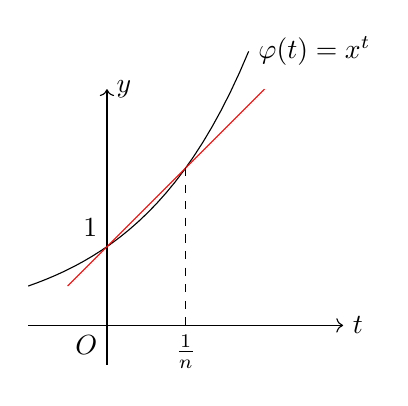
\begin{tikzpicture}
            \draw[->] (-1,0)--(3,0) node [right] {$t$};
            \draw[->] (0,-0.5)--(0,3) node [right] {$y$};
            \node at (0,0) [below left] {$O$};
            \node at (0,1) [above left] {$1$};
            \draw[domain=-1:1.8] plot(\x,{2^\x}) node [right] {$\varphi(t)=x^t$};
            \draw[-,red] (-0.5,0.5)--(2,3);
            \draw[-,dashed] (1,2)--(1,0) node [below] {$\frac{1}{n}$};
        \end{tikzpicture}
    \end{center}

    从而 $f_n(x)$ 单调不降且 $f_n(x)\to -\varphi'(0)=-\ln x=\ln\frac{1}{x}$.

    由 Dini 定理知在任何紧区间 $[a,b]\subset(0,\infty)$ 上有 $f_n\rightrightarrows\ln\frac{1}{x}$.

    但另一方面,若取定义域为 $(0,+\infty)$,则
$$
\Delta_n=\sup_{x\in(0,\infty)}\abs{f(x)-f_n(x)}=+\infty
$$

    从而 $\Delta_n\not\to 0$. 故 $f_n\not\rightrightarrows\ln\frac{1}{x}$.
\end{proof}

\mysubsection{极限与积分运算}

\begin{theorem}\label{ucint}
    设 $f_t:[a,b]\to\RR,t\in T$ 是一族函数. 设 $\mathcal{B}_T$ 是 $T$ 的一个基. 若

    \begin{enumerate}
        \item $f_t\xrightrightarrows[\mathcal{B}_T]{}f$
        
        \item $\forall t\in T,f_t\in\mathcal{R}[a,b]$
    \end{enumerate}

    则 $f\in\mathcal{R}[a,b]$ 且
$$
\int_a^bf(x)\dd x=\lim_{\mathcal{B}_T}\int_a^bf_t(x)\dd x
$$
\end{theorem}
\begin{proof}
    我们希望使用第 2 节的抽象定理 \ref{sl}. 为此,我们必须找到一个合适的框架:回忆积分是一种特殊的极限,其是关于一个特殊的空间的一个特殊的基取极限.

    定义 $X=\set{(P,\xi)|(P,\xi)\text{ 为 }[a,b]\text{ 带标志点的分划}}$.

    对任意 $\delta>0$ 令 $B_\delta=\set{(P,\xi)\in X|\lambda(P)<\delta}$.
    
    则 $\mathcal{B}_X=\set{B_\delta|\delta>0}$ 构成 $X$ 的一个基.

    考虑一族函数 $F_t:X\to\RR$ 定义为
$$
F_t(P,\xi)\triangleq\sigma(f_t,P,\xi)=\sum_{j=1}^nf_t(\xi_j)\Delta_j
$$

    由 $f_t\xrightrightarrows[\mathcal{B}_T]{}f$ 知 $F_t\xrightrightarrows[\mathcal{B}_T]{}F$. 其中 $F(P,\xi)\triangleq\sigma(f,P,\xi)$.

    由 $f_t\in\mathcal{R}[a,b]$ 知
$$
\lim_{\mathcal{B}_X}F_t(P,\xi)=\int_a^bf_t(x)\dd x=A_t
$$

    存在. 从而抽象定理的条件满足. 由该定理可得 $\lim\limits_{\mathcal{B}_T}A_t$ 与 $\lim\limits_{\mathcal{B}_X}F(P,\xi)$ 均存在且
$$
\lim_{\mathcal{B}_T}\int_a^bf_t(x)\dd x=\lim_{\mathcal{B}_T}A_t=\lim_{\mathcal{B}_X}F(P,\xi)=\int_a^bf(x)\dd x
$$
\end{proof}

\begin{inference}
    设 $f_n:[a,b]\to\RR$ 满足 $f_n\in\mathcal{R}[a,b]$.

    且 $\sum\limits_{n=1}^\infty f_n(x)$ 在 $[a,b]$ 上一致收敛,则 $\sum\limits_{n=1}^\infty f_n\in\mathcal{R}[a,b]$ 且
$$
\int_a^b\sum\limits_{n=1}^\infty f_n(x)\dd x=\sum_{n=1}^\infty\int_a^b f_n(x)\dd x
$$
\end{inference}

\begin{example}
    在第一卷我们定义过函数
$$
\mathrm{Si}(x)\triangleq\int_0^x\frac{\sin t}{t}\dd t
$$

    现在利用刚证的性质我们可以给出 $\mathrm{Si}(x)$ 的一个幂级数公式. 事实上
$$
\frac{\sin x}{x}=\sum_{n=0}^\infty\frac{(-1)^nx^{2n}}{(2n+1)!}
$$

    由其收敛半径为 $+\infty$ 知该幂级数在任何有界区间上均一致收敛. 从而由推论可知
$$
\begin{aligned}
    \mathrm{Si}(x)&=\int_0^x\frac{\sin t}{t}\dd t=\sum_{n=0}^\infty\frac{(-1)^n}{(2n+1)!}\int_0^xt^{2n}\dd t\\
    &=\sum_{n=0}^\infty\frac{(-1)^nx^{2n+1}}{(2n+1)!(2n+1)}
\end{aligned}
$$

    其收敛半径仍为 $+\infty$.

    特别的,在任何有界区间上,我们可以用多项式来一致逼近 $\mathrm{Si}(x)$.
\end{example}

\mysubsection{极限与微分运算}

接下来,我们讨论可微函数列在取完极限之后保持可微性的条件.

\begin{theorem}\label{limd}
    设 $X\subset\RR^n$ 为有界凸集. 设 $f_t:X\to\RR,t\in T$ 是一族函数. 设 $\mathcal{B}$ 是 $T$ 的一个基.

    若以下三个条件成立

    \begin{enumerate}
        \item $\forall t\in T,f_t$ 均在 $X$ 上可导.
        
        \item $f_t'\xrightrightarrows[\mathcal{B}]{}\varphi:X\to\RR$.
        
        \item $\exists x_0\in X,\lim\limits_{\mathcal{B}}f_t(x_0)$ 存在.
    \end{enumerate}

    则 $f_t\xrightrightarrows[\mathcal{B}]{}{f}$ 且 $f$ 在 $X$ 上可导,$f'=\varphi$.
\end{theorem}
\begin{proof}
    先证 $f_t\xrightrightarrows[\mathcal{B}]{}f$. 为此我们验证 Cauchy 准则:

    任取 $x\in X,t_1,t_2\in T$. 由有限增量定理
$$
\abs{f_{t_1}(x)-f_{t_2}(x)-(f_{t_1}(x_0)-f_{t_2}(x_0))}\le\sup_{\xi\in[x_0,x]}\norm{f_{t_1}'(\xi)-f_{t_2}'(\xi)}\abs{x-x_0}
$$

    由 $f_t'\xrightrightarrows[\mathcal{B}]{}\varphi$ 以及 $\lim\limits_{\mathcal{B}}f_t(x_0)$ 存在知
$$
\forall\eps>0,\exists B\in\mathcal{B},\forall t_1,t_2\in B,\forall x\in K,\norm{f_{t_1}'(x)-f_{t_2}'(x)}<\eps,\abs{f_{t_1}(x_0)-f_{t_2}(x_0)}<\eps
$$

    从而对 $\forall x\in X$ 有
$$
\abs{f_{t_1}(x)-f_{t_2}(x)}<\eps+\eps d(X)
$$

    由 Cauchy 准则知 $\set{f_t}$ 在 $\mathcal{B}$ 下一致收敛.

    记 $f_t\xrightrightarrows[\mathcal{B}]{}f$. 下证 $f$ 在 $X$ 上可微且 $f'=\varphi$.

    为此我们需证:若 $x\in X,x+h\in X$ 有
$$
F(h)\triangleq\frac{\abs{f(x+h)-f(x)-\varphi(x)h}}{\abs{h}}\to 0\quad(h\to 0)
$$

    我们希望使用定理 \ref{sl} 来证明该结论. 为此考虑
$$
F_t(h)\triangleq\frac{\abs{f_t(x+h)-f_t(x)-f_t'(x)h}}{\abs{h}}
$$

    一方面,对于固定的 $t\in T$ 由 $f_t$ 在 $x$ 处可导知
$$
\lim_{h\to 0}F_t(h)=0
$$

    另一方面,我们来验证 $F_t(h)\xrightrightarrows[\mathcal{B}]{}F(h)$.

    首先显然有 $F_t(h)\xrightarrow[\mathcal{B}]{}F(h)$.

    从而只需对 $\set{F_t(h):t\in T}$ 验证 Cauchy 准则.

    任取 $t_1,t_2\in T$ 由有限增量定理有
$$
\begin{aligned}
    &\abs{(f_{t_1}(x+h)-f_{t_1}(x)-f_{t_1}'(x)h)-(f_{t_2}(x+h)-f_{t_2}(x)-f_{t_2}'(x)h)}\\
    \le&\sup_{\xi\in[x,x+h]}\norm{(f_{t_1}'(\xi)-f_{t_2}'(\xi))-(f_{t_1}'(x)-f_{t_2}'(x))}\abs{h}
\end{aligned}
$$

    由 $f_t'\xrightrightarrows[\mathcal{B}]{}\varphi$ 知
$$
\forall\eps>0,\exists B\in\mathcal{B},\forall t_1,t_2\in B,\forall x\in X,\norm{f_{t_1}'(x)-f_{t_2}'(x)}<\eps
$$

    从而对 $\forall h\ne 0$ 有
$$
\abs{F_{t_1}(h)-F_{t_2}(h)}<\frac{(\eps+\eps)\abs{h}}{\abs{h}}=2\eps
$$

    即 $\set{F_t}$ 在 $\mathcal{B}$ 下一致收敛. 从而 $F_t\xrightrightarrows[\mathcal{B}]{}F$.

    现在由定理 \ref{sl} 知 $\lim\limits_{h\to 0}F(h)$ 与 $\lim\limits_{\mathcal{B}}\lim\limits_{h\to 0}F_t(h)$ 均存在且二者相等.

    从而 $\lim\limits_{h\to 0}F(h)=0$. 即 $f$ 在 $x$ 处可导且 $f'(x)=\varphi(x)$.
\end{proof}

\begin{inference}
    设 $X\subset\RR^n$ 为有界凸集. 设 $f_n:X\to\RR$ 在 $X$ 上可微.

    设 $\sum\limits_{n=1}^\infty f_n'(x)$ 在 $X$ 上一致收敛,且 $\exists x_0\in X,\sum\limits_{n=1}^\infty f_n(x_0)$ 收敛.

    则 $\sum\limits_{n=1}^\infty f_n(x)$ 在 $X$ 上一致收敛,极限函数可微且满足
$$
\left(\sum\limits_{n=1}^\infty f_n(x)\right)'=\sum\limits_{n=1}^\infty f_n'(x)
$$
\end{inference}

作为应用,我们来讨论幂级数的逐项求导与逐项积分.

\begin{property}
    设幂级数 $\sum\limits_{n=0}^\infty a_n(z-z_0)^n$ 的收敛半径 $R>0$. 则

    \begin{enumerate}
        \item 该幂级数在 $z_0+D_R$ 上 $C^{(1)}$ 光滑,且极限函数 $S$ 可微,有
$$
S'(x)=\sum_{n=1}^\infty na_n(z-z_0)^{n-1}
$$

        \item 对任意光滑路径 $\gamma:[0,1]\to z_0+D_r$ 满足 $\gamma(0)=z_0,\gamma(1)=z$ 有
$$
\int_\gamma S(z)\dd z=\sum_{n=0}^\infty\frac{a_n}{n+1}(z-z_0)^{n+1}
$$
    \end{enumerate}
\end{property}

\img{0.4}{16.3.1.png}

\begin{proof}
    \begin{enumerate}
        \item 在第一学期我们就证明过这个结论. 但在这里,我们用新的知识来重新证明一遍.
        
        令 $f_n(z)=a_n(z-z_0)^n$. 则 $f_n$ 可微且 $f_n'(z)=na_n(z-z_0)^{n-1}$.

        由 $\overline{\lim\limits_{n\to\infty}}\sqrt[n]{n\abs{a_n}}=\dfrac{1}{R}$ 知 $\sum\limits_{n=0}^\infty f_n'(z)$ 在 $z_0+D_r$ 上一致收敛,$\forall 0<r<R$.

        且 $\sum\limits_{n=0}^\infty f_n(z_0)$ 显然收敛. 从而由上一推论可知:$\sum\limits_{n=0}^\infty f_n(z)$ 也一致收敛且可微,且有
$$
\left(\sum_{n=0}^\infty a_n(z-z_0)^n\right)'=\sum_{n=1}^\infty na_n(z-z_0)^{n-1}
$$

        \item 取 $0<r<R$ 使得 $\gamma([0,1])\subset z_0+\overline{D_r}$.
        
        则由 $\sum\limits_{n=0}^\infty a_n(z-z_0)^n$ 在 $z_0+\overline{D_r}$ 上一致收敛知
$$
\sum\limits_{n=0}^\infty a_n(\gamma(t)-z_0)^n\gamma'(t)
$$

        在 $[0,1]$ 上一致收敛. 从而由积分与求和可交换次序知
$$
\begin{aligned}
    &\int_\gamma\sum\limits_{n=0}^\infty a_n(z-z_0)^n\dd z=\int_0^1\sum\limits_{n=0}^\infty a_n(\gamma(t)-z_0)^n\gamma'(t)\dd t\\
    =&\sum\limits_{n=0}^\infty a_n\int_0^1(\gamma(t)-z_0)^n\gamma'(t)\dd t=\sum_{n=0}^\infty a_n\int_0^1\frac{\dd(\gamma(t)-z_0)^{n+1}}{n+1}\\
    =&\sum\limits_{n=0}^\infty \frac{a_n}{n+1}(z-z_0)^{n+1}
\end{aligned}
$$
    \end{enumerate}
\end{proof}

\begin{example}
    Bessel 函数 $J_n(x)$ 为如下微分方程的解:
$$
x^2y''+xy'+(x^2-n^2)y=0
$$

    我们可以使用幂级数法来求解该方程.

    例如在 $n=0$ 时
$$
J_0(x)=1+\sum\limits_{k=1}^\infty(-1)^k\frac{x^{2k}}{(k!)^22^{2k}}
$$
\end{example}


\mysection{连续函数空间的紧子集与稠密子集}

本节,我们证明两个十分重要的定理. 它们分别刻画了紧空间上的连续函数空间的紧子集与稠密子集.

\mysubsection{Arzelà-Ascoli 定理}

\begin{definition}
    设 $X$ 为集合,$(Y,\rho)$ 为度量空间. 设 $\mathscr{F}=\set{f:X\to Y}$ 为一族函数.

    称 $\mathscr{F}$ 一致有界,若所有 $f\in\mathscr{F}$ 的值域之并在 $Y$ 中有界. 即
$$
V\triangleq\set{f(x)|x\in X,f\in\mathscr{F}}
$$

    在 $Y$ 中有界.

    称 $\mathscr{F}$ 完全有界,若 $V$ 是 $Y$ 中的完全有界集.
\end{definition}

\begin{hint}
    若 $Y=\RR^n$ 或 $\mathbb{C}^n$,则 $A\subset Y$ 有界 $\iff A$ 完全有界.

    从而在此时函数族 $\mathscr{F}$ 一致有界与完全有界等价.

    但若 $Y$ 为无穷维赋范线性空间,则完全有界的概念严格强于有界. 例如 $Y=C[a,b]$.
\end{hint}

\begin{definition}
    设 $(X,d),(Y,\rho)$ 均为度量空间,$\mathscr{F}=\set{f:X\to Y}$ 为一族函数.

    称 $\mathscr{F}$ 等度连续,若
$$
\forall\eps>0,\exists\delta>0,\forall x_1,x_2\in X,d(x_1,x_2)<\delta\implies\forall f\in\mathscr{F},\rho(f(x_1),f(x_2))<\eps
$$
\end{definition}

\begin{example}
    $\mathscr{F}=\set{x^n|n\ge 1},X=[0,1]$.

    则 $\mathscr{F}$ 一致有界,但不等度连续.
\end{example}

\begin{example}
    $\mathscr{F}=\set{\sin nx|n\in\mathbb{N}}$ 在任何区间 $[a,b]$ 上均不等度连续.
\end{example}

\begin{example}
    若 $\mathscr{F}$ 是一族从 $\RR$ 到 $\RR$ 的映射,且
$$
\exists L>0,\forall f\in\mathscr{F},\forall x,y\in\RR,\abs{f(x)-f(y)}\le L\abs{x-y}
$$

    则 $\mathscr{F}$ 等度连续.
\end{example}

如上的概念与一致收敛性有密切的连续:

\begin{lemma}
    设 $K$ 为紧度量空间,$Y$ 为完备度量空间.

    设 $f_n\in C(K;Y)$. 若 $\set{f_n}$ 在 $K$ 上一致收敛,则 $\set{f_n}$ 在 $K$ 上完全有界且等度连续.
\end{lemma}
\begin{proof}
    设 $f_n\rightrightarrows f:K\to Y$. 则 $f$ 也连续.

    \begin{itemize}
        \item 完全有界:
        
        由 $f_n,f$ 连续且 $K$ 紧知 $f_n(K),f(K)$ 均为 $Y$ 中的紧集. 从而完全有界. 由 $f(K)$ 完全有界知
$$
\forall\eps>0,\exists x_1,\cdots,x_k\in K,f(K)\subset\bigcup_{j=1}^kB\left(f(x_j),\frac{\eps}{2}\right)
$$

        由 $f_n\rightrightarrows f$ 知
$$
\begin{aligned}
    \exists N\in\mathbb{N},\forall n\ge N,&\forall x\in K,\abs{f_n(x)-f(x)}<\frac{\eps}{2}\\
    \implies&f_n(K)\subset\bigcup_{j=1}^kB(f(x_j),\eps)
\end{aligned}
$$

        故 $\bigcup\limits_{n\ge N}f_n(K)$ 完全有界.

        由 $f_1(K)\cup\cdots\cup f_N(K)$ 是有限个完全有界集之并,知其完全有界. 故
$$
V\triangleq\bigcup_{n=1}^\infty f_n(K)=\bigcup_{n=1}^Nf_n(K)\cup\bigcup_{n\ge N}f_n(K)
$$

        完全有界. 即 $\set{f_n}$ 完全有界.
        
        \item 等度连续:
        
        任取 $\eps>0$. 由 $f_n\rightrightarrows f$ 知
$$
\exists N\in\mathbb{N},\forall n\ge N,\forall x\in K,\abs{f_n(x)-f(x)}<\frac{\eps}{3}
$$

        由 $f_1,\cdots,f_N,f$ 在紧集 $K$ 上连续知它们一致连续. 从而
$$
\begin{aligned}
    \exists\delta>0,\forall x,x'\in K,d(x,x')<\delta\implies&\rho(f_j(x),f_j(x'))<\frac{\eps}{3},1\le j\le N\\
    &\rho(f(x),f(x'))<\frac{\eps}{3}
\end{aligned}
$$

        则对 $n\ge N$ 有
$$
\begin{aligned}
    \forall x,x'\in K,d(x,x')<\delta\implies&\rho(f_n(x),f_n(x'))\\
    \le&\rho(f_n(x),f(x))+\rho(f(x),f(x'))+\rho(f(x'),f_n(x'))\\
    <&\frac{\eps}{3}+\frac{\eps}{3}+\frac{\eps}{3}=\eps
\end{aligned}
$$

        即 $\set{f_n}$ 等度连续.
    \end{itemize}
\end{proof}

现在我们可以陈述 Arzelà-Ascoli 定理.

\begin{theorem}[Arzelà-Ascoli]
    设 $\mathscr{F}$ 是一族从紧度量空间 $K$ 到完备度量空间 $Y$ 的函数. 则

    $\forall\set{f_n}\subset\mathscr{F}$,存在子列 $n_k$ 使得 $\set{f_{n_k}}$ 一致收敛 $\iff\mathscr{F}$ 完全有界且等度连续.
\end{theorem}
\begin{proof}
    $\implies$:反证,设 $\mathscr{F}$ 不完全有界,即 $V=\set{f(x)|x\in K,f\in\mathscr{F}}$ 不完全有界.
    
    即存在 $\eps_0>0$ 使得 $V$ 不存在有限 $\eps_0$-网.

    则可以构造 $f_n\in\mathscr{F},x_n\in K$ 满足
$$
\rho(f_n(x_n),f_m(x_m))\ge\eps_0,\forall n\ne m
$$

    这说明 $\set{f_n}\subset\mathscr{F}$ 不完全有界,且 $\set{f_n}$ 的任何子列也不完全有界. 从而由引理知其不可能一致收敛.

    反证,设 $\mathscr{F}$ 不等度连续.

    则存在 $\eps_0>0$ 以及 $f_n\in\mathscr{F},x_n,x_n'\in K$ 满足
$$
\begin{cases}
    d(x_n,x_n')<\dfrac{1}{n}\\
    \rho(f_n(x_n),f_n(x_n'))\ge\eps_0
\end{cases},\forall n\in\mathbb{N}
$$

    则 $\set{f_n}$ 的任何子列都不等度连续. 从而不可能一致收敛.

    $\impliedby$:下设 $\mathscr{F}$ 完全有界且等度连续.

    设 $\set{f_n}\subset\mathscr{F}$. 由 $K$ 紧知:存在可数集 $D\subset K$ 使得 $\overline{D}=K$.

    可以这样构造:$\forall n\in\mathbb{N}$ 存在 $K$ 的有限 $\dfrac{1}{n}$-网 $D_n$. 令 $D=\bigcup\limits_{n\in\mathbb{N}}D_n$ 即可.

    现在对 $\set{f_n}$ 利用 Cantor 对角线法,可以选出子列 $\set{f_{n_k}}$ 使得 $\forall x\in D$ 有 $f_{n_k}(x)\to f_\infty(x),k\to\infty$.

    这里能选出子列的原因是 $\forall x\in D,\set{f_n(x)}$ 完全有界且 $Y$ 完备.

    下证:$\set{f_{n_k}}$ 一致收敛.

    任取 $\eps>0$. 由 $\mathscr{F}$ 等度连续知
$$
\exists\delta>0,\forall f\in\mathscr{F},\forall x,x'\in K,d(x,x')<\delta\implies\rho(f(x),f(x'))<\frac{\eps}{4}
$$

    由 $D\subset K$ 知 $D$ 完全有界. 从而其存在有限 $\dfrac{\delta}{2}$-网,记为 $\set{x_1,\cdots,x_m}\subset D$.

    由 $f_{n_k}(x_i)\to f_\infty(x_i),i=1,\cdots,m$ 知
$$
\exists K\in\mathbb{N},\forall k\ge K,\forall 1\le i\le m,\rho(f_{n_k}(x_i),f_\infty(x_i))<\frac{\eps}{4}
$$

    现任取 $k,l\ge K$. 则对 $\forall x\in K$ 可以选出 $x_i$ 使得 $d(x,x_i)<\delta$. 从而
$$
\begin{aligned}
    \rho(f_{n_k}(x),f_{n_l}(x))\le&\rho(f_{n_k}(x),f_{n_k}(x_i))+\rho(f_{n_k}(x_i),f_\infty(x_i))\\
    &+\rho(f_\infty(x_i),f_{n_l}(x_i))+\rho(f_{n_l}(x_i),f_{n_l}(x))\\
    <&\frac{\eps}{4}+\frac{\eps}{4}+\frac{\eps}{4}+\frac{\eps}{4}=\eps
\end{aligned}
$$

    即 $\set{f_{n_k}}$ 满足 Cauchy 准则,从而一致收敛.
\end{proof}

\mysubsection{度量空间 $C(K;Y)$}

我们先来回顾一些度量空间相关的结论.

\begin{property}
    设 $X$ 为度量空间. 则 $A\subset X$ 紧 $\iff A$ 列紧 $\iff A$ 完全有界且完备.
\end{property}

\begin{definition}
    设 $X$ 为度量空间. 称 $A\subset X$ 为预紧集,若 $\overline{A}\subset X$ 为紧集. 
\end{definition}

\begin{property}
    若 $X$ 为完备度量空间,则 $A\subset X$ 为预紧集 $\iff A$ 完全有界.
\end{property}
\begin{proof}
    $\implies$:$A$ 预紧 $\implies\overline{A}$ 紧 $\implies\overline{A}$ 完全有界 $\implies A$ 完全有界.

    $\impliedby$:$A$ 完全有界 $\implies\overline{A}$ 闭且完全有界 $\implies A$ 紧 $\implies A$ 预紧.
\end{proof}

以下我们来解释 A-A 定理的含义. 在第九章中我们已经知道:若 $K$ 为紧度量空间,$Y$ 为完备度量空间,则 $C(K;Y)$ 在如下的范数下成为一个 Banach 空间
$$
\norm{f}_\infty\triangleq=\sup_{x\in K}\abs{f(x)}=\max_{x\in K}\abs{f(x)}
$$

若 $f_n,f\in C(K;Y)$,则
$$
f_n\rightrightarrows f\iff\norm{f_n-f}_\infty\to 0
$$

即空间 $C(K;Y)$ 中的“点列” $\set{f_n}$ 收敛到“点” $f$.

在这个语言下,A-A 定理可以表述为:

\begin{property}
    设 $\mathscr{F}\subset C(K;Y)$. 则:
    
    $\forall\set{f_n}\subset\mathscr{F}$ 均存在收敛子列 $\set{f_{n_k}}\iff\mathscr{F}$ 完全有界且等度连续.
\end{property}

其中前者的含义即为 $\mathscr{F}$ 预列紧(即 $\overline{\mathscr{F}}$ 列紧).

从而 A-A 定理给出的是 $C(K;Y)$ 中预列紧集的一个刻画. 从而我们进一步得到

\begin{property}
    设 $\mathscr{F}\subset C(K;Y)$. 则 $\mathscr{F}$ 列紧 $\iff\mathscr{F}$ 完全有界、等度连续且 $\mathscr{F}$ 闭.
\end{property}

接下来,我们讨论如何判定 $C(K;Y)$ 的一个子集是否稠密. 这在实际应用中非常重要.

作为一个热身,我们首先来证明经典的 Weierstrass 定理.

用 $\mathscr{P}$ 表示所有一元实系数多项式的全体.

\begin{theorem}[Weierstrass]
    $\mathscr{P}$ 在 $C([a,b];\RR)$ 中稠密. 等价的,$\overline{\mathscr{P}}=C([a,b])$.

    或 $\forall f\in C[a,b],\exists\set{P_n}\subset\mathscr{P},\norm{P_n-f}_\infty\to 0$.
\end{theorem}

\begin{hint}
    我们曾经使用 Bernstein 多项式证明了上述定理. 这里我们采用完全不同的方法来证明.

    而这个证明的想法,可以用来证明下一节更为一般的 Stone 定理.
\end{hint}

我们先来做一些观察:

\begin{lemma}
    记所有分段线性连续函数全体为 $\mathscr{L}$,则
$$
\overline{\mathscr{L}}=C[a,b]
$$
\end{lemma}
\begin{proof}
    由一致连续性可得.
\end{proof}

\begin{center}
    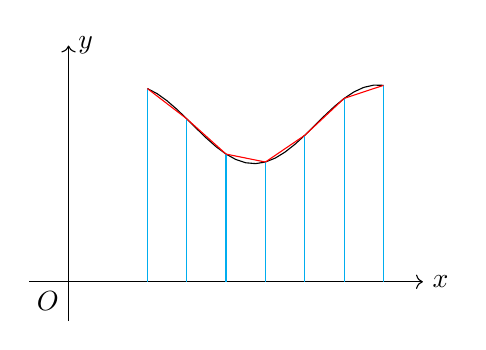
\begin{tikzpicture}
        \draw[->] (-0.5,0)--(4.5,0) node [right] {$x$};
        \draw[->] (0,-0.5)--(0,3) node [right] {$y$};
        \node at (0,0) [below left] {$O$};

        \draw[domain=1:4] plot (\x,{2+0.5*sin(2*\x r)});

        \foreach \i in {0,...,6} {
            \draw[-,cyan] (1+\i/2,0)--(1+\i/2,{2+0.5*sin((2+\i)r)});
        }
        \foreach \i in {0,...,5} {
            \draw[-,red] (1+\i/2,{2+0.5*sin((2+\i)r)})--(1.5+\i/2,{2+0.5*sin((3+\i)r)});
        }
    \end{tikzpicture}
\end{center}

记 $\mathscr{A}=\overline{\mathscr{P}}$.

\begin{lemma}
    $\mathscr{A}$ 是一个代数. 即若 $f,g\in\mathscr{A}$,则
$$
\lambda f+\mu g\in\mathscr{A},\forall\lambda,\mu\in\RR,\qquad f\cdot g\in\mathscr{A}
$$
\end{lemma}
\begin{proof}
    设 $P,Q\in\mathscr{P}$ 满足 $\norm{P-f}_\infty<\eps,\norm{Q-g}<\eps$. 则
$$
\begin{aligned}
    \norm{(\lambda P+\mu Q)-(\lambda f+\mu g)}&\le(\abs{\lambda}+\abs{\mu})\eps\\
    \norm{PQ-fg}\le\norm{P(Q-g)}+&\norm{g(P-f)}\le(\norm{P}+\norm{g})\eps\le(\norm{f}+\norm{g}+\eps)\eps
\end{aligned}
$$
\end{proof}

任给 $a\le\xi_1<\xi_2\le b$. 定义
$$
g_{\xi_1,\xi_2}(x)\triangleq\frac{x-\xi_1}{\xi_2-\xi_1}
$$

令
$$
F_{\xi_1,\xi_2}(x)\triangleq 0\wedge g_{\xi_1,\xi_2}\qquad G_{\xi_1,\xi_2}\triangleq 1\vee F_{\xi_1,\xi_2}
$$

其中 $f\wedge g\triangleq\max\set{f,g},f\vee g\triangleq\min\set{f,g}$.

\begin{center}
    \begin{tikzpicture}[scale=1.5]
        \draw[->] (-0.5,0)--(5,0) node [right] {$y$};
        \draw[->] (0,-0.5)--(0,3) node [right] {$x$};
        \node at (0,0) [below left] {$O$};
        \draw[-] (1,0.05)--(1,-0.05) node [below] {$a$};
        \draw[-] (2,0.05)--(2,-0.05) node [below] {$\xi_1$};
        \draw[-] (3,0.05)--(3,-0.05) node [below] {$\xi_2$};
        \draw[-] (4,0.05)--(4,-0.05) node [below] {$b$};
        \draw[-,dashed] (3,2)--(0,2) node [left] {$1$};
        \draw[-,dashed] (3,0)--(3,2);
        \draw[-,red] (1.7,-0.6)--(3.4,2.8) node [right] {$g_{\xi_1,\xi_2}$};
        \draw[-,blue] (-0.5,0.05)--(1.95,0.05);
        \draw[-,blue] (1.95,0.05)--(3.3,2.75) node [left] {$F_{\xi_1,\xi_2}$};
        \draw[-] (-0.5,0.1)--(1.9,0.1);
        \draw[-] (1.9,0.1)--(2.85,2);
        \draw[-] (2.85,2)--(5,2) node [right] {$G_{\xi_1,\xi_2}$};
    \end{tikzpicture}
\end{center}

\begin{lemma}
    令 $\mathscr{G}=\set{G_{\xi_1,\xi_2}|a\le\xi_1<\xi_1\le b}\cup\set{1}$.

    则 $\mathrm{span}\;\mathscr{G}=\mathscr{L}$. 即
$$
\forall f\in\mathscr{L},\exists\set{g_1,\cdots,g_m}\subset\mathscr{G},\lambda_1,\cdots,\lambda_m\in\RR,f=\sum_{j=1}^m\lambda_jg_j
$$
\end{lemma}
\begin{proof}
    直接验证.
\end{proof}

由以上引理,为了证明 Weierstrass 定理,我们仅需证明 $\mathscr{G}\subset\mathscr{A}$.

这是因为:若 $\mathscr{G}\subset\mathscr{A}$,则由 $\mathscr{A}$ 为代数知 $\mathscr{L}\subset\mathscr{A}$. 从而 $C[a,b]=\overline{\mathscr{L}}\subset\mathscr{A}$.

从而问题归结为:是否对 $\forall a\le\xi_1<\xi_2\le b$ 有 $G_{\xi_1,\xi_2}\in\mathscr{A}$.

注意到
$$
f\vee g=\frac{f+g-\abs{f-g}}{2}\qquad f\wedge g=\frac{f+g+\abs{f-g}}{2}
$$

从而由 $G_{\xi_1,\xi_2}$ 的定义方式知,如果能够证明如下的关键引理,则结论成立.

\begin{lemma}
    若 $f\in\mathscr{A}$,则 $\abs{f}\in\mathscr{A}$.
\end{lemma}
\begin{proof}
    固定 $f\in\mathscr{A}$. 设 $\norm{f}_\infty\le M$.

    断言存在 $\set{Q_n}\subset\mathscr{P}$ 使得在 $[-M,M]$ 上
$$
Q_n\rightrightarrows\abs{\;\cdot\;}
$$

    \textbf{证明:}当 $M=1$ 时,我们已经证明存在 $\set{\widetilde{Q}_n}\subset\mathscr{P}$ 使得在 $[-1,1]$ 上
$$
\widetilde{Q}_n\rightrightarrows\abs{\;\cdot\;}
$$

    令 $Q_n(y)\triangleq M\widetilde{Q}_n\left(\dfrac{y}{M}\right)$. 则 $Q_n$ 满足条件.

    \qed

    由 $\norm{f}_\infty\le M$ 以及断言知
$$
\norm{\abs{f}-Q_n(f)}_\infty\to 0
$$

    由 $f\in\mathscr{A}$ 以及 $\mathscr{A}$ 为代数知 $Q_n(f)\in\mathscr{A},\forall n\in\mathbb{N}$.

    从而上式说明 $Q_n(f)\rightrightarrows\abs{f}$. 由 $\mathscr{A}$ 闭知 $\abs{f}\in\mathscr{A}$.
\end{proof}

现任给 $a\le\xi_1<\xi_2\le b$. 则有
$$
0,g_{\xi_1,\xi_2}\in\mathscr{A}\implies F_{\xi_1,\xi_2}\in\mathscr{A}\implies G_{\xi_1,\xi_2}\in\mathscr{A}
$$

从而 Weierstrass 定理即证.

\mysubsection{Stone 定理}

我们最后在证明一个大大推广的 Weierstrass 定理:Stone 定理. 为此,我们先介绍几个概念.

\begin{definition}
    设 $\mathscr{A}$ 是一族从 $X$ 到 $\RR(\mathbb{C})$ 的函数.

    称 $\mathscr{A}$ 是一个实(复)函数代数,若 $\forall f,g\in\mathscr{A}$ 有
$$
\lambda f+\mu g\in\mathscr{A},\forall\lambda,\mu\in\RR(\mathbb{C}),\qquad f\cdot g\in\mathscr{A}
$$
\end{definition}

\begin{example}
    所有多项式的全体 $\mathscr{P}$ 为函数代数.
\end{example}

\begin{example}
    $\mathscr{A}_1\triangleq\mathrm{span}\set{e^{nx}|n\ge 0}$ 为函数代数.
\end{example}

\begin{example}
    $\mathscr{A}_1\triangleq\mathrm{span}\set{e^{inx}|n\in\mathbb{Z}}$ 为函数代数.
\end{example}

\begin{definition}
    设 $\mathscr{F}$ 是一族从 $X$ 到 $Y$ 的映射.

    称 $\mathscr{F}$ 在 $X$ 上分点,若
$$
\forall x_1,x_2\in X,x_1\ne x_2\implies\exists f\in\mathscr{F},f(x_1)\ne f(x_2)
$$
\end{definition}

\begin{example}
    $\mathscr{P}$ 在 $\RR$ 上分点,$\mathscr{A}_1$ 在 $\RR$ 上分点.

    若 $b-a<2\pi$,则 $\mathscr{A}_2$ 在 $[a,b]$ 上分点,反之不分点.
\end{example}

\begin{definition}
    设 $\mathscr{F}$ 是一族从 $X$ 到 $\RR(\mathbb{C})$ 的函数.

    称 $\mathscr{F}$ 在 $X$ 上非退化,若 $\forall x\in X,\exists f\in\mathscr{F},f(x)\ne 0$.
\end{definition}

\begin{example}
    $\set{1,x,x^2,\cdots}$ 在 $[0,1]$ 上非退化,但 $\set{x,x^2,\cdots}$ 在 $[0,1]$ 上退化.
\end{example}

\begin{lemma}
    设 $\mathscr{A}$ 是 $X$ 上的实(复)函数代数,其在 $X$ 上分点且非退化.

    则 $\forall x_1,x_2\in X,x_1\ne x_2,\forall c_1,c_2\in\RR(\mathbb{C})$ 均存在 $s\in\mathscr{A}$ 使得
$$
s(x_1)=c_1,s(x_2)=c_2
$$
\end{lemma}
\begin{proof}
    由 $\mathscr{A}$ 为代数,我们仅需考虑 $c_1=1,c_2=0$ 以及 $c_1=0,c_2=1$ 的情形.

    由对称性,我们仅需考虑 $c_1=1,c_2=0$.

    断言:存在 $\varphi\in\mathscr{A}$ 使得 $\varphi(x_1)\ne\varphi(x_2)$ 且 $\varphi(x_1)\ne 0$.

    \textbf{证明:}由 $\mathscr{A}$ 分点知:存在 $g\in\mathscr{A}$ 使得 $g(x_1)\ne g(x_2)$.

    \begin{enumerate}
        \item 若 $g(x_1)\ne 0$. 则 $\varphi=g$ 满足条件.
        
        \item 若 $g(x_1)=0$. 则 $g(x_2)\ne 0$.
        
        由 $\mathscr{A}$ 在 $X$ 上非退化,存在 $h\in\mathscr{A}$ 使得 $h(x_1)=0$.

        令 $\varphi=g+\lambda h,\lambda\ne 0$. 则只要 $\lambda$ 足够小,$\varphi$ 就满足条件.
    \end{enumerate}

    \qed

    令 $S(x)=\dfrac{\varphi(x)^2-\varphi(x_2)\varphi(x)}{\varphi(x_1)^2-\varphi(x_1)\varphi(x_2)}\in\mathscr{A}$.

    则 $S(x_1)=1,S(x_2)=0$ 满足条件.
\end{proof}

现在我们可以证明最一般的稠密性定理.

\begin{theorem}[Stone]
    设 $K$ 为紧度量空间. 设 $\mathscr{A}\subset C(K;\RR)$ 为函数代数.

    若 $\mathscr{A}$ 在 $K$ 中分点且非退化,则 $\mathscr{A}$ 在 $C(K;\RR)$ 中稠密,即 $\overline{\mathscr{A}}=C(K;\RR)$.
\end{theorem}
\begin{proof}
    首先注意到 $\mathscr{A}$ 为代数 $\implies\overline{\mathscr{A}}$ 也为代数.

    任取 $f\in C(K;\RR)$. 由 $K$ 紧知 $\norm{f}_\infty\le M$. 从而利用上一定理的证明可得:
$$
f\in\overline{\mathscr{A}}\implies\abs{f}\in\overline{\mathscr{A}}
$$

    进而有:若 $f,g\in\overline{\mathscr{A}}$,则
$$
f\wedge g=\frac{f+g+\abs{f-g}}{2}\in\overline{\mathscr{A}}\qquad f\vee g=\frac{f+g-\abs{f-g}}{2}\in\overline{\mathscr{A}}
$$

    归纳的有
$$
f_1,\cdots,f_n\in\overline{\mathscr{A}}\implies f_1\wedge\cdots\wedge f_n,f_1\vee\cdots\vee f_n\in\overline{\mathscr{A}}
$$

    现固定 $f\in C(K),\eps>0$.

    断言 1:对 $\forall x\in K,\exists\varphi_x\in\overline{\mathscr{A}}$ 使得
$$
\varphi_x(x)=f(x)\qquad\varphi_x(y)\ge f(y)-\eps,\forall y\in K
$$

    \textbf{证明:}任取 $y\in K,y\ne x$. 由引理知,存在 $\eta_y\in\mathscr{A}$ 使得
$$
\eta_y(x)=f(x),\eta_y(y)=f(y)
$$

    由 $\eta_y,f$ 在 $y$ 处连续知:存在 $y$ 的邻域 $U_y$ 使得
$$
\forall z\in U_y,\eta_y(z)\ge f(z)-\eps
$$

    固定某点 $y_0\ne x$. 由 $\eta_{y_0},f$ 在 $x$ 处连续知:存在 $x$ 的邻域 $V_x$ 使得
$$
\forall z\in V_x,\eta_{y_0}(z)\ge f(z)-\eps
$$

    由 $K$ 紧以及 $\set{U_y|y\ne x}\cup\set{V_x}$ 为 $K$ 的开覆盖,存在有限子覆盖 $\set{U_{y_1},\cdots,U_{y_k},V_x}$.

    令 $\varphi_x\triangleq\eta_{y_1}\wedge\cdots\wedge\eta_{y_k}\wedge\eta_{y_0}\in\overline{\mathscr{A}}$.

    则 $\forall z\in K,\exists 1\le i\le k,z\in U_{y_i}$ 或 $z\in V_x$. 从而
$$
\begin{aligned}
    &\varphi_x(z)\ge\eta_{y_i}(z)\ge f(z)-\eps\\
    \text{或 }&\varphi_x(z)\ge\eta_{y_0}(z)\ge f(z)-\eps
\end{aligned}
$$

    \qed

    断言 2:存在 $\varphi\in\overline{\mathscr{A}}$ 使得
$$
\forall z\in K,f(z)+\eps\ge\varphi(z)\ge f(z)-\eps
$$

    \textbf{证明:}任取 $x\in K$,由断言 1 取 $\varphi_x\in\overline{\mathscr{A}}$.

    则由 $\varphi_x,x$ 在 $x$ 处连续知:存在 $x$ 的邻域 $V_x$ 使得
$$
\forall z\in V_x,\varphi_x(z)\le f(z)+\eps
$$

    由 $K$ 紧以及 $\set{V_x|x\in K}$ 为 $K$ 的开覆盖知存在有限开覆盖 $\set{V_{x_1},\cdots,V_{x_m}}$.

    令 $\varphi\triangleq\varphi_{x_1}\vee\varphi_{x_2}\vee\cdots\vee\varphi_{x_m}$.

    则一方面同断言 1 可得
$$
\forall z\in K,\varphi(z)\le f(z)+\eps
$$

    另一方面,由断言 1 有
$$
\begin{aligned}
    &\forall 1\le i\le m,\forall z\in K,\varphi_{x_i}(z)\ge f(z)-\eps\\
    \implies&\forall z\in K,\varphi(z)\ge f(z)-\eps
\end{aligned}
$$

    \qed

    断言 2 说明 $\norm{f-\varphi}_\infty<\eps$ 且 $\varphi\in\overline{\mathscr{A}}$.

    由 $\eps$ 的任意性以及 $\overline{\mathscr{A}}$ 闭知 $f\in\overline{\mathscr{A}}$.

    由 $f\in C[a,b]$ 的任意性知 $\overline{\mathscr{A}}=C[a,b]$.
\end{proof}

\mychapter{含参变量的积分}

本章我们研究含参变量积分的核心理论. 我们首先研究一元积分情形,最后再研究重积分的情形.

\mysection{依赖于一个参数的(正常)积分}

\mysubsection{基本框架}

如下形式的积分称为含参积分:
$$
F(t)=\int_{E_t}f(x,t)\dd x\qquad t\in T
$$

这里 $t$ 为参数,而 $E_t$ 是随 $t$ 变化的积分区域,$f(x,t)$ 是以 $t$ 为参数的一族函数.

\begin{itemize}
    \item 若对 $\forall t\in T$,积分 $\displaystyle\int_{E_t}f(x,t)\dd x$ 均为正常积分,则称 $F(t)$ 为含参变量的正常积分.
    
    \item 若 $\exists t\in T$ 使得积分 $\displaystyle\int_{E_t}f(x,t)\dd x$ 为广义积分,则称 $F(t)$ 为含参变量的广义积分.
\end{itemize}

本节,我们研究最简单的情形.

\mysubsection{含参积分的连续性}

\begin{property}
    设 $R\triangleq[a,b]\times[c,d]\subset\RR^2$ 为紧二维区间. 设 $f\in C(R)$,则
$$
F(y)\triangleq\int_a^bf(x,y)\dd x
$$

    在 $[c,d]$ 上连续.
\end{property}
\begin{proof}
    固定 $y_0\in[c,d]$. 下证 $F$ 在 $y_0$ 处连续.

    由 $f$ 在 $R$ 上一致连续知 $f_y\rightrightarrows f_{y_0},y\to y_0$.

    其中 $f_y(x)\triangleq f(x,y)$. 由 $f_y$ 连续知其 Riemann 可积.

    从而由定理 \ref{ucint} 知
$$
F(y)=\int_a^bf_y(x)\to\int_a^bf_{y_0}(x)\dd x=F(y_0)
$$
\end{proof}

\begin{hint}
    \begin{enumerate}
        \item 从证明过程来看,我们可以将 $[c,d]$ 换成任意一个紧集 $K\subset\RR$,结论依然成立.
        
        \item 有了这一观察,我们可以进一步将 $[c,d]$ 换成开集 $D\subset\RR^n$.
        
        若 $f\in C([a,b]\times D)$,则结论依然成立.

        \item 当然这里也可以由定义来直接证明,只需用到 $f$ 的一致连续性.
        
        作为一个应用,我们可以证明以前的一个性质.
    \end{enumerate}
\end{hint}

\begin{property}
    设 $U\subset\RR^n$ 为开集. 设 $f\in C^{(1)}(U;\RR),x_0\in U$.

    则存在 $x_0$ 的邻域 $U(x_0)$ 以及连续映射 $\varphi:U(x_0)\to\RR^n$ 使得
$$
f(x)=f(x_0)+\varphi(x)(x-x_0)\text{ 且 }\varphi(x_0)=f'(x_0)
$$
\end{property}
\begin{proof}
    取 $r>0$ 使得 $B(x_0,r)\subset U$.

    任取 $x\in B(x_0,r)$,对 $F(t)\triangleq f(x_0+t(x-x_0))$ 应用 N-L 公式得
$$
\begin{aligned}
    f(x)-f(x_0)&=F(1)-F(0)=\int_0^1F'(t)\dd t\\
    &=\int_0^1f'(x_0+t(x_0-x))(x-x_0)\dd t\\
    &=\int_0^1f'(x_0+t(x_0-x))\dd t\cdot(x-x_0)
\end{aligned}
$$

    令 $\varphi_i(x)\triangleq\displaystyle\int_0^1f_i'(x_0+t(x-x_0))\dd t,1\le i\le n$.

    由以上的注记知 $\varphi_i$ 在 $B(x_0,r)$ 上连续. 从而 $\varphi=(\varphi_1,\cdots,\varphi_n)$ 也连续.

    且 $f(x)=f(x_0)+\varphi(x)(x-x_0),\varphi(x_0)=f'(x_0)$ 满足条件.
\end{proof}

\mysubsection{含参积分关于参数的微分}

\begin{property}
    设 $X\subset\RR^d$ 为紧凸集. 设 $f\in C([a,b]\times X;\RR)$.

    设 $f(t,x)$ 关于 $x$ 分量的微分存在且连续. 即 $\dfrac{\partial f}{\partial x}\in C([a,b]\times X)$. 则
$$
F(x)\triangleq\int_a^bf(t,x)\dd x\in C^{(1)}(X)
$$

    且
$$
F'(x)=\int_a^b\pard{f}{x}(t,x)\dd t
$$
\end{property}
\begin{proof}
    由有限增量定理,$\forall x\in X,x+h\in X$ 有
$$
\begin{aligned}
    &\abs{f(t,x+h)-f(t,x)-\pard{f}{x}(t,x)h}\\
    \le&\sup_{\xi\in[x,x+h]}\norm{\pard{f}{x}(t,\xi)-\pard{f}{x}(t,x)}\cdot\abs{h}\\
    \le&\eta(\abs{h})\abs{h}
\end{aligned}
$$

    其中 $\eta(\eps)$ 为 $\dfrac{\partial f}{\partial x}$ 在 $[a,b]\times X$ 上的连续模
$$
\eta(\eps)\triangleq\sup\Set{\norm{\pard{f}{x}(p)-\pard{f}{x}(q)}:\abs{p-q}<\eps}
$$

    记 $f(t,x+h)-f(t,x)-\dfrac{\partial f}{\partial x}(t,x)h=\Delta(t,x,h)$.

    则两边积分可得
$$
F(x+h)=F(x)+\int_a^b\pard{f}{x}(t,x)\dd t\cdot h+\int_a^b\Delta(t,x,h)\dd t
$$

    其中
$$
\abs{\int_a^b\Delta(t,x,h)\dd t}\le\int_a^b\abs{\Delta(t,x,h)}\dd t\le(b-a)\eta(\abs{h})\abs{h}=o(\abs{h})
$$

    由此可得,$F$ 在 $x$ 处可导,且
$$
F'(x)=\int_a^b\pard{f}{x}(t,x)\dd t
$$

    再由上一性质可知 $F'(x)$ 在 $X$ 上连续.
\end{proof}

\begin{inference}
    若 $f\in C([a,b]\times[c,d];\RR)$ 且 $\dfrac{\partial f}{\partial y}(x,y)\in C([a,b]\times[c,d];\RR)$.

    则 $F'(y)=\displaystyle\int_a^b\pard{f}{y}(x,y)\dd x$.
\end{inference}

\begin{example}
    验证 $u(x)\triangleq\displaystyle\int_0^\pi\cos(n\varphi-x\sin\varphi)\dd\varphi$ 是 Bessel 方程 $x^2u''+xu'+(x^2-n^2)u=0$ 的解.
\end{example}

\begin{example}
    设 $0<k<1$. 定义
$$
E(k)=\int_0^\frac{\pi}{2}\sqrt{1-k^2\sin^2\varphi}\dd\varphi\qquad K(k)=\int_0^\frac{\pi}{2}\frac{\dd\varphi}{\sqrt{1-k^2\sin^2\varphi}}
$$

    则
$$
\frac{\dd E}{\dd k}=\frac{E-k}{k}\qquad\frac{\dd K}{\dd k}=\frac{E}{k(1-k^2)}-\frac{K}{k}
$$
\end{example}

以下一个性质在实际计算中经常用到.

\begin{property}
    设 $R=[a,b]\times[c,d]$. 设 $f\in C(R)$ 且 $\dfrac{\partial f}{\partial y}\in C(R)$.

    设 $\alpha,\beta:[c,d]\to[a,b]$ 且 $\alpha,\beta\in C^{(1)}[c,d]$. 则
$$
F(y)\triangleq\int_{\alpha(y)}^{\beta(y)}f(x,y)\dd x\in C^{(1)}[c,d]
$$

    且
$$
F'(y)=f(\beta(y),y)\beta'(y)-f(\alpha(y),y)\alpha'(y)+\int_{\alpha(y)}^{\beta(y)}\pard{f}{y}(x,y)\dd x
$$
\end{property}
\begin{proof}
    记 $D=[c,d]\times[a,b]\times[a,b]$. 定义 $G:D\to\RR$ 为
$$
G(y,s,t)\triangleq\int_s^tf(x,y)\dd x
$$

    则由前一性质知 $\displaystyle\pard{G}{y},\pard{G}{s},\pard{G}{t}$ 均存在,且
$$
\begin{aligned}
    &\pard{G}{y}(y,s,t)=\int_s^t\pard{f}{y}(x,y)\dd x\in C(D)\\
    &\pard{G}{s}(y,s,t)=-f(s,y)\in C(D)\\
    &\pard{G}{t}(y,s,t)=f(t,y)\in C(D)
\end{aligned}
$$

    易见 $F(y)=G(y,\alpha(y),\beta(y))$.

    从而由复合函数的微分性质知 $F\in C^{(1)}[c,d]$ 且
$$
F'(y)=\pard{G}{y}(y,\alpha(y),\beta(y))+\pard{G}{s}(y,\alpha(y),\beta(y))\alpha'(y)+\pard{G}{t}(y,\alpha(y),\beta(y))\beta'(y)
$$

    代入即得结论.
\end{proof}

\begin{example}
    定义 $F_n(x)\triangleq\displaystyle\frac{1}{(n-1)!}\int_0^x(x-t)^{n-1}f(t)\dd t,n\ge 1$.

    其中 $f:\RR\to\RR$ 连续. 则 $F_n^{(n)}(x)=f(x)$.
\end{example}

\mysubsection{含参积分关于参数的积分}

\begin{property}
    设 $f:[a,b]\times[c,d]\to\RR$ 连续. 则
$$
\int_a^b\left(\int_c^d f(x,y)\dd y\right)\dd x=\int_c^d\left(\int_a^b f(x,y)\dd x\right)\dd y
$$
\end{property}

\begin{hint}
    当然上式是 Fubini 定理的特例. 但这里我们以另一种方式来证明.
\end{hint}

\begin{proof}
    令
$$
\begin{aligned}
    \varphi(u)&\triangleq\int_a^u\left(\int_c^d f(x,y)\dd y\right)\dd x\\
    \psi(u)&\triangleq\int_c^d\left(\int_a^uf(x,y)\dd x\right)\dd y
\end{aligned}
$$

    由 $F(x)\triangleq\displaystyle\int_c^df(x,y)\dd y$ 连续知 $\varphi\in C^{(1)}$.

    且 $\varphi'(u)=F(u)=\displaystyle\int_c^d f(u,y)\dd y$.

    由 $f(x,y)$ 连续知 $\xi(u,y)\triangleq\displaystyle\int_a^uf(x,y)\dd x$ 连续,且 $\dfrac{\partial \xi}{\partial u}(u,y)=f(u,y)$. 从而
$$
\psi'(u)=\int_c^d\pard{\xi}{u}(u,y)\dd y=\int_c^df(u,y)\dd y
$$

    故 $\varphi'(u)=\psi'(u)$. 又 $\varphi(a)=\psi(a)=0$,可得 $\varphi(u)=\psi(u),\forall u\in[a,b]$.

    则 $\varphi(b)=\psi(b)$ 即为所求.
\end{proof}

\mysection{含参广义积分}

本节我们讨论含参广义积分的各种性质.

含参广义积分的形式如下:
$$
F(y)=\int_a^\omega f(x,y)\dd x
$$

其中 $y\in Y$ 为参数.

在本节,我们应做一个如下的类比:
$$
S(y)=\sum_{n=1}^\infty f(n,y)=\sum_{n=1}^\infty f_n(y)
$$

即将关于 $x$ 的积分和关于 $n$ 的求和相类比.

这样一来,本节的所有结论在以前都会有一个类似的结论!

\mysubsection{含参广义积分关于参数的一致收敛}

\mysubsubsection{基本定义与例子}

设 $Y$ 是一个集合,$f:[a,\omega)\times Y\to\RR$ 满足对 $\forall y\in Y$,广义积分
$$
F(y)\triangleq\int_a^\omega f(x,y)\dd x
$$

收敛. 这里要么 $\omega=+\infty$,要么 $\omega$ 有限且 $f_y$ 在 $\omega$ 的某个邻域上无界.

\begin{definition}
    称广义积分 $\displaystyle\int_a^\omega f(x,y)\dd x$ 在 $E\subset Y$ 上一致收敛,若
$$
\forall\eps>0,\exists B>a,\forall b>B,\forall y\in E,\abs{\int_a^\omega f(x,y)\dd x}<\eps
$$
\end{definition}

\begin{hint}
    \begin{enumerate}
        \item 应用最开始的类比:在级数情形下,上面的条件相当于
$$
\forall\eps>0,\exists N\in\mathbb{N},\forall m\ge N,\forall y\in E,\abs{\sum_{n=m}^\infty f_n(y)}<\eps
$$

        从而其等价于 $S_n(y)\triangleq\displaystyle\sum_{j=1}^nf_j(y)\rightrightarrows S(y)\quad(y\in E)$.

        \item 受上面的类比启发,对 $\forall b\in[a,\omega)$ 定义
$$
F_b(y)\triangleq\int_a^bf(x,y)\dd x
$$

        则 $\displaystyle\int_a^\omega f(x,y)\dd x$ 在 $E$ 上一致收敛当且仅当
$$
F_b(y)\underset{b\to\omega-}{\rightrightarrows}F(y)
$$

        当且仅当
$$
\forall\eps>0,\exists B\in[a,\omega),\forall b\ge B,\forall y\in E,\abs{F_b(y)-F(y)}<\eps
$$

        接下来,我们会发现以上的两个等价定义在实际运用中非常有用.
    \end{enumerate}
\end{hint}

\begin{example}
    $F(y)=\displaystyle\int_1^\infty\frac{\dd x}{x^2+y^2}$ 在 $\RR$ 上一致收敛.
\end{example}

\begin{example}
    $F(y)=\displaystyle\int_0^\infty e^{-xy}\dd x$ 在 $y>0$ 时收敛.

    其在 $y\ge a>0$ 上一致收敛,但在 $y>0$ 上非一致收敛.
\end{example}

\begin{example}
    设 $\alpha,\beta>0$.
$$
\Phi(x)\triangleq\int_0^\infty x^\alpha y^{\alpha+\beta+1}e^{-(1+x)y}\dd y
$$

    在 $x\ge 0$ 上一致收敛.
$$
F(y)\triangleq\int_0^\infty x^\alpha y^{\alpha+\beta+1}e^{-(1+x)y}\dd x
$$

    在 $y\ge 0$ 上一致收敛.
\end{example}

\mysubsubsection{一致收敛的 Cauchy 准则}

\begin{property}
    定义 $f$ 同前. 则 $F(y)$ 在 $E\subset Y$ 上一致收敛当且仅当
$$
\forall\eps>0,\exists B\in [a,\omega),\forall b,b'\in[B,\omega),\forall y\in E,\abs{\int_b^{b'}f(x,y)\dd x}<\eps
$$
\end{property}
\begin{proof}
    由前面的注记以及 Cauchy 准则即得.
\end{proof}

\begin{inference}
    设 $f:[a,\omega)\times[c,d]\to\RR$ 连续,对 $\forall y\in(c,d)$ 有 $F(y)=\displaystyle\int_a^\omega f(x,y)\dd x$ 收敛.

    若 $y=c$ 或 $d$ 有 $\int_a^\omega f(x,y)\dd x$ 发散,则 $F(y)$ 在 $(c,d)$ 上非一致收敛.
\end{inference}
\begin{proof}
    我们证明其逆否命题:设 $F(y)$ 在 $(c,d)$ 上一致收敛. 则
$$
\forall\eps>0,\exists B\in[a,\omega),\forall b,b'\in[B,\omega),\forall y\in(c,d),\abs{\int_b^{b'}f(x,y)\dd x}<\eps
$$

    由 $f$ 在 $[b,b']\times [c,d]$ 连续知
$$
\abs{\int_b^{b'}f(x,c)\dd x}=\abs{\lim_{y\to c}\int_b^{b'}f(x,y)\dd x}\le\eps
$$

    由 Cauchy 准则知 $\displaystyle\int_a^\omega f(x,c)\dd x$ 收敛.

    同理 $\displaystyle\int_a^\omega f(x,d)\dd x$ 收敛.
\end{proof}

\begin{example}
    $F(t)=\displaystyle\int_0^\infty e^{-tx^2}$ 在 $t>0$ 时收敛.
    
    但其在 $t=0$ 时发散,从而其在 $(0,\infty)$ 上不一致收敛.
\end{example}

\mysubsubsection{一致收敛的充分条件}

\begin{property}[Weierstrass 判别法]
    设 $f,g:[a,\omega)\times Y\to\RR$ 满足任意固定 $y\in Y,f,g$ 在任意 $[a,b]\subset[a,\omega)$ 上可积. 若

    \begin{enumerate}
        \item $\abs{f(x,y)}\le g(x,y),\forall (x,y)\in [a,\omega)\times Y$
        
        \item $\displaystyle\int_a^\omega g(x,y)\dd x$ 在 $Y$ 上一致收敛.
    \end{enumerate}

    则 $\displaystyle\int_a^\omega f(x,y)\dd x$ 在 $Y$ 上一致收敛且绝对收敛.
\end{property}
\begin{proof}
    由 Cauchy 准则以及
$$
\abs{\int_b^{b'}f(x,y)\dd x}\le\int_b^{b'}\abs{f(x,y)}\dd x\le\int_b^{b'}g(x,y)\dd x
$$

    即证.
\end{proof}


特别的,若以上的 $g$ 不依赖于 $y$,即 $g(x,y)\equiv g(x)$ 且
$$
\int_a^\omega g(x)\dd x
$$

收敛,则 $\displaystyle\int_a^\omega f(x,y)\dd x$ 在 $Y$ 上一致收敛且绝对收敛.

\begin{example}
    $\displaystyle\int_0^\infty\frac{\cos\alpha x}{1+x^2}$ 对 $\alpha\in\RR$ 一致收敛.
\end{example}

\begin{example}
    $\displaystyle\int_0^\infty\sin xe^{-tx^2}$ 在 $t\ge t_0>0$ 上一致收敛,但在 $t>0$ 上不一致收敛.
\end{example}

\begin{property}[Abel-Dirichlet 判别法]
    设 $f,g:[a,\omega)\times Y\to\RR$ 满足任意固定 $y\in Y,f,g$ 在任意 $[a,b]\subset[a,\omega)$ 上可积.

    若以下两组条件之一成立:

    \begin{itemize}
        \item \begin{enumerate}
            \item 存在 $M>0$ 使得
$$
\forall b\in[a,\omega),\forall y\in Y,\abs{\int_a^bf(x,y)\dd x}\le M
$$

            \item $g$ 对 $\forall y\in Y$ 关于 $x$ 单调,且
$$
g(x,y)\underset{x\to\omega}{\rightrightarrows}0
$$
        \end{enumerate}

        \item \begin{enumerate}
            \item $\displaystyle\int_a^\omega f(x,y)\dd x$ 在 $Y$ 上一致收敛.
            
            \item $g$ 对 $\forall y\in Y$ 关于 $x$ 单调且存在 $M>0$ 使得
$$
\abs{g(x,y)}\le M,\forall(x,y)\in[a,\omega)\times Y
$$
        \end{enumerate}
    \end{itemize}

    则 $\displaystyle\int_a^\omega f(x,y)g(x,y)\dd x$ 在 $Y$ 上一致收敛.
\end{property}
\begin{proof}
    对 $\forall a\le b<b'<\omega$,由第二积分中值定理有
$$
\exists\xi\in[b,b'],\int_b^{b'}f(x,y)g(x,y)\dd x=g(b,y)\int_b^\xi f(x,y)\dd x+g(b',y)\int_\xi^{b'}f(x,y)\dd x
$$

    结合条件以及 Cauchy 准则即证.
\end{proof}

\begin{example}
    $\displaystyle\int_1^\infty\frac{\sin x}{x^\alpha}$ 仅在 $\alpha>0$ 时收敛.

    其在 $\alpha=0$ 时发散. 从而其在 $\alpha>0$ 时不一致收敛.

    由 Abel-Dirichlet 判别法知其在 $\alpha\ge\alpha_0>0$ 上一致收敛.
\end{example}

\begin{example}
    $\displaystyle\int_0^\infty\frac{\sin x}{x}e^{-xy}$ 在 $y\ge 0$ 上一致收敛.
\end{example}

\begin{hint}
    \begin{enumerate}
        \item 可以验证,以上的结论对向量值函数也成立(即将到达域换成任何一个 Banach 空间). 当然,在使用 Abel-Dirichlet 判别法时,$g$ 必须为实值函数.
        
        \item 以上仅讨论了积分上界为奇点的情形,即 $b=\omega$.
        
        同理可以得到 $a=\omega$ 情形的所有性质. 进一步,若 $a,b$ 均为奇点,则任取 $c\in(\omega_1,\omega_2)$,可将积分写成
$$
\int_{\omega_1}^{\omega_2}f(x,y)\dd x=\int_{\omega_1}^cf(x,y)\dd x+\int_c^{\omega_2}f(x,y)\dd x
$$

        此时定义积分一致收敛为以上的两个积分均一致收敛.

        从而上面的讨论可以给出相应的所有性质. 此时也容易验证:一致收敛性不依赖于 $c$ 的选取.
    \end{enumerate}
\end{hint}

\mysubsection{广义积分与极限交换次序;广义积分关于参数的连续性}

\begin{property}
    设 $f:[a,\omega)\times Y\to\RR$ 满足对 $\forall y\in Y,\displaystyle\int_a^\omega f(x,y)\dd x$ 收敛.

    设 $\mathcal{B}$ 为 $B$ 的一个基. 若

    \begin{enumerate}
        \item 对 $\forall b\in[a,\omega)$ 有:在 $[a,b]$ 上
$$
f(x,y)\underset{\mathcal{B}}{\rightrightarrows}{\varphi(x)}
$$

        \item $\int_a^\omega f(x,y)\dd x$ 在 $Y$ 上一致收敛.
    \end{enumerate}

    则 $\varphi$ 在 $[a,\omega)$ 上广义可积且
$$
\int_a^\omega\varphi(x)\dd x=\int_a^\omega\lim_{\mathcal{B}}f(x,y)\dd x=\lim{\mathcal{B}}\int_a^\omega f(x,y)\dd x
$$
\end{property}
\begin{proof}
    令 $F(y)\triangleq\displaystyle\int_a^\omega f(x,y)\dd x,F_b(y)\triangleq\int_a^bf(x,y)\dd x$.

    则由 $\displaystyle\int_a^\omega f(x,y)\dd x$ 在 $Y$ 上一致收敛知 $F_b(y)\underset{b\to\omega-}{\rightrightarrows} F(y)$.

    由 $f(x,y)\underset{\mathcal{B}}{\rightrightarrows}\varphi(x)$ 知 $F_b(y)\triangleq\int_a^bf(x,y)\dd x\xrightarrow[\mathcal{B}]{}\int_a^b\varphi(x)\dd x$.

    从而由定理 \ref{sl} 有交换图
    
    \begin{center}
        \begin{tikzcd}[column sep={3.5cm,between origins},row sep={3.5cm,between origins}]
            F_b(y) \dar["\mathcal{B}"] \rar["b\to\omega-",transform canvas={yshift=0.45ex}] \rar[transform canvas={yshift=-0.45ex}] & F(y) \dar["\mathcal{B}"]\\
            \displaystyle\int_a^b\varphi(x)\dd x \rar["b\to\omega-"] & \displaystyle\int_a^\omega\varphi(x)\dd x
        \end{tikzcd}
    \end{center}

    从而 $\displaystyle\lim_{b\to\omega}\int_a^b\varphi(x)\dd x$ 存在,即 $\varphi$ 在 $[a,\omega)$ 上广义可积.

    且 $\displaystyle\lim_{\mathcal{B}}\int_a^\omega f(x,y)\dd x$ 存在,且二者相等. 从而
$$
\int_a^\omega\varphi(x)\dd x=\lim_{\mathcal{B}}\int_a^\omega f(x,y)\dd x
$$
\end{proof}

\mysection{Euler 积分}

本节与第四节均为前面的抽象理论的应用. 本节我们研究 Euler 的 Beta 函数和 Gamma 函数. 定义如下:
$$
\begin{aligned}
    &B(\alpha,\beta)\triangleq\int_0^1x^{\alpha-1}(1-x)^{\beta-1}\dd x\\
    &\Gamma(\alpha)\triangleq\int_0^\infty x^{\alpha-1}e^{-x}\dd x
\end{aligned}
$$

在这里,我们仅考虑 $\alpha,\beta\in\RR$. 在复分析课程中,我们将会发现它们均可以延拓到 $\mathbb{C}$ 非常大的子集上.

\mysubsection{Beta 函数}

\mysubsubsection{定义域}

若 $\alpha\ge 1$ 且 $\beta\ge 1$,则 $B(\alpha,\beta)$ 为正常积分.

当 $\alpha<1$ 时,$0$ 是积分的奇点,且 $\displaystyle\int_0^\eps x^{\alpha-1}\dd x$ 可积 $\iff\alpha>0$.

当 $\beta<1$ 时,$1$ 是积分的奇点,且 $\displaystyle\int_{1-\eps}^1 x^{\beta-1}\dd x$ 可积 $\iff\beta>0$.

综上 $B(\alpha,\beta)$ 的定义域为 $\set{\alpha>0,\beta>0}$.

\mysubsubsection{对称性}

\begin{property}
    $B(\alpha,\beta)=B(\beta,\alpha)$
\end{property}
\begin{proof}
    令 $x=1-y$.
\end{proof}

\mysubsubsection{递推性质}

\begin{property}
    若 $\alpha>1$,则 $B(\alpha,\beta)=\dfrac{\alpha-1}{\alpha+\beta-1}B(\alpha-1,\beta)$.

    若 $\beta>1$,则 $B(\alpha,\beta)=\dfrac{\beta-1}{\alpha+\beta-1}B(\alpha,\beta-1)$.
\end{property}
\begin{proof}
    由对称性质,只需证明第一条. 设 $\alpha>1$. 则
$$
\begin{aligned}
    B(\alpha,\beta)&=\int_0^1x^{\alpha-1}(1-x)^{\beta-1}\dd x=-\frac{1}{\beta}\int_0^1x^{\alpha-1}\dd(1-x)^\beta\dd x\\
    &=-\frac{1}{\beta}\left[x^{\alpha-1}(1-x)^\beta\biggr |_0^1-\int_0^1(1-x)^\beta(\alpha-1)x^{\alpha-2}\dd x\right]\\
    &=\frac{\alpha-1}{\beta}\int_0^1x^{\alpha-2}(1-x)^\beta\dd x\\
    &=\frac{\alpha-1}{\beta}\left[\int_0^1x^{\alpha-2}(1-x)^{\beta-1}\dd x-\int_0^1x^{\alpha-1}(1-x)^{\beta-1}\dd x\right]\\
    &=\frac{\alpha-1}{\beta}[B(\alpha-1,\beta)-B(\alpha,\beta)]
\end{aligned}
$$

    移项整理即证.
\end{proof}

\begin{inference}
    设 $n,m\in\mathbb{N}$,则
$$
\begin{aligned}
    &B(\alpha,n)=\frac{(n-1)!}{\alpha(\alpha+1)\cdots(\alpha+n-1)}\\
    &B(m,n)=\frac{(m-1)!(n-1)!}{(m+n-1)!}
\end{aligned}
$$
\end{inference}
\begin{proof}
    由 $B(\alpha,1)=\displaystyle\int_0^1x^{\alpha-1}\dd x=\frac{1}{\alpha}$,结合递推式即得第一条结论.

    代入 $\alpha=m$ 即得第二条结论.
\end{proof}

\mysubsubsection{Beta 函数的等价定义}

\begin{property}
$$
B(\alpha,\beta)=\int_0^\infty\frac{x^{\alpha-1}}{(1+x)^{\alpha+\beta}}\dd x
$$
\end{property}
\begin{proof}
    在 $B(\alpha,\beta)=\displaystyle\int_0^1x^{\alpha-1}(1-x)^{\beta-1}\dd x$ 中令 $y=\dfrac{x}{1-x}$ 即可.
\end{proof}

\mysubsection{Gamma 函数}

\mysubsubsection{定义域}

注意到 $0$ 与 $+\infty$ 均为 $\Gamma(\alpha)=\displaystyle\int_0^\infty x^{\alpha-1}e^{-x}\dd x$ 的奇点.

因为 $\displaystyle\int_0^\eps x^{\alpha-1}\dd x$ 收敛 $\iff\alpha>0$,而 $\displaystyle\int_1^\infty x^{\alpha-1}e^{-x}\dd x$ 总收敛,故定义域为 $\set{\alpha>0}$.

\begin{hint}
    在复分析理课程中会证明:$\Gamma$ 可以延拓到 $\mathbb{C}\setminus\set{0,-1,-2,\cdots}$ 且 $\Gamma$ 在每个负整数处为一阶极点.
\end{hint}

\mysubsubsection{光滑性与导数公式}

\begin{property}
    $\Gamma$ 在 $(0,+\infty)$ 上无穷阶可导,且
$$
\Gamma^{(n)}(\alpha)=\int_0^\infty x^{\alpha-1}(\ln x)^ne^{-x}\dd x
$$
\end{property}
\begin{proof}
    任意固定 $n\in\mathbb{N},0<\eps<1$. 我们来证上式的右端关于 $\alpha\in\left[\eps,\dfrac{1}{\eps}\right]$ 一致收敛.

    为此仅需证明:$\displaystyle\int_0^1x^{\alpha-1}(\ln x)^ne^{-x}\dd x$ 与 $\displaystyle\int_1^\infty x^{\alpha-1}(\ln x)^ne^{-x}\dd x$ 均在 $\left[\eps,\dfrac{1}{\eps}\right]$ 上一致收敛.

    注意到当 $x\in[0,1],\alpha\in\left[\eps,\dfrac{1}{\eps}\right]$ 时有
$$
\abs{x^{\alpha-1}(\ln x)^ne^{-x}}\le x^{\eps-1}\left(\ln\frac{1}{x}\right)^n
$$

    而 $\displaystyle\int_0^1x^{\eps-1}\left(\ln\frac{1}{x}\right)^n\dd x\xlongequal{y=\ln\frac{1}{x}}\int_0^\infty y^ne^{-\eps y}\dd y<+\infty$.

    从而由 Weierstrass 判别法知 $\displaystyle\int_0^1x^{\alpha-1}(\ln x)^ne^{-x}\dd x$ 一致收敛.

    当 $x\in[1,+\infty),\alpha\in\left[\eps,\dfrac{1}{\eps}\right]$ 时有
$$
\abs{x^{\alpha-1}(\ln x)^ne^{-x}}\le x^{\frac{1}{\eps}-1+n}e^{-x}
$$

    而 $\displaystyle\int_1^\infty x^{\frac{1}{\eps}-1+n}e^{-x}\dd x<+\infty$.

    从而由 Weierstrass 判别法知 $\displaystyle\int_1^\infty x^{\alpha-1}(\ln x)^ne^{-x}\dd x$ 一致收敛.

    综上,$\displaystyle\int_0^\infty x^{\alpha-1}(\ln x)^ne^{-x}\dd x$ 在 $\left[\eps,\dfrac{1}{\eps}\right]$ 上一致收敛.

    由 $\eps>0$ 的任意性以及 $n$ 的任意性,对 $n$ 归纳即证.
\end{proof}

\mysubsubsection{递推公式}

\begin{property}
    对 $\forall\alpha>0$ 有 $\Gamma(\alpha+1)=\alpha\Gamma(\alpha)$.
\end{property}
\begin{proof}
$$
\begin{aligned}
    \Gamma(\alpha+1)=\int_0^\infty x^\alpha e^{-x}\dd x=-\int_0^\infty x^\alpha\dd e^{-x}=\int_0^\infty e^{-x}\dd x^\alpha=\alpha\Gamma(\alpha)
\end{aligned}
$$
\end{proof}

注意到 $\Gamma(1)=\displaystyle\int_0^\infty e^{-x}\dd x=1$. 从而 $\Gamma(n+1)=n!,\forall n\in\mathbb{N}$.

\begin{hint}
    正是使用该递推关系式,我们可以将 $\Gamma$ 的定义域延拓到 $\mathbb{C}\setminus\set{0,-1,-2,\cdots}$.
\end{hint}

\mysubsubsection{Euler-Gauss 公式}

\begin{property}
$$
\begin{aligned}
    \Gamma(\alpha)&=\lim_{n\to\infty}n^\alpha\frac{(n-1)!}{\alpha(\alpha+1)\cdots(\alpha+n-1)}\\
    &=\lim_{n\to\infty}n^\alpha B(\alpha,n)
\end{aligned}
$$
\end{property}
\begin{proof}
    令 $x=\ln\dfrac{1}{y}$,则
$$
\Gamma(\alpha)=\int_0^\infty x^{\alpha-1}e^{-x}\dd x=\int_0^1\left(\ln\frac{1}{y}\right)^{\alpha-1}\dd y
$$

    先设 $\alpha\ge 1$. 已知对 $\forall y\in(0,1]$ 有
$$
n(1-y^\frac{1}{n})\uparrow\ln\frac{1}{y}\implies\left[n(1-y^\frac{1}{n})\right]^{\alpha-1}\uparrow\left(\ln\frac{1}{y}\right)^{\alpha-1}
$$

    且 $\displaystyle\int_0^1\left(\ln\frac{1}{y}\right)^{\alpha-1}\dd y$ 收敛. 从而由推论 \ref{1722} 有
$$
\lim_{n\to\infty}\int_0^1\left[n(1-y^\frac{1}{n})\right]^{\alpha-1}\dd y=\int_0^1\left(\ln\frac{1}{y}\right)^{\alpha-1}\dd y=\Gamma(\alpha)
$$

    而
$$
\begin{aligned}
    \int_0^1\left[n(1-y^\frac{1}{n})\right]^{\alpha-1}\dd y&=n^\alpha\int_0^1\frac{1}{n}(1-y^\frac{1}{n})^{\alpha-1}\dd y\\
    &\xlongequal{x=y^\frac{1}{n}}n^\alpha\int_0^1(1-x)^{\alpha-1}x^{n-1}\dd x\\
    &=n^\alpha B(\alpha,n)
\end{aligned}
$$

    从而结论成立.

    现设 $\alpha>0$. 则
$$
\begin{aligned}
    \Gamma(\alpha)&=\frac{\Gamma(\alpha+1)}{\alpha}=\frac{1}{\alpha}\lim_{n\to\infty}n^{\alpha+1}B(\alpha+1,n)\\
    &=\frac{1}{\alpha}\lim_{n\to\infty}n^{\alpha+1}\frac{\alpha}{\alpha+n}B(\alpha,n)=\lim_{n\to\infty}n^\alpha B(\alpha,n)
\end{aligned}
$$
\end{proof}

\mysection{卷积}

作为含参积分的另一个重要应用,我们定义卷积并讨论其基本性质. 作为卷积的应用,我们证明可用 $C^\infty$ 光滑函数逼近连续函数.

\mysubsection{概念的引入与定义}

设 $f:\RR\to\RR$ 连续. 我们希望找到一列 $C^(1)$ 光滑的函数来逼近 $f$. 一个可能的做法如下:

对任意 $\delta>0$,定义 $f_\delta:\RR\to\RR$ 为
$$
f_\delta(x)\triangleq\frac{1}{2\delta}\int_{x-\delta}^{x+\delta}f(y)\dd y
$$

首先由不定积分的性质知 $f_\delta\in C^{(1)}(\RR)$ 且
$$
f_\delta'(x)=\frac{1}{2\delta}(f(x+\delta)-f(x-\delta))
$$

另一方面
$$
\abs{f_\delta(x)-f(x)}=\abs{\frac{1}{2\delta}\int_{x-\delta}^{x+\delta}(f(y)-f(x))\dd x}=f(\xi)
$$

其中 $\xi\in(x-\delta,x+\delta)$. 从而确有
$$
f_\delta(x)\to f(x),\forall x\in\RR
$$

若将 $x$ 限定在紧区间 $[a,b]$ 上,由一致连续性有
$$
f_\delta\rightrightarrows f\quad(x\in[a,b])
$$

上面定义的 $f_\delta$ 的几何直观非常简单,即对 $f$ 作平均. 具体来讲,对每个固定的 $x$,我们将 $f$ 在 $[x-\delta,x+\delta]$ 上作平均.

一个非常有用的观察如下:我们可以将如上的求平均表达成一个含参积分的形式,具体如下:

定义 $\Delta_\delta:\RR\to\RR$ 为
$$
\Delta_\delta(x)\triangleq\begin{cases}
    \dfrac{1}{2\delta} & x\in[-\delta,\delta]\\
    0 & \abs{x}>\delta
\end{cases}
$$

\begin{center}
    \begin{tikzpicture}[xscale=3,yscale=1.5]
        \draw[->] (-1.5,0)--(1.5,0) node [right] {$x$};
        \draw[->] (0,-0.5)--(0,2.5) node [right] {$y$};
        \node at (0,0) [below left] {$O$};
        \draw[-,red] (-1,0.5)--(1,0.5) node [right] {$\Delta_1$};
        \draw[-,dashed,red] (-1,0.5)--(-1,0) node [below] {$-1$};
        \draw[-,dashed,red] (1,0.5)--(1,0) node [below] {$1$};
        \draw[-,blue] (-0.5,1)--(0.5,1) node [right] {$\Delta_\frac{1}{2}$};
        \draw[-,dashed,blue] (-0.5,1)--(-0.5,0) node [below] {$-\frac{1}{2}$};
        \draw[-,dashed,blue] (0.5,1)--(0.5,0) node [below] {$\frac{1}{2}$};
        \node at (0,1) [above right] {$1$};
        \draw[-,purple] (-0.25,2)--(0.25,2) node [right] {$\Delta_\frac{1}{4}$};
        \draw[-,dashed,purple] (-0.25,2)--(-0.25,0) node [below] {$-\frac{1}{4}$};
        \draw[-,dashed,purple] (0.25,2)--(0.25,0) node [below] {$\frac{1}{4}$};
    \end{tikzpicture}
\end{center}

则
$$
f_\delta(x)=\frac{1}{2\delta}\int_{x-\delta}^{x+\delta}f(y)\dd y=\int_\RR f(y)\Delta_\delta(x-y)\dd y
$$

称最后的积分为 $f$ 与 $\Delta_\delta$ 的卷积,记为 $f*\Delta_\delta(x)$.

\begin{hint}
    一旦有了这个想法,我们发现不一定要将 $\Delta_\delta$ 取成如上的阶梯函数的样子. 例如我们可以取 $\Delta_\delta$ 如图

    \begin{center}
        \begin{tikzpicture}
            \draw[->] (-1.5,0)--(1.5,0) node [right] {$x$};
            \draw[->] (0,-0.5)--(0,2.5) node [right] {$y$};
            \node at (0,0) [below left] {$O$};
            \draw[-,blue] (-1,0)--(0,2);
            \draw[-,blue] (0,2)--(1,0);
            \node[blue] at (1.5,2) {连续};
        \end{tikzpicture}
        \qquad
        \begin{tikzpicture}
            \draw[->] (-1.5,0)--(1.5,0) node [right] {$x$};
            \draw[->] (0,-0.5)--(0,2.5) node [right] {$y$};
            \node at (0,0) [below left] {$O$};
            \draw[domain=-1:1,blue] plot (\x,{cos(pi*\x r)+1});
            \node[blue,align=center] at (1.5,2) {光滑\\紧支撑};
        \end{tikzpicture}
        \qquad
        \begin{tikzpicture}
            \draw[->] (-1.5,0)--(1.5,0) node [right] {$x$};
            \draw[->] (0,-0.5)--(0,2.5) node [right] {$y$};
            \node at (0,0) [below left] {$O$};
            \draw[domain=-1.5:1.5,blue] plot (\x,{2/(1+\x*\x)});
            \node[blue,align=center] at (2.5,2) {光滑\\在 $\infty$ 处骤降};
        \end{tikzpicture}
    \end{center}

    只要保持 $\Delta_\delta\ge 0,\displaystyle\int_\RR\Delta_\delta(x)\dd x=1$,且主要的积分值来源于 $0$ 的一个邻域. 或更数学化的说:对任意 $0$ 的邻域 $U$ 有
$$
\int_U\Delta_\delta(x)\dd x\to 1\quad(\delta\to 0)
$$
\end{hint}

现在我们可以正式地给出两个函数卷积的定义了.

\begin{definition}
    设 $u,v:\RR\to\RR$. 定义 $u$ 与 $v$ 的卷积为
$$
u*v(x)\triangleq\int_\RR u(y)v(x-y)\dd y
$$

    若 $\forall x\in\RR$ 如上的函数 $u(y)v(x-y)$ 在 $\RR$ 上广义可积.
\end{definition}

\begin{example}
    对上面定义的 $\Delta_\delta$ 以及 $f$ 连续,显然有 $f(y)\Delta(x-y)$ 对 $\forall x\in\RR$ 可积,从而
$$
f*\Delta_\delta(x)=\int_\RR f(x)\Delta_\delta(x-y)\dd y
$$

    可以定义.
\end{example}

以下,我们给出几个卷积可定义的充分条件. 这对我们的初步研究来说已经够用了. 我们首先给出几个定义.

\begin{definition}
    设 $G\subset\RR^n$ 为开集,$f:G\to\RR$. 称 $f$ 在 $G$ 上局部可积,若 $\forall x\in G$,存在 $x$ 的邻域 $U(x)\subset G$ 使得 $f$ 在 $U(x)$ 上可积.
\end{definition}

若 $G=\RR$,则 $f$ 在 $\RR$ 上局部可积 $\iff\forall [a,b]\subset\RR,f\in\mathcal{R}[a,b]$.

\begin{definition}
    定义 $f$ 的支撑为集合 $\set{x\in G|f(x)\ne 0}$ 在 $G$ 中的闭包,记为 $\mathrm{supp}(f)$.
    
    进一步,若 $\mathrm{supp}(f)$ 为紧集,则称 $f$ 在 $G$ 内有紧支撑.
\end{definition}

\begin{example}
    $G=(-1,1),f:G\to\RR,f(x)=1-x^2$.

    则 $\mathrm{supp}(f)=(-1,1)$. 从而 $f$ 在 $G$ 内没有紧支撑.
\end{example}

我们用 $C^{(m)}(G)$ 表示在 $G$ 上 $m$ 阶可微函数的全体.

用 $C^{(m)}_0(G)$ 表示在 $G$ 上 $m$ 阶可微且有紧支撑的函数全体.

在 $G=\RR$ 的情形,我们进一步简化为 $C^{(m)}$ 和 $C^{(m)}_0$.

\begin{property}
    设 $u,v:\RR\to\RR$ 均局部可积,若以下任一条件成立:

    \begin{enumerate}
        \item $\abs{u}^2$ 和 $\abs{v}^2$ 均在 $\RR$ 上可积.
        
        \item $\abs{u}$ 与 $\abs{v}$ 其中之一可积,而另一个有界.
        
        \item $u$ 或 $v$ 有紧支撑.
    \end{enumerate}

    则 $u*v$ 在 $\RR$ 上存在.
\end{property}
\begin{proof}
    \begin{enumerate}
        \item 由 Cauchy-Schwartz 不等式有
$$
\forall x\in\RR,\abs{\int_\RR u(y)v(x-y)\dd y}\le\left(\int_\RR\abs{u(y)}^2\dd y\right)^\frac{1}{2}\left(\int_\RR\abs{v(x-y)}^2\dd y\right)^\frac{1}{2}
$$

        作变量替换 $y'=x-y$ 得 $\displaystyle\int_\RR\abs{v(x-y)}^2\dd y=\int_\RR\abs{v(y)}^2\dd y$

        从而 $u*v(x)$ 存在且
$$
\forall x\in\RR,\abs{u*v(x)}\le\left(\int_\RR\abs{u(y)}^2\dd y\right)^\frac{1}{2}\left(\int_\RR\abs{v(x-y)}^2\dd y\right)^\frac{1}{2}
$$

        \item 不妨设 $\abs{u}$ 可积,$\abs{v}\le M$. 则
$$
\forall x\in\RR,\abs{\int_a^b u(y)v(x-y)\dd y}\le\int_a^b\abs{u(y)}\abs{v(x-y)}\dd y\le M\int_a^b\abs{u(y)}\dd y\le M\int_\RR\abs{u(y)}\dd y
$$

        从而 $u*v(x)$ 存在且
$$
\abs{u*v(x)}\le M\int_\RR\abs{u(x)}\dd y
$$

        \item 不妨设 $\mathrm{supp}(v)\subset[-M,M]$. 则
$$
\forall x\in\RR,\int_\RR u(y)v(x-y)\dd y=\int_{x-M}^{y+M}u(y)v(x-y)\dd y
$$

        由 $u$ 与 $v$ 均局部可积知 $u(y)v(x-y)$ 在 $[x-M,x+M]$ 上可积.

        从而 $u*v(x)$ 存在.
    \end{enumerate}
\end{proof}

\mysubsection{卷积的基本性质}

\mysubsubsection{对称性}

\begin{property}
    设 $u,v:\RR\to\RR$ 使得 $u*v$ 存在.

    则 $v*u$ 也存在,且 $u*v(x)=v*u(x)$.
\end{property}
\begin{proof}
    由假设,积分 $\displaystyle\int_\RR u(y)v(x-y)\dd y$ 存在.

    做变量替换 $y'=x-y$,则由广义积分的定义不难验证,$u(x-y')v(y')$ 作为 $y'$ 的函数也在 $\RR$ 上可积. 且由变量替换公式有
$$
\int_\RR u(x-y')v(y')\dd y'\xlongequal{y=x-y'}\int\RR u(y)v(x-y)\dd y
$$

    即 $v*u(x)=u*v(x)$.
\end{proof}

\mysubsubsection{平移不变性}

设 $u:\RR\to\RR,x_0\in\RR$. 定义
$$
(T_{x_0}u)(x)=u(x-x_0)
$$

我们称 $T_{x_0}$ 是 $\RR$ 上函数空间上的平移算子.

\begin{property}
    设 $u,v:\RR\to\RR$ 使得 $u*v$ 存在. 则
$$
T_{x_0}(u*v)=(T_{x_0}u)*v=u*(T_{x_0}v)
$$
\end{property}
\begin{proof}
    由对称性,我们只需证明第二个等式.

    一方面有
$$
T_{x_0}(u*v)(x)=u*v(x-x_0)=\int_\RR u(y)v(x-x_0-y)\dd y
$$

    另一方面有
$$
u*(T_{x_0}v)(x)=\int_\RR u(y)T_{x_0}v(x-y)\dd y=\int_\RR u(y)v(x-y-x_0)\dd y
$$

    故结论成立.
\end{proof}

\mysubsubsection{卷积的微分}

从我们引入的例子可见两个函数做卷积之后函数的性质倾向于变好. 例如 $f$ 连续,$\Delta_\delta$ 为阶梯函数,但 $f*\Delta_\delta$ 为 $C^{(1)}$ 光滑.

由于卷积是一种特殊的含参积分,我们可以期待:若其中一个函数有光滑性,则卷积也具有相同的光滑性.

\begin{property}
    设 $u,v:\RR\to\RR$ 满足 $u$ 连续,$v$ 为 $C^{(m)}$ 光滑,且二者之一有紧支撑.

    则 $u*v$ 也为 $C^{(m)}$ 光滑. 且
$$
(f*g)^{(k)}=f*g^{(k)},\forall 0\le k\le m
$$
\end{property}
\begin{proof}
    任取 $x_0\in\RR$. 由 $u$ 或 $v$ 有紧支撑,可得在 $x_0$ 的邻域上存在 $M>0$ 使得
$$
u*v(x)=\int_{-M}^Mu(y)v(x-y)\dd y
$$

    已知 $f(x,y)\triangleq u(y)v(x-y)$ 关于 $x$ 可导且 $\displaystyle\pard{f}{x}=u(y)v'(x-y)$.

    从而 $u*v(x)$ 也可导,且
$$
(u*v)'(x)=\int_{-M}^Mu(y)v'(x-y)\dd y=(u*v')(x)
$$

    由 $v\in C^{(m)}$ 可得
$$
(u*v)^{(k)}(x)=\int_{-M}^M u(y)v^{(k)}(x-y)\dd y=(u*v^{(k)})(x),\forall 0\le k\le m
$$
\end{proof}

事实上,我们并不需要 $u$ 连续. 我们有如下的性质:

\begin{property}
    设 $u:\RR\to\RR$ 局部可积,$v\in C^{(m)}_0(\RR),0\le m\le\infty$.

    则 $u*v\in C^{(m)}$ 且
$$
(u*v)^{(k)}=u*v^{(k)},\forall 0\le k\le m
$$
\end{property}
\begin{proof}
    任取 $x_0\in\RR$ 以及 $\delta>0$. 由 $v$ 有紧支撑知
$$
\exists M>0,\forall x\in[x_0-\delta,x_0+\delta],u*v(x)=\int_{-M}^M u(y)v(x-y)\dd y
$$

    令 $f(x,y)=u(y)v(x-y)$. 则 $\displaystyle\pard{f}{x}(x,y)=u(y)v'(x-y)$.

    由 $v'$ 与 $v$ 有相同的支撑知
$$
u*v'(x)=\int_{-M}^M u(y)v'(x-y)\dd y
$$

    从而
$$
\begin{aligned}
    &\abs{u*v(x)-u*v(x_0)-u*v'(x_0)(x-x_0)}\\
    =&\abs{\int_{-M}^M u(y)(v(x-y)-v(x_0-y)-v'(x_0-y)(x-x_0))\dd y}\\
    =&\abs{\int_M^M u(y)(v'(\xi-y)-v'(x_0-y))(x-x_0)\dd y}\qquad\xi\in[x,x_0]\\
    \le&C\eta(\abs{x-x_0})\abs{x-x_0}2M
\end{aligned}
$$

    其中 $C$ 为 $\abs{u}$ 在 $[-M,M]$ 上的上界,$\eta(\delta)$ 为 $v'$ 的连续模.

    由 $v'$ 在 $[-M,M]$ 上连续知当 $\delta\to 0$ 时 $\eta(\delta)\to 0$.

    由此可得 $u*v$ 在 $x_0$ 处可导且 $(u*v)'(x_0)=u*v'(x_0)$.

    由 $x_0$ 的任意性知 $u*v\in C^{(1)}$ 且 $(u*v)'=u*v'$.

    由归纳法得 $u*v\in C^{(m)}$ 且 $(u*v)^{(k)}=u*v^{(k)},\forall 0\le k\le m$.
\end{proof}

\begin{hint}
    \begin{enumerate}
        \item 若我们用 $D$ 表示 $\dfrac{\dd}{\dd x}$,则以上性质表明
$$
D^k(u*v)=u*D^kv
$$

        我们将其表述为求微分运算与求卷积运算可交换.

        \item 注意到在上式中 $D^k$ 仅可作用于 $v$,因为我们仅对 $v$ 有光滑性的假设.
        
        \item 性质表明一个局部可积的函数与一个 $C_0^{(m)}$ 的函数做完卷积之后光滑性自动提升到 $C^{(m)}$. 这就是卷积的磨光性质.
    \end{enumerate}
\end{hint}

\mysubsection{逼近单位与 Weierstrass 定理的另证}

以下我们来解释如何使用卷积来逼近函数. 我们首先给出如下的重要概念:

\begin{definition}
    设 $\set{\Delta_\alpha|\alpha\in A}$ 是一族从 $\RR$ 到 $\RR$ 的函数. 设 $\mathcal{B}$ 是 $A$ 的一个基.

    称 $\set{\Delta_\alpha|\alpha\in A}$ 关于 $\mathcal{B}$ 是一个逼近单位,若以下三条成立:

    \begin{enumerate}
        \item $\Delta_\alpha(x)\ge 0,\forall\alpha\in A,\forall x\in\RR$.
        
        \item $\displaystyle\int_\RR\Delta_\alpha(x)\dd x=1,\forall\alpha\in A$.
        
        \item 对任意 $0$ 的邻域 $U$ 有
$$
\lim_{\mathcal{B}}\int_U\Delta_\alpha(x)\dd x=1
$$
    \end{enumerate}
\end{definition}

\begin{hint}
    基于前两个条件,我们可将第三个条件等价地替换成
$$
\lim_{\mathcal{B}}\int_{\RR\setminus U}\Delta_\alpha(x)\dd x=0
$$
\end{hint}

\begin{example}
    设 $\varphi:\RR\to\RR_+$ 有紧支撑且 $\displaystyle\int_\RR\varphi(x)\dd x=1$.

    令 $\varphi_\alpha(x)\triangleq\dfrac{1}{\alpha}\varphi\left(\dfrac{x}{\alpha}\right)$.

    则 $\set{\varphi_\alpha|\alpha>0}$ 关于 $\alpha\to 0$ 是逼近单位.
\end{example}

\begin{example}
    $\Delta_n(x)=\begin{cases}
        \dfrac{(1-x^2)^n}{\int_{-1}^1(1-x^2)^n\dd x} & \abs{x}\le 1\\
        0 & \abs{x}>1
    \end{cases}$

    则 $\set{\Delta_n(x)}$ 关于 $n\to\infty$ 是逼近单位.
\end{example}

\begin{example}
    $\Delta_n(x)=\begin{cases}
        \dfrac{\cos^{2n}x}{\int_{-\frac{\pi}{2}}^\frac{\pi}{2}\cos^{2n}(x)\dd x} & \abs{x}\le\dfrac{\pi}{2}\\
        0 & \abs{x}>\dfrac{\pi}{2}
    \end{cases}$

    则 $\set{\Delta_n(x)}$ 关于 $n\to\infty$ 是逼近单位.
\end{example}

\begin{example}
    $\Delta_\alpha(x)=\begin{cases}
        \frac{1}{2\alpha} & \abs{x}\le\alpha\\
        0 & \abs{x}>\alpha
    \end{cases}$

    则 $\set{\Delta_\alpha|\alpha>0}$ 关于 $\alpha\to 0$ 是逼近单位.
\end{example}

\begin{hint}
    以上两个例子中的 $\Delta_n(x)$ 均不光滑. 以下我们构造一个 $C_0^\infty$ 的例子.
\end{hint}

\begin{example}\label{appfac}
    $G(x)=\begin{cases}
        ae^{-\frac{1}{1-x^2}} & \abs{x}\le 1\\
        0 & \abs{x}>1
    \end{cases}$

    其中 $a=1\Big/\displaystyle\int_{-1}^1e^{-\frac{1}{1-x^2}}\dd x$. 则 $G\in C_0^\infty(\RR)$.

    \begin{center}
        \begin{tikzpicture}[scale=2]
            \draw[->] (-1.5,0)--(1.5,0) node [right] {$x$};
            \draw[->] (0,-0.5)--(0,1.5) node [right] {$y$};
            \node at (0,0) [below left] {$O$};
            \draw[-] (-1,0.05)--(-1,-0.05) node [below] {$-1$};
            \draw[-] (1,0.05)--(1,-0.05) node [below] {$1$};
            \node[blue] at (0.8,0.8) {$G(x)$};

            \draw[domain=-0.999:0.999,blue] plot (\x,{2.25228*exp(-1/(1-\x*\x))});
            \draw[-,blue] (-1.5,0)--(-0.999,0);
            \draw[-,blue] (0.999,0)--(1.5,0);
        \end{tikzpicture}
    \end{center}

    令 $G_\alpha(x)=\dfrac{1}{\alpha}G\left(\dfrac{x}{\alpha}\right)$.

    则 $\set{G_\alpha:\alpha>0}$ 关于 $\alpha\to 0$ 是逼近单位,且 $G_\alpha\in C_0^\infty,\forall\alpha>0$.
\end{example}

以下我们证明:对“好的” $f$ 有 $f*\Delta_\alpha\rightrightarrows f$.

为此我们再给出一个定义:

\begin{definition}
    设 $G\subset\RR^n$ 为开集,$f:G\to\RR$ 连续.

    对 $E\subset G$,称 $f$ 在 $E$ 上(相对于 $G$)一致连续,若
$$
\forall\eps>0,\exists\delta>0,\forall x\in E,\forall y\in G,\abs{x-y}<\delta\implies\abs{f(x)-f(y)}<\eps
$$
\end{definition}

\begin{hint}
    若 $E=G$,则该定义即为通常的 $f$ 在 $G$ 上一致连续.

    但在 $E\subsetneqq G$ 时,该定义强于 $f$ 在 $E$ 上一致连续.
\end{hint}

\begin{property}
    设 $E\subset\RR,f:\RR\to\RR$ 有界. 设 $\set{\Delta_\alpha|\alpha\in A}$ 关于基 $\mathcal{B}$ 是逼近单位.

    若 $\forall\alpha\in A,f*\Delta_\alpha$ 存在,且 $f$ 在 $E$ 上(关于 $\RR$)一致连续,则在 $E$ 上
$$
f*\Delta_\alpha\xrightrightarrows[\mathcal{B}]{}f
$$
\end{property}
\begin{proof}
    任取 $\eps>0$. 由 $f$ 在 $E$ 上关于 $\RR$ 一致连续知
$$
\exists\delta>0,\forall x\in E,\forall y\in G,\abs{x-y}<\delta\implies\abs{f(x)-f(y)}<\eps
$$

    设 $\abs{f}$ 在 $\RR$ 上的上界为 $M$.

    任取 $x\in E$ 有 $f(x)=\displaystyle\int_\RR f(x)\Delta_\alpha(x-y)\dd y$. 从而
$$
\begin{aligned}
    &\abs{f(x)-f*\Delta_\alpha(x)}\\
    =&\abs{\int_\RR(f(x)-f(y))\Delta_\alpha(x-y)\dd y}\\
    \le&\int_{B(x,\delta)}\abs{f(x)-f(y)}\Delta_\alpha(x-y)\dd y+\int_{\RR\setminus B(x,\delta)}\abs{f(x)-f(y)}\Delta_\alpha(x-y)\dd y\\
    \le&\eps\int_{B(x,\delta)}\Delta_\alpha(x-y)\dd y+2M\int_{\RR\setminus B(x,\delta)}\Delta_\alpha(x-y)\dd y\\
    \le&\eps+2M\int_{\RR\setminus B(0,\delta)}\Delta_\alpha(y)\dd y
\end{aligned}
$$

    由逼近条件的性质知
$$
\exists B\in\mathcal{B},\forall\alpha\in B,\int_{\RR\setminus B(0,\delta)}\Delta_\alpha(y)\dd y<\frac{\eps}{2M}
$$

    从而对 $\forall\alpha\in B$ 有
$$
\forall x\in E,\abs{f(x)-f*\Delta_\alpha(x)}<2\eps
$$

    即在 $E$ 上有 $f*\Delta_\alpha\xrightrightarrows[\mathcal{B}]{}f$.
\end{proof}

\begin{hint}
    \begin{enumerate}
        \item 该性质表明在 $f$ 很好,或者 $E$ 很好的时候,$f*\Delta_\alpha$ 可以在 $E$ 上一致逼近 $f$.
        
        \item 在 $E=\set{x_0}$ 为单点集时,该性质表明:若 $f$ 在 $x_0$ 处连续,则 $f*\Delta_\alpha(x_0)\to f(x_0)$.
        
        即在每个 $f$ 的连续点处,$f*\Delta(x_0)$ 会收敛到 $f(x_0)$.
    \end{enumerate}
\end{hint}

\begin{property}
    设 $f:\RR\to\RR$ 一致连续且有界.

    则存在 $\varphi_n\in C^{\infty}(\RR)$ 使得 $\varphi_n\rightrightarrows f$.

    进一步,若 $f\in C_0(\RR)$,则存在 $\varphi_n\in C_0^\infty$ 使得 $\varphi_n\rightrightarrows f$.
\end{property}
\begin{proof}
    若 $f:\RR\to\RR$ 一致连续,利用之前例子 \ref{appfac} 中构造的逼近因子 $\set{\Delta_n\triangleq nG(nx)}$ 即可.

    若 $f\in C_0(\RR)$,则 $f$ 一致连续且有界.

    则只需证明 $\varphi_n\triangleq f*\Delta_n$ 有紧支撑. 直接由定义可得
$$
\mathrm{supp}(\varphi_n)=\mathrm{supp}(f*\Delta_n)\subset\mathrm{supp}(f)+\mathrm{supp}(\Delta_n)
$$

    从而 $\mathrm{supp}(\varphi_n)$ 紧.
\end{proof}

进一步,我们有

\begin{inference}
    若 $f\in C_0^{(m)}(\RR)$,则存在 $\varphi_n\in C_0^\infty(\RR)$ 使得
$$
\varphi_n^{(k)}\rightrightarrows f^{(k)},\forall 0\le k\le m
$$
\end{inference}
\begin{proof}
    若 $f\in C_0^{(m)}$,则 $f,f',\cdots,f^{(m)}\in C_0(\RR)$.

    从而 $\varphi_n^{(k)}=(f*\Delta_n)^{(k)}=f^{(k)}*\Delta_n\rightrightarrows f^{(k)}$.
\end{proof}

作为一个应用,我们可以再次证明 Weierstrass 逼近定理.

\begin{theorem}
    多项式全体在 $C[a,b]$ 中稠密.
\end{theorem}
\begin{proof}
    不妨设 $0<a<b<1$.

    (这是因为我们总可以通过仿射变换 $L(x)=kx+l$ 将 $[a,b]$ 映成 $(0,1)$ 的子区间,而多项式在仿射变换下仍为多项式.)

    任取 $f\in C[a,b]$. 将其延拓成 $\RR$ 上的连续函数如图

    \begin{center}
        \begin{tikzpicture}[xscale=4,yscale=2]
            \draw[->] (-0.5,0)--(1.5,0) node [right] {$x$};
            \draw[->] (0,-0.5)--(0,1.5) node [right] {$y$};
            \node at (0,0) [below left] {$O$};
            \draw[-] (1,0.1)--(1,-0.1) node [below] {$1$};

            \draw[domain=0.25:0.75,blue] plot (\x,{(4*\x-1)*(4*\x-2)*(4*\x-3)+1});
            \draw[-,dashed] (0.25,1)--(0.25,0) node [below] {$a$};
            \draw[-,dashed] (0.75,1)--(0.75,0) node [below] {$b$};
            \draw[-,blue] (-0.5,0)--(0,0);
            \draw[-,blue] (0,0)--(0.25,1);
            \draw[-,blue] (0.75,1)--(1,0);
            \draw[-,blue] (1,0)--(1.5,0);
            \draw[-,dashed] (0.5,0)--(0.5,1) node [above right] {$f(x)$};
            \node at (0.5,0) [below] {$x$};
        \end{tikzpicture}
    \end{center}

    取 $\Delta_n$ 为
$$
\Delta_n(x)=\begin{cases}
    \dfrac{(1-x^2)^n}{\int_{-1}^1(1-x^2)^n\dd x} & \abs{x}\le 1\\
    0 & \abs{x}>1
\end{cases}
$$

    则在 $\RR$ 上有 $f*\Delta_n\rightrightarrows f$.

    另一方面,若 $x\in[a,b]$,则
$$
\begin{aligned}
    f*\Delta_n(x)&=\int_\RR f(y)\Delta_n(x-y)\dd y\\
    &=\int_0^1f(y)\Delta_n(x-y)\dd y\\
    &=\int_0^1f(y)c_n(1-(x-y)^2)^n\dd y\\
    &=\int_0^1f(y)\sum_{j=0}^{2n}a_j(y)x^j\dd y\\
    &=\sum_{j=0}^{2n}\left(\int_0^1 f(y)a_j(y)\dd y\right)x^j
\end{aligned}
$$

    为多项式. 其中 $c_n$ 为系数,$a_n(y)$ 为关于 $y$ 的多项式.

    记 $P_n\triangleq f*\Delta_n$ 为多项式,则在 $[a,b]$ 上有 $P_n\rightrightarrows f$.

    即证多项式在 $C[a,b]$ 上稠密.
\end{proof}

\begin{hint}
    \begin{enumerate}
        \item 我们可以将 $[a,b]$ 换成任何一个紧集 $K\subset\RR$.
        
        \item 设 $G\subset\RR$ 为开集,$f\in C^{(m)}(G)$,则可以证明:存在多项式序列 $\set{P_n}$ 使得对任意紧集 $K\subset G$ 有
$$
P_n^{(k)}(x)\rightrightarrows f^{(k)}(x),0\le k\le m,x\in K
$$

        若进一步 $G$ 有界,且 $f\in C^{(m)}(\overline{G})$,则可以要求在 $\overline{G}$ 上 $P_n^{(k)}\rightrightarrows f^{(k)}$.

        \item 利用类似的方法可证:三角多项式在 $C_p[0,2\pi]$ 中稠密.
        
        其中 $C_p[0,2\pi]=\set{f\in C[0,2\pi]|f(0)=f(2\pi)}$. 而三角多项式形如
$$
T_n(x)=\sum_{k=0}^n(a_k\cos kx+b_k\sin kx)
$$
    \end{enumerate}
\end{hint}

以上讨论的均为具有紧支撑的逼近单位. 接下来我们讨论两个非紧支撑的逼近单位,它们都有重要的应用.

\begin{example}
    $\Delta_y(x)=\dfrac{y}{\pi(x^2+y^2)},y>0$.
\end{example}

\begin{property}
    \begin{enumerate}
        \item $\set{\Delta_y|y>0}$ 关于 $y\to 0$ 为逼近单位.
        
        \item $\Delta_y$ 为调和函数. 更为确切的,$\nabla^2\Delta(x,y)=0$,其中 $\Delta(x,y)\triangleq\Delta_y(x)$.
        
        \item 设 $f:\RR\to\RR$ 有界连续,则 $F(x,y)\triangleq f*\Delta_y(x)$ 在上半平面调和,且 $\displaystyle\lim_{y\to 0}F(x,y)=f(x)$. 对 $x\in[a,b]$,该收敛为一致收敛.
    \end{enumerate}
\end{property}

\end{document}